\documentclass{book}
\usepackage[utf8]{inputenc}
\usepackage[margin=1.5in,bottom=2in,headheight=0.8in,headsep=0.2in,footskip=1in]{geometry}

\usepackage[shortlabels]{enumitem}
\usepackage{siunitx}
\usepackage{minitoc}
\usepackage{calc}

\usepackage{subfigure}
\usepackage{booktabs}

\usepackage{graphicx}
\graphicspath{ {figs/} }

% \newcommand{\figref}[1]{Figure~\ref{#1}}
% \newcommand{\eqref}[1]{(\ref{#1})}
% \newcommand{\eqnref}[1]{(\ref{#1})}
%\newcommand{\code}[1]{\texttt{#1}}

\newcommand{\chapterauthor}[1]{\author{#1}}

\title{fspoverlay}
\date{July 2015}

\begin{document}

\chapter{FPGA Overlays}
\vspace{3mm}
\chapterauthor{Hayden Kwok-Hay So}
\label{Chap:Overlays}

% The text goes here...
% \section{Overall idea and benefits of using overlays on FPGAs} 
% \section{CGRAs and GPU-like Fabrics}
% \section{Vector Processors}
% \section{State-of-the-art and availability/usability for software engineers}

% The text goes here...

% \begin{figure}%[h]
% \centering
% \includegraphics[width=1.00\linewidth]{7_0_test.pdf}
% \caption{\label{Fig:7_0_test}
% Example figure: Overlays.
% }   
% \end{figure}
% Test: Paper~\cite{7_0_Coole_Intermediate_fabrics} and
% Figure~\ref{Fig:7_0_test}.

%\usepackage[shortlabels]{enumitem}
%\usepackage{siunitx}

\newcommand{\figref}[1]{Figure~\ref{#1}}
%\newcommand{\eqref}[1]{(\ref{#1})}
\newcommand{\eqnref}[1]{(\ref{#1})}
%\newcommand{\code}[1]{\texttt{#1}}                      %changed by Dirk for global book compillation

%\section{Motivation} \label{sec:motivation}
Clock frequency determines the accelerator operation speed 
and directly affects the performance. Accordingly, it also has influence on the 
neural network runtime and energy efficiency. In this section, we take 
an open-sourced CNN accelerator named PipeCNN \cite{pipecnn_2} as an example and analyze its 
influence on the neural network performance and energy efficiency.

The accelerator is implemented on KCU1500 and attached to a desktop computer with 
Intel i7-6700@3.40GHz. The basic convolution structure is shown in Fig \ref{fig:cnn-arch}. The largest computing 
array that can be accommodated by the FPGA device consists of 16 dot production units. 
Each dot production unit allows parallel processing of two 8-data vectors.
The accelerator consumes over 11\% LUT of the FPGA device. The optimized clock frequency 
according to the SDAccel compilation is 200 MHz. 

\begin{figure}
	\center{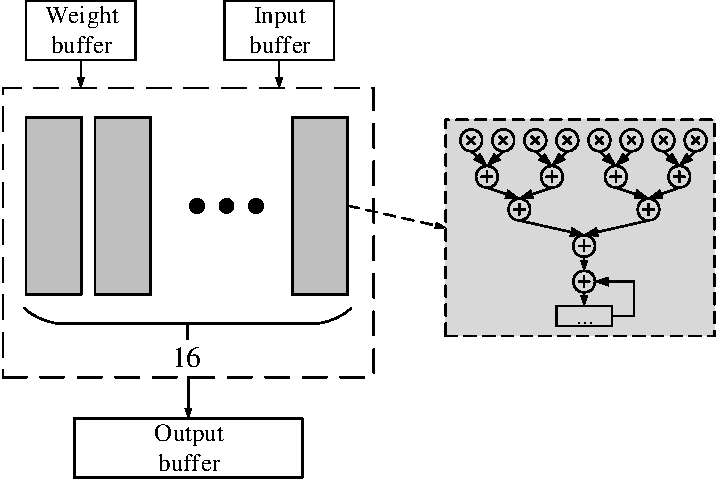
\includegraphics[width=0.75\linewidth]{accelerator}}
    \caption{Baseline CNN accelerator architecture.}
\label{fig:cnn-arch}
\vspace{-1em}
\end{figure}


In order to evaluate the influence of clock 
frequency, we further set the clock to 50 MHz, 100 MHz, and 150 MHz respectively.
A set of neural networks including LeNet, AlexNet, VGG-16 and VGG-19 are used as the benchmark.
Normalized performance the neural network benchmark executed on the accelerators are 
shown in Fig \ref{fig:computing-bound}. It can be found that the 
overall performance of the neural network benchmark
almost increases proportional to the clock frequency. For the larger neural networks, 
the processing remains the computing bound and high frequency design is highly demanded.

\begin{figure}
	\center{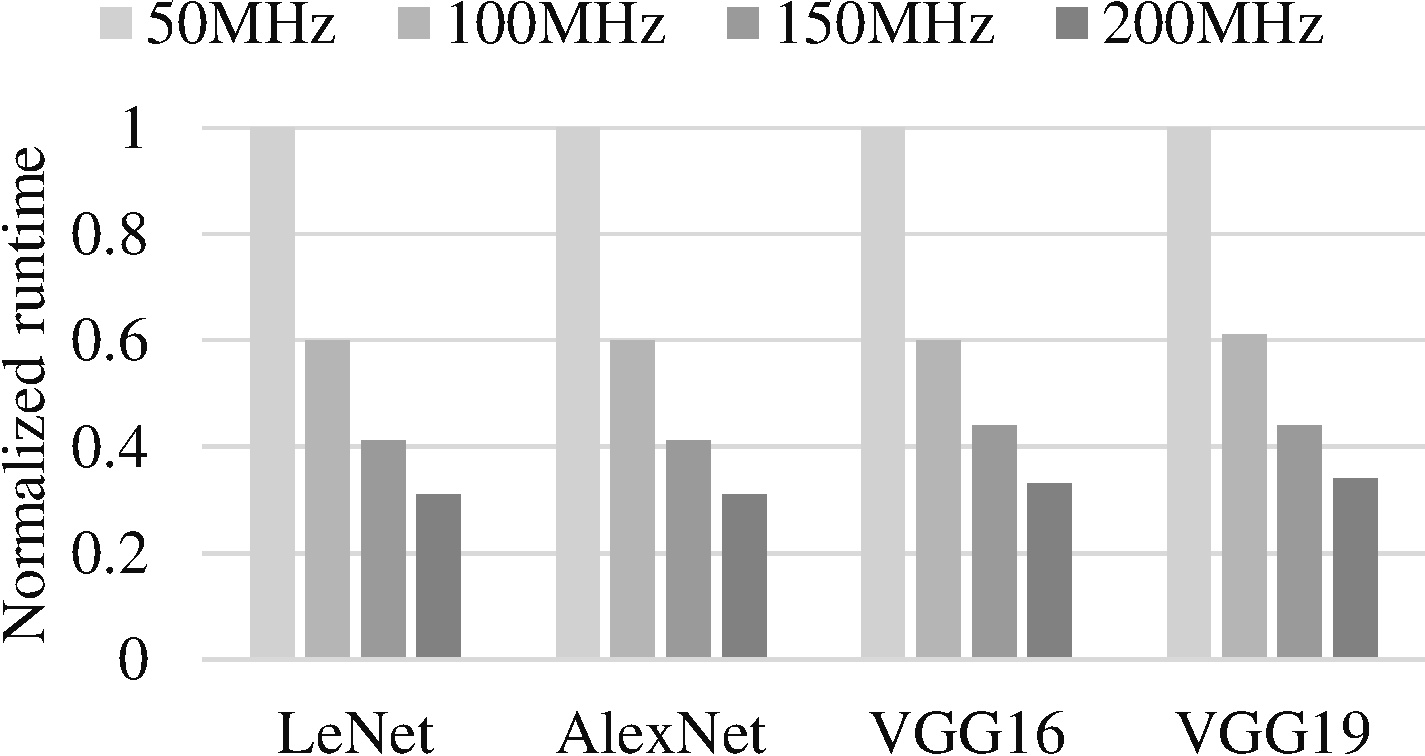
\includegraphics[width=0.75\linewidth]{relative_time}}
    \caption{Normalized performance of neural networks executed on CNN accelerators with different clock frequency.}
\label{fig:computing-bound}
\vspace{-1em}
\end{figure}

In addition, we also obtain the power consumption from SDAccel report. 
The power estimation setup assumes xxxx. Given the power consumption and the performance, 
we calcualted the energy delay product which can be used as an energy efficiency metric.
The energy efficiency is presented in Fig \ref{fig:edp}.
\begin{figure}
	\center{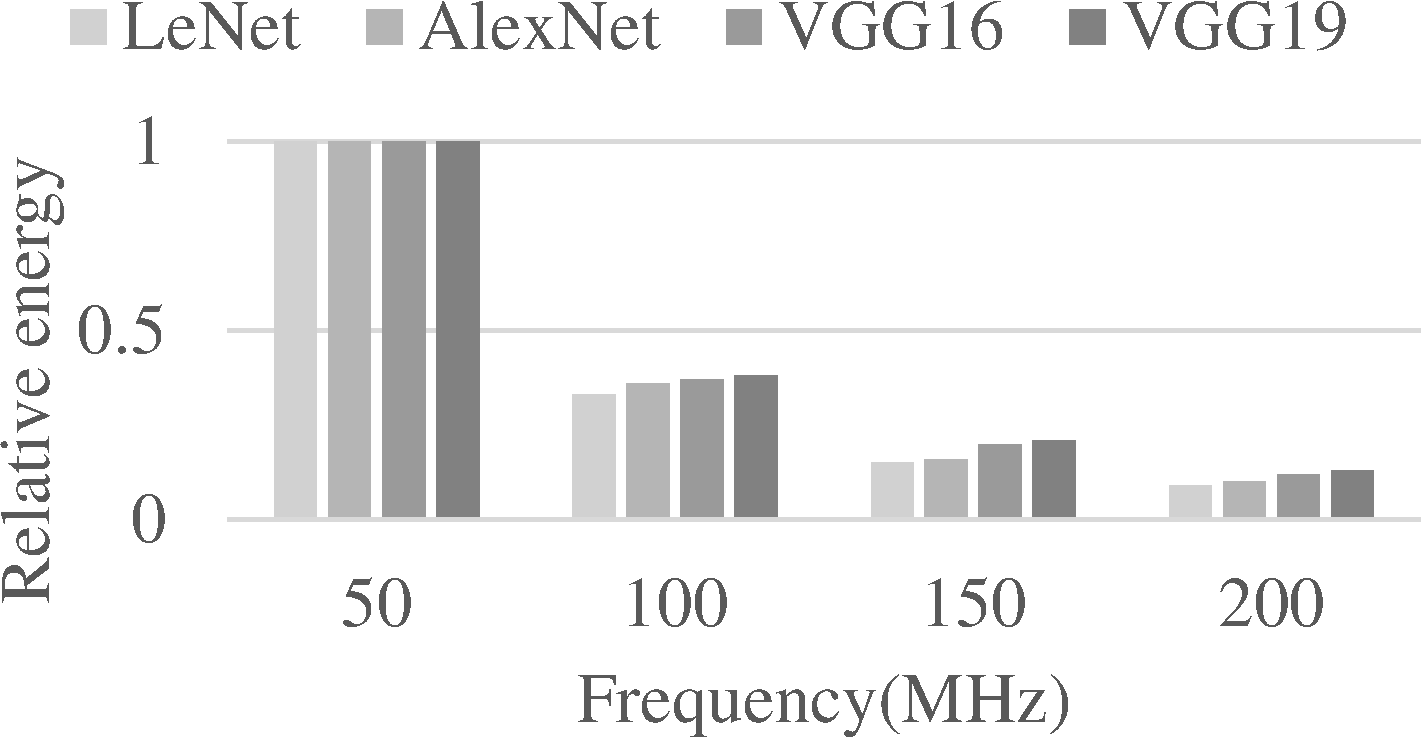
\includegraphics[width=0.75\linewidth]{relative_energy}}
    \caption{Normalized energy-delay product of neural networks executed on CNN accelerators with different clock frequency.}
\label{fig:edp}
\vspace{-1em}
\end{figure}

According to the above experiments, it can be conclcuded that higher clock frequency 
can be beneficial to both the neural network performance and energy efficiency. The 
potential performance and energy efficiency improvement indicates that it is 
worthwhile to boosting the clock of FPGA based CNN accelerators with some minor 
overhead. Detailed overclocking on CNN accelerators will be investigated in 
detail in the rest part of this paper. 

Developing applications that run on FPGAs is without doubt a very different experience from writing programs in software.
Not only is the hardware design process fundamentally different from that of software development, software programmers also often find themselves constantly battling with the much lower \emph{design productivity} in developing hardware designs.

To begin, first time FPGA designers are often put off by the steep learning curve of the complex labyrinth of tools involved.
Beyond that, instead of spending merely seconds to compile and debug a quick-and-dirty proof-of-concept design, software programmers soon also discover that implementing even the simplest FPGA design can consume at least tens of minutes of their development time.
As the size of their designs increase, the run time of these implementation tools quickly increase to hours or even days, greatly limiting the number of possible debug-edit-implement cycles per day.
Indeed, to debug, they may turn to the use of a cycle-accurate simulator. 
Unfortunately, tracing the behaviors of even just a handful of signals through tens of thousands of cycles soon becomes a slow and intractable process.

In this chapter, we explore how the concept of FPGA overlay may be able to alleviate some of these burdens.
We will look at how by using an overlay architecture, designers are able to compile applications to FPGA hardware in merely seconds instead of hours.
We will also look at how overlays are able to help with design portability, as well as to improve debugging capabilities of low-level designs.
Finally, we will explore the challenges and opportunities for future research in this area.


\section{Overview}
%The concept of overlaying a virtual architecture over a physical system is not entirely new -- in networking, for example, virtual overlay networks are routinely constructed on top of the physical infrastructure in modern systems.
On the other hand, the concept of overlaying a virtual architecture over a physical FPGA is only recently gaining traction among researchers, but is already generating a lot of excitements because of their potentials.


% \begin{center}
% \fbox{\begin{minipage}{\linewidth}
% A virtual reconfigurable architecture that overlays on top of the physical FPGA configurable fabric.
% \end{minipage}}
% \end{center}

So what is an FPGA overlay exactly?
Interestingly, because of the unique nature of FPGAs as a flexible configurable hardware, drawing up a precise definition for an FPGA overlay may not be as straightforward as it may seem. 
In this chapter, we will use the following definition as a starting point.

\begin{quote}
An FPGA overlay is a virtual reconfigurable architecture that overlays on top of the physical FPGA configurable fabric.
\end{quote}

From this definition, we can see that an FPGA overlay is a machine architecture that is able to carry out certain computation.  Furthermore, this architecture is \emph{virtual} because the overlay may not necessarily be implemented physically in the final design.  Finally, it is \emph{reconfigurable} because the overlay must be able to support customization or be reprogrammed to support more than one applications.

In other words, an FPGA overlay is a virtual layer of architecture that conceptually locates between the user application and the underlying physical FPGA similar to that shown in \figref{fig:overlay_overview}.
With this additional layer, user applications will no longer be implemented onto the physical FPGA directly.
Instead, the application will be targeted toward the overlay architecture regardless of what the physical FPGA may be.
A separate step will subsequently translate this overlay architecture, together with the application that runs on it, on to the physical FPGA.

\begin{figure}
\centering
\includegraphics[width=0.5\linewidth]{overlay_overview}
\caption{Using an overlay to form a 2-layer approach to FPGA application development.  Overlay may be designed as a virtual FPGA, or it may implement an entirely different compute architecture such as a coarse-grained reconfigurable array (CGRA), vector processor, multi-core process, or even an GPU.}
\label{fig:overlay_overview}
\end{figure}

The easiest way to understand how an FPGA overlay operates in practice, is to consider building a \emph{virtual} FPGA (\textsc{va}) using the configurable fabric of a physical FPGA (\textsc{pa}).  By doing so, you now have an FPGA overlay architecture in the form of \textsc{va} overlaying on top of \textsc{pa}.  We say that \textsc{va} is essentially ``virtual'' because architectural features of \textsc{va} such as its muxes or I/O blocks may not necessarily be present in \textsc{pa}.  Yet, if the overlay is constructed correctly, any design that was originally targeting \textsc{va} may now execute unmodified on \textsc{pa} without knowing its details.

However, the power of employing FPGA overlay is not limited to making virtual FPGAs only.
On the contrary, taking advantage of FPGA's general-purpose configurable fabric, many researchers have demonstrated the benefits of overlays that implement entirely different computing architectures such as 
multi-core processor system, coarse-grained reconfigurable arrays (CGRAs), or even general-purpose graphic processing units (GPUs).

Now, using a multi-core processor overlay as an example, it should be apparent how overlays are able to improve a software programmer's design productivity.
Instead of working with unfamiliar hardware-centric tools and design methodologies, software programmers are now possible to utilize FPGAs as accelerators simply by writing programs that target a familiar architecture.
In general, one benefit of using FPGA overlay is that it is able to bridge between the often software-inclined user and the low-level FPGA hardware fabric.

Of course, if an application can be readily accelerated on a multi-core processor overlay implemented using FPGAs, then it is understandably begging the question: why not simply run the design on an actual high-performance multi-core processor instead?
The answer to this question, indeed, is the key challenge that will guide the future research on overlay designs --- While an overlay offers many desirable features to software programmable such as improved design productivity, the additional layer on top of the physical FPGA inevitably introduces additional performance penalty to the system.
A good overlay design must therefore ensure that despite the performance penalty introduced, the overall acceleration offered by FPGA must remain competitive for the accelerator system to be worthwhile.
Furthermore, it must provided added value beyond a solution with a fixed general-purpose architecture.
One such added value is the ability to customize the overlay for the particular application or group of applications concerned for sake of performance or power-efficiency.



\iffalse

Unfortunately, and also fortunately, because of the flexibility of FPGAs, the exact definition of an overlay can sometimes be difficult to precisely define.  If you implement a Commodore 64 system on an FPGA so you can play your favorite 8-bit games on FPGA, are you implementing a game system or is it already a ``overlay'' in the form of a CPU system?
What if you now upgrade this classic system to become a massively multi-core processor system for parallel execution of game code?  Would that make it more of an overlay than the simple soft CPU core?


In the straightest sense according to the above definition, a simple soft CPU core implemented on an FPGA can be regarded as an overlay -- it is virtual as you can implement the same CPU differently on different FPGAs, providing portability and compatibility.  At the same time, it is also reconfigurable, as you can obviously execute a broad range of applications on this CPU by programming it with different software.


In practice, however, the concept of an FPGA overlay is a lot far reaching than a simple soft CPU core.  It encompasses all sorts of compute architectures one can imagine, with many of them designed specifically for the purpose of serving as an overlay.  These overlays are specifically designed for the goal at hand: for virtualization, for efficiency, for power-performance tradeoff, for design productivity, etc.  They are also specially designed for use in FPGA with low overhead.

\fi

%Sometimes such overlay may not even literally exist in the final physical design.  For example a word-based FPGA may exist only in the form of design constraint or is embedded in the design language, while its architectural features may not necessarily be implemented on the FPGA (e.g. any unused word-mux defined in the architecture doesn't need to be implemented.)  It is as opposed to constructing this word-based FPGA physically on silicon.

\subsection{Coarse-Grained Architectures}
In most cases, FPGA overlays are essentially coarse-grained architectures that are built on top of the physical fine-grained configurable fabric.
As their names suggest, the basic idea of a coarse-grained architecture is to reduce the configuration granularity of an FPGA from its physical fine-grained configurable fabric such as LUTs to one with coarser reconfiguration granularity.
In some cases, such coarse-grained blocks may refer simply to arithmetic blocks of moderate sizes such as adders, multipliers, or digital signal processing blocks of some sort.
In other cases, such coarse-grained blocks may refer to very complex microprocessors connected with sophisticated network-on-chip.
Regardless of the implementation, the central goal of any coarse-grained architecture remains the same: to improve power-performance of the system by trading off design flexibility.

%From the perspective of overlay design, coarse-grained architectures are very attractive.
%Not only do they have clearly demonstrated power-performance advantages, they are also good candidates to serve as a design productivity improvement choice.

In addition, because of their reduced configuration flexibility, coarse-grained architectures can also enable design methodologies that are more productive than traditional hardware design flow.
In particular, coarse-grained architectures improve a designer's productivity in two important ways.
First, by constraining the flexibility of an FPGA, a coarse-grained architecture reduces the design space significantly, which has a net effect of reducing implementation tool flow run time considerably \cite{lavin2011}. 
In addition, many coarse-grained architectures implement compute models that are more familiar to software designers, considerably lowering the barrier-to-entry to employ such designs.  For instance, many recent overlays are implemented as coarse-grained reconfigurable arrays (CGRAs), where computation is carried out by a connected array of processing elements (PEs).
Instead of implementing the user application using low-level configurable logic of the FPGA, these operations are translated into computational tasks that take place in the PEs.
To many software programmers, programming a parallel processor array, while a daunting task in its own right, is arguably a lot more approachable than to implement designs on the native FPGA configurable fabric.
As such, it is not surprising that many recent overlay designs are built on top of an underlying coarse-grained reconfigurable array \cite{kissler2006dynamically,ferreira2011fpga,shukla2006quku,Lin:2012:EDC:2460216.2460227,capalijia2013pipelined,dspoverlay}.





\section{Benefits of Overlays}
As a virtualization layer that sits between a user application and the physical configurable fabric, an FPGA overlay inherits many of the benefits that software programmers have learned to expect from their CPU virtualization experience --- portability, compatibility, manageability, isolation, etc.  On top of that, employing FPGA overlays has also been demonstrated as a good way to improve a designer's productivity through improved compilation speed and better debugging support.  Along the same line, by carefully partitioning the complex hardware-software design flow around an intermediate overlay layer, it is also possible to provide separation of concerns between software and hardware engineers in the design team.
The overlay essentially acts as a bridge between the two teams, while allowing the overall system to take advantage of the FPGA resources efficiently.

\subsection{Virtualization}
Virtualization of FPGA resources has long been an active area of research since the early days of reconfigurable computing.  These pioneering works have demonstrated many of the possibilities as well as challenges associated with virtualizing hardware resources that are not designed to be time-multiplexed.  A common trend among these early works was that virtualization can be used as a mean to provide the designers and/or tools the illusion of having infinite hardware resources.  Early works by Trimberger et al~\cite{Trimberger97}, virtual wire\cite{virtualwire} and SCORE \cite{score}, for instances, gave the users the illusion of a system with unlimited FPGA resources through carefully structured hardware/CAD system.  Others have studied the problem of time-sharing of FPGA resources from an operating system's perspective as a way to provide shared accelerator resources among users/processes. \cite{Lubbers:2009:RMP:1596532.1596540,SoTECS08,Fu:2005:FCCM}.

As the concept of FPGA overlay continues to mature, the idea of virtualizing FPGAs has taken on a new focus.  As an overlay, virtualizing FPGAs allows an additional benefit of providing a compatibility and portability layer for FPGA designs.  In the work of Zuma~\cite{zuma2012}, for instance, virtual, embedded FPGAs were proposed.  By providing a virtual FPGA layer, the authors demonstrated that it is possible to execute the same netlist on multiple FPGAs from competing vendors using multiple different design tools.

\iffalse
\subsection{Improved Design Productivity}
An important benefit of using FPGA overlays is that they promise to improve designer's productivity in developing FPGA applications.
Design productivity is hard to measure, but has long been regarded as one of the key barrier-to-entry for novice users to start using FPGAs for their applications \cite{SoFpl06}.
In particular, FPGA overlays are particularly helpful in addressing two important aspects of this design productivity challenges: 
\begin{itemize}
\item Reduced compilation time
\item Application debug
\end{itemize}
\fi

\subsection{Reduced Compilation Time}
A key difference in design experience between software compilation and implementing FPGA designs rests on their drastically different run time of the involved tools.
With modern compiler technologies, software compilation has already become a straightforward, predictable, and most importantly, very rapid process.
Compiling even a relatively complex piece of software application rarely take longer than a few minutes on a reasonably fast computer.
On the other hand, implementing applications for FPGAs involves a complex labyrinth of low-level tools that are convoluted, unpredictable, and takes a long time to complete.
Compiling even the smallest design may take tens of minutes, while spending hours or even days on some of the largest designs are not unheard of.
Unfortunately, this 2 orders of magnitude difference in run time, together with the unpredictable nature\footnote{Placing and routing a design on nearly full FPGA, for example, may or may not succeed depending on the random algorithms involved.} and the often-mystical error reporting mechanisms\footnote{To see this, try to explain to a first-time software programmer why a functionally correct design in simulation may end up with an error message about timing violation on a net with an unknown name in the report.  Then, also try to explain to the programmer how to resolve that timing error.}, are all contributing to a very high barrier-to-entry that shies away most first time software programmers.
Technically, this much longer run time of the tools also significantly reduces the number of possible debug-edit-implement cycles per day, causing project delays as well as lowered productivity of the designers.

By using an overlay as intermediate compilation target, together with careful crafting of the design process, researchers have demonstrated how such lengthy hardware development process can be reduced significantly.
For example, in the work of Intermediate Fabric\cite{Coole2010Intermediate}, an intermediate coarse-grained reconfigurable fabric was introduced as an overlay.
With the overlay architecture, the average place and route times for the tested benchmark were significantly reduced by more than 500 times.

Similarly in the work of QuickDough, a coarse-grained reconfigurable array was used as overlay to accelerate compute intensive loop kernels.  Loops are scheduled to execute on the CGRA instead of compiling to the reconfigurable fabric.  As a result, when compared to manually generating custom hardware for the loops using standard hardware tools, up to 3 orders of magnitude reduction in compilation time was demonstrated.

\subsection{Improved Debugging Capabilities}
Unlike many software development frameworks where a range of debugging facilities and methodologies are readily available, tools for debugging applications that target FPGA-based systems are still in their infancy.
Traditional FPGA design methodologies rely heavily on cycle-accurate simulations for application development and debugging.
While such simulations are invaluable to understand the low-level operation of the FPGA, they are slow, tedious and provide only limited information about the run-time behavior of the design.
To monitor run-time behavior of a design, users must rely on even more complex in-system emulation facilities or even external testing hardware.
Taking advantage of FPGA overlays, researchers have demonstrated some promising results addressing the need for better debugging tools.

For instance, in a series of work by Hung and Wilton \cite{Hung:2014:VLSI,Hung:2013:TSO:2435264.2435272}, an overlay network was incorporated into FPGA design to facilitate insertion of trace buffers after a design has been placed and routed.
By carefully controlling the signal routes to utilize only unoccupied resources in the FPGA, they have demonstrated efficient ways to dynamically select and monitor signals during run time.

In other cases, since the overlay layer enables a virtual computing paradigm for the application developer that is different from the underlying FPGA, they also enable new debugging strategies that are more suitable to the designer. For instance in MARC, debugging the user-specified OpenCL applications that run on the generated multi-core architecture can follow traditional software debugging methodologies instead of relying on low level FPGA tools.
Not only can it greatly increase the abstraction level, but it can also allow a debugging strategy that matches the user's expectation.

\subsection{Separation of Hardware and Software Concerns}
With careful planning, it is also possible to take advantage of the 2-layer design approach offered by FPGA overlays as a natural division point between hardware and software development efforts.
Recall from \figref{fig:overlay_overview} that implementing designs via an FPGA overlay involves 2 steps: user applications must first be mapped to the overlay architecture, which is subsequently implemented to the physical fabric in a second step.
In many cases, the overlay architectures are designed so they can efficiently support the computational model expected by the model.
As a result, mapping of software applications to the overlay is usually more intuitive to software programmers than to map the same application to the physical FPGA fabric in one step.
On the other hand, mapping the overlay and the user application to the physical fabric involves intimate knowledge about the FPGA hardware implementation process.
This task is best left to a separate hardware team.
Consequently, one benefit of having an overlay is that the hardware team may now devote their efforts exclusively on implementing the relatively well-structured overlay on the fabric, rather than to implement many individual applications.
The hardware team can be more focused, and can perceivably create a better, highly optimized hardware design.

For example in the work of MARC\cite{lavin2011}, a multi-core processor-like architecture was used as an intermediate compilation target.
In this project, user applications are expressed as OpenCL programs.
To implement these applications, they are first compiled as an application-specific multi-core processor, which is subsequently implemented on the physical FPGA in a separate process.
With this set up, users no longer need to understand the detailed implementation of their algorithm on FPGAs.
Instead, they write essentially standard OpenCL programs, and focuses exclusively on writing the best code for the accelerated architecture assumed.
The task to map their OpenCL code into custom core on the target overlay, and to implement that overlay on the FPGA fabric, was left to a separate team.

In their case studies, the resulting application achieves about one third of the speedup when compared to fully custom designs.
Yet with the 2-layer approach using OpenCL, the design effort with MARC is significantly lower when compared to making a custom design of the same application.





The concept of overlaying a virtual architecture over a physical system is not entirely new -- in networking, for example, virtual overlay networks are routinely constructed on top of the physical infrastructure in modern systems.
On the other hand, the concept of overlaying a virtual architecture over a physical FPGA is only recently gaining traction among researchers, but is already generating a lot of excitements because of their potentials.


% \begin{center}
% \fbox{\begin{minipage}{\linewidth}
% A virtual reconfigurable architecture that overlays on top of the physical FPGA configurable fabric.
% \end{minipage}}
% \end{center}

So what is an FPGA overlay exactly?
Interestingly, because of the unique nature of FPGAs as a flexible configurable hardware, drawing up a precise definition for an FPGA overlay may not be as straightforward as it may seem. 
In this chapter, we will use the following definition as a starting point.

\begin{quote}
An FPGA overlay is a virtual reconfigurable architecture that overlays on top of the physical FPGA configurable fabric.
\end{quote}

From this definition, we can see that an FPGA overlay is a machine architecture that is able to carry out certain computation.  Furthermore, this architecture is \emph{virtual} because the overlay may not necessarily be implemented physically in the final design.  Finally, it is \emph{reconfigurable} because the overlay must be able to support customization or be reprogrammed to support more than one applications.

In other words, an FPGA overlay is a virtual layer of architecture that conceptually locates between the user application and the underlying physical FPGA similar to that shown in \figref{fig:overlay_overview}.
With this additional layer, user applications will no longer be implemented onto the physical FPGA directly.
Instead, the application will be targeted toward the overlay architecture regardless of what the physical FPGA may be.
A separate step will subsequently translate this overlay architecture, together with the application that runs on it, on to the physical FPGA.

\begin{figure}
\centering
\includegraphics[width=0.5\linewidth]{overlay_overview}
\caption{Using an overlay to form a 2-layer approach to FPGA application development.  Overlay may be designed as a virtual FPGA, or it may implement an entirely different compute architecture such as a coarse-grained reconfigurable array (CGRA), vector processor, multi-core process, or even an GPU.}
\label{fig:overlay_overview}
\end{figure}

The easiest way to understand how an FPGA overlay operates in practice, is to consider building a \emph{virtual} FPGA (\textsc{va}) using the configurable fabric of a physical FPGA (\textsc{pa}).  By doing so, you now have an FPGA overlay architecture in the form of \textsc{va} overlaying on top of \textsc{pa}.  We say that \textsc{va} is essentially ``virtual'' because architectural features of \textsc{va} such as its muxes or I/O blocks may not necessarily be present in \textsc{pa}.  Yet, if the overlay is constructed correctly, any design that was originally targeting \textsc{va} may now execute unmodified on \textsc{pa} without knowing its details.

However, the power of employing FPGA overlay is not limited to making virtual FPGAs only.
On the contrary, taking advantage of FPGA's general-purpose configurable fabric, many researchers have demonstrated the benefits of overlays that implement entirely different computing architectures such as 
multi-core processor system, coarse-grained reconfigurable arrays (CGRAs), or even general-purpose graphic processing units (GPUs).

Now, using a multi-core processor overlay as an example, it should be apparent how overlays are able to improve a software programmer's design productivity.
Instead of working with unfamiliar hardware-centric tools and design methodologies, software programmers are now possible to utilize FPGAs as accelerators simply by writing programs that target a familiar architecture.
In general, one benefit of using FPGA overlay is that it is able to bridge between the often software-inclined user and the low-level FPGA hardware fabric.

Of course, if an application can be readily accelerated on a multi-core processor overlay implemented using FPGAs, then it is understandably begging the question: why not simply run the design on an actual high-performance multi-core processor instead?
The answer to this question, indeed, is the key challenge that will guide the future research on overlay designs --- While an overlay offers many desirable features to software programmable such as improved design productivity, the additional layer on top of the physical FPGA inevitably introduces additional performance penalty to the system.
A good overlay design must therefore ensure that despite the performance penalty introduced, the overall acceleration offered by FPGA must remain competitive for the accelerator system to be worthwhile.
Furthermore, it must provided added value beyond a solution with a fixed general-purpose architecture.
One such added value is the ability to customize the overlay for the particular application or group of applications concerned for sake of performance or power-efficiency.



\iffalse

Unfortunately, and also fortunately, because of the flexibility of FPGAs, the exact definition of an overlay can sometimes be difficult to precisely define.  If you implement a Commodore 64 system on an FPGA so you can play your favorite 8-bit games on FPGA, are you implementing a game system or is it already a ``overlay'' in the form of a CPU system?
What if you now upgrade this classic system to become a massively multi-core processor system for parallel execution of game code?  Would that make it more of an overlay than the simple soft CPU core?


In the straightest sense according to the above definition, a simple soft CPU core implemented on an FPGA can be regarded as an overlay -- it is virtual as you can implement the same CPU differently on different FPGAs, providing portability and compatibility.  At the same time, it is also reconfigurable, as you can obviously execute a broad range of applications on this CPU by programming it with different software.


In practice, however, the concept of an FPGA overlay is a lot far reaching than a simple soft CPU core.  It encompasses all sorts of compute architectures one can imagine, with many of them designed specifically for the purpose of serving as an overlay.  These overlays are specifically designed for the goal at hand: for virtualization, for efficiency, for power-performance tradeoff, for design productivity, etc.  They are also specially designed for use in FPGA with low overhead.

\fi

%Sometimes such overlay may not even literally exist in the final physical design.  For example a word-based FPGA may exist only in the form of design constraint or is embedded in the design language, while its architectural features may not necessarily be implemented on the FPGA (e.g. any unused word-mux defined in the architecture doesn't need to be implemented.)  It is as opposed to constructing this word-based FPGA physically on silicon.

\subsection{Coarse-Grained Architectures}
In most cases, FPGA overlays are essentially coarse-grained architectures that are built on top of the physical fine-grained configurable fabric.
As their names suggest, the basic idea of a coarse-grained architecture is to reduce the configuration granularity of an FPGA from its physical fine-grained configurable fabric such as LUTs to one with coarser reconfiguration granularity.
In some cases, such coarse-grained blocks may refer simply to arithmetic blocks of moderate sizes such as adders, multipliers, or digital signal processing blocks of some sort.
In other cases, such coarse-grained blocks may refer to very complex microprocessors connected with sophisticated network-on-chip.
Regardless of the implementation, the central goal of any coarse-grained architecture remains the same: to improve power-performance of the system by trading off design flexibility.

%From the perspective of overlay design, coarse-grained architectures are very attractive.
%Not only do they have clearly demonstrated power-performance advantages, they are also good candidates to serve as a design productivity improvement choice.

In addition, because of their reduced configuration flexibility, coarse-grained architectures can also enable design methodologies that are more productive than traditional hardware design flow.
In particular, coarse-grained architectures improve a designer's productivity in two important ways.
First, by constraining the flexibility of an FPGA, a coarse-grained architecture reduces the design space significantly, which has a net effect of reducing implementation tool flow run time considerably \cite{lavin2011}. 
In addition, many coarse-grained architectures implement compute models that are more familiar to software designers, considerably lowering the barrier-to-entry to employ such designs.  For instance, many recent overlays are implemented as coarse-grained reconfigurable arrays (CGRAs), where computation is carried out by a connected array of processing elements (PEs).
Instead of implementing the user application using low-level configurable logic of the FPGA, these operations are translated into computational tasks that take place in the PEs.
To many software programmers, programming a parallel processor array, while a daunting task in its own right, is arguably a lot more approachable than to implement designs on the native FPGA configurable fabric.
As such, it is not surprising that many recent overlay designs are built on top of an underlying coarse-grained reconfigurable array \cite{kissler2006dynamically,ferreira2011fpga,shukla2006quku,Lin:2012:EDC:2460216.2460227,capalijia2013pipelined,dspoverlay}.





\section{Benefits of Overlays}
As a virtualization layer that sits between a user application and the physical configurable fabric, an FPGA overlay inherits many of the benefits that software programmers have learned to expect from their CPU virtualization experience --- portability, compatibility, manageability, isolation, etc.  On top of that, employing FPGA overlays has also been demonstrated as a good way to improve a designer's productivity through improved compilation speed and better debugging support.  Along the same line, by carefully partitioning the complex hardware-software design flow around an intermediate overlay layer, it is also possible to provide separation of concerns between software and hardware engineers in the design team.
The overlay essentially acts as a bridge between the two teams, while allowing the overall system to take advantage of the FPGA resources efficiently.

\subsection{Virtualization}
Virtualization of FPGA resources has long been an active area of research since the early days of reconfigurable computing.  These pioneering works have demonstrated many of the possibilities as well as challenges associated with virtualizing hardware resources that are not designed to be time-multiplexed.  A common trend among these early works was that virtualization can be used as a mean to provide the designers and/or tools the illusion of having infinite hardware resources.  Early works by Trimberger et al~\cite{Trimberger97}, virtual wire\cite{virtualwire} and SCORE \cite{score}, for instances, gave the users the illusion of a system with unlimited FPGA resources through carefully structured hardware/CAD system.  Others have studied the problem of time-sharing of FPGA resources from an operating system's perspective as a way to provide shared accelerator resources among users/processes. \cite{Lubbers:2009:RMP:1596532.1596540,SoTECS08,Fu:2005:FCCM}.

As the concept of FPGA overlay continues to mature, the idea of virtualizing FPGAs has taken on a new focus.  As an overlay, virtualizing FPGAs allows an additional benefit of providing a compatibility and portability layer for FPGA designs.  In the work of Zuma~\cite{zuma2012}, for instance, virtual, embedded FPGAs were proposed.  By providing a virtual FPGA layer, the authors demonstrated that it is possible to execute the same netlist on multiple FPGAs from competing vendors using multiple different design tools.

\iffalse
\subsection{Improved Design Productivity}
An important benefit of using FPGA overlays is that they promise to improve designer's productivity in developing FPGA applications.
Design productivity is hard to measure, but has long been regarded as one of the key barrier-to-entry for novice users to start using FPGAs for their applications \cite{SoFpl06}.
In particular, FPGA overlays are particularly helpful in addressing two important aspects of this design productivity challenges: 
\begin{itemize}[nosep]
\item Reduced compilation time
\item Application debug
\end{itemize}
\fi

\subsection{Reduced Compilation Time}
A key difference in design experience between software compilation and implementing FPGA designs rests on their drastically different run time of the involved tools.
With modern compiler technologies, software compilation has already become a straightforward, predictable, and most importantly, very rapid process.
Compiling even a relatively complex piece of software application rarely take longer than a few minutes on a reasonably fast computer.
On the other hand, implementing applications for FPGAs involves a complex labyrinth of low-level tools that are convoluted, unpredictable, and takes a long time to complete.
Compiling even the smallest design may take tens of minutes, while spending hours or even days on some of the largest designs are not unheard of.
Unfortunately, this 2 orders of magnitude difference in run time, together with the unpredictable nature\footnote{Placing and routing a design on nearly full FPGA, for example, may or may not succeed depending on the random algorithms involved.} and the often-mystical error reporting mechanisms\footnote{To see this, try to explain to a first-time software programmer why a functionally correct design in simulation may end up with an error message about timing violation on a net with an unknown name in the report.  Then, also try to explain to the programmer how to resolve that timing error.}, are all contributing to a very high barrier-to-entry that shies away most first time software programmers.
Technically, this much longer run time of the tools also significantly reduces the number of possible debug-edit-implement cycles per day, causing project delays as well as lowered productivity of the designers.

By using an overlay as intermediate compilation target, together with careful crafting of the design process, researchers have demonstrated how such lengthy hardware development process can be reduced significantly.
For example, in the work of Intermediate Fabric\cite{Coole2010Intermediate}, an intermediate coarse-grained reconfigurable fabric was introduced as an overlay.
With the overlay architecture, the average place and route times for the tested benchmark were significantly reduced by more than 500 times.

Similarly in the work of QuickDough, a coarse-grained reconfigurable array was used as overlay to accelerate compute intensive loop kernels.  Loops are scheduled to execute on the CGRA instead of compiling to the reconfigurable fabric.  As a result, when compared to manually generating custom hardware for the loops using standard hardware tools, up to 3 orders of magnitude reduction in compilation time was demonstrated.

\subsection{Improved Debugging Capabilities}
Unlike many software development frameworks where a range of debugging facilities and methodologies are readily available, tools for debugging applications that target FPGA-based systems are still in their infancy.
Traditional FPGA design methodologies rely heavily on cycle-accurate simulations for application development and debugging.
While such simulations are invaluable to understand the low-level operation of the FPGA, they are slow, tedious and provide only limited information about the run-time behavior of the design.
To monitor run-time behavior of a design, users must rely on even more complex in-system emulation facilities or even external testing hardware.
Taking advantage of FPGA overlays, researchers have demonstrated some promising results addressing the need for better debugging tools.

For instance, in a series of work by Hung and Wilton \cite{Hung:2014:VLSI,Hung:2013:TSO:2435264.2435272}, an overlay network was incorporated into FPGA design to facilitate insertion of trace buffers after a design has been placed and routed.
By carefully controlling the signal routes to utilize only unoccupied resources in the FPGA, they have demonstrated efficient ways to dynamically select and monitor signals during run time.

In other cases, since the overlay layer enables a virtual computing paradigm for the application developer that is different from the underlying FPGA, they also enable new debugging strategies that are more suitable to the designer. For instance in MARC, debugging the user-specified OpenCL applications that run on the generated multi-core architecture can follow traditional software debugging methodologies instead of relying on low level FPGA tools.
Not only can it greatly increase the abstraction level, but it can also allow a debugging strategy that matches the user's expectation.

\subsection{Separation of Hardware and Software Concerns}
With careful planning, it is also possible to take advantage of the 2-layer design approach offered by FPGA overlays as a natural division point between hardware and software development efforts.
Recall from \figref{fig:overlay_overview} that implementing designs via an FPGA overlay involves 2 steps: user applications must first be mapped to the overlay architecture, which is subsequently implemented to the physical fabric in a second step.
In many cases, the overlay architectures are designed so they can efficiently support the computational model expected by the model.
As a result, mapping of software applications to the overlay is usually more intuitive to software programmers than to map the same application to the physical FPGA fabric in one step.
On the other hand, mapping the overlay and the user application to the physical fabric involves intimate knowledge about the FPGA hardware implementation process.
This task is best left to a separate hardware team.
Consequently, one benefit of having an overlay is that the hardware team may now devote their efforts exclusively on implementing the relatively well-structured overlay on the fabric, rather than to implement many individual applications.
The hardware team can be more focused, and can perceivably create a better, highly optimized hardware design.

For example in the work of MARC\cite{lavin2011}, a multi-core processor-like architecture was used as an intermediate compilation target.
In this project, user applications are expressed as OpenCL programs.
To implement these applications, they are first compiled as an application-specific multi-core processor, which is subsequently implemented on the physical FPGA in a separate process.
With this set up, users no longer need to understand the detailed implementation of their algorithm on FPGAs.
Instead, they write essentially standard OpenCL programs, and focuses exclusively on writing the best code for the accelerated architecture assumed.
The task to map their OpenCL code into custom core on the target overlay, and to implement that overlay on the FPGA fabric, was left to a separate team.

In their case studies, the resulting application achieves about one third of the speedup when compared to fully custom designs.
Yet with the 2-layer approach using OpenCL, the design effort with MARC is significantly lower when compared to making a custom design of the same application.





\section{Types of Overlays}
%Over the years, quite a few works on FPGA overlays have been developed.
In this section, we will take a quick walk through some of them and also look at various types of FPGA overlays that have been explored in the past decade.

\subsection{Virtual FPGAs}
To begin, one of the most easiest to understand categories of overlay are virtual FPGAs\cite{vFPGA,zuma2012,Grant2011Malibu,Coole2010Intermediate,Koch2013CI}. They are built either virtually or physically on top of off-the-shelf FPGA devices. These overlays have different configuration granularity but typically feature coarser configuration granularity than a typical FPGA device. Similar to virtual machines running on a typical computer, such virtual FPGA provides an additional layer that improves application portability and compatibility. Furthermore, because of the coarser-grained configurable fabric, implementing designs on such overlay is relatively easier than on a fine-grained device. However, the additional layer imposes restrictions on the underlying fabrics' capability and usually results in moderate hardware overhead and timing degradation.

In one of the earlier works, Lysecky et al. developed a relatively fine-grained virtual FPGA as firm cores expressed as structural VHDL \cite{vFPGA}. The virtual layer provides effective portability yet incurs relatively high performance and hardware overhead.
In \cite{Grant2011Malibu}, Grant et al. proposed a time-multiplexed virtual FPGA CAD framework MALIBU. The virtual FPGA used in MALIBU has both fine-grain and coarse-grain processing elements integrated into each logic cluster and can be used to reduce the compilation time significantly with moderate timing penalty. Around the same time, Coole and Stitt also proposed another island-style coarse-grained overlay called Intermediate Fabric \cite{Coole2010Intermediate}. It uses coarse-grained operators such as adders instead of logic clusters and routes data through 8 to 32 bit buses achieving both portability and fast compilation. Finally, Koch et al. developed a fine-grained FPGA overlay in \cite{Koch2013CI} to implement customized instructions on FPGAs from different vendors providing a portable application consisting of a program binary and an overlay configuration in a completely heterogeneous environment.

\subsection{Coarse-Grained Reconfigurable Arrays}
Another category of overlay architecture commonly employed is in the form of coarse-grained reconfigurable arrays (CGRAs) \cite{kissler2006dynamically, ferreira2011fpga, shukla2006quku, Lin:2012:EDC:2460216.2460227,capalijia2013pipelined, dspoverlay}. The use of CGRAs provides an efficient tradeoff between flexibility of software and performance of hardware especially for compute intensive applications as demonstrated by numerous earlier works \cite{tessier01reconfigurable,compton02reconfigurable}.
%Indeed, CGRAs on FPGA and ASIC have many similarities in terms of the scheduling algorithm and array structure. However, they have quite different trade-offs between flexibility and performance. In a nutshell, CGRAs on ASIC emphasize more on flexibility to cover more applications or at least a domain of applications, while FPGAs' inherent programmability greatly alleviates the concern. Instead, CGRAs on FPGA may take advantage of the configurability of the underlying fabric to allow more intensive customization tailored to the target application for better performance and lower hardware overhead.

In one of the earlier works in the area, Kissler et al. developed WPPA (weakly programmable processor array), a VLIW architecture based parameterizable CGRA overlay~\cite{kissler2006dynamically}. It featured an interconnection wrapper unit for each processing element (PE) that could be used for dynamic CGRAs topology customization. 
%Unfortunately, programming and compilation on WPPA were not presented. 
Around the same time in \cite{shukla2006quku}, a customized CGRA overlay called QUKU was developed for DSP algorithms. It had a two-level configuration capability, while the high-speed configuration was used for operator reuse within an application and low-speed reconfiguration was used for optimization between different applications. 
%Nevertheless, the hardware infrastructure was consist of simple operation elements which can only be adapted to a few specified DSP algorithms.
In \cite{ferreira2011fpga}, Ferreira et al. proposed a heterogeneous CGRA overlay with a global multi-stage interconnection on FPGA. Compiling applications onto the overlay took only milliseconds for smaller DFGs. 
%However, the global multi-stage interconnection required multiple stages for communication between each pair of PEs and resulted in either low implementation frequency or large communication latency in terms of cycles. In addition, there was no intermediate storage except the pipeline registers in the CGRA and it limited the performance of the operation scheduling.
In \cite{Lin:2012:EDC:2460216.2460227}, Lin and So also proposed a soft CGRA overlay for rapid compilation.  In addition, they demonstrated that by customizing the overlay connection between PEs on a per-application basis, improvement in energy-efficiency could be obtained in the expense of longer tool run time.
The authors in \cite{capalijia2013pipelined} built a generic high speed mesh CGRA overlay using the elastic pipeline technique to achieve the maximum throughput. It adopted a data-driven execution flow and was suitable for smaller pipelined DFG execution.
%, while it would be difficult to handle applications with random IO access.
Recently in \cite{dspoverlay}, Jain et al. also proposed an overlay that is constructed around the primitive FPGA DSP blocks to achieve high-frequency implementation and high throughput result.
Also, in \cite{adjustable2015}, Coole and Stitt proposed to provide the overlay with limited flexibility instead of full configurability specifically to a group of design. With this customization, the area overhead was reduced significantly.




%In general, previous CGRA overlays have demonstrated the promising performance acceleration capability for compute intensive applications. They typically take DFG as design entry and focus on hardware infrastructure design as well as corresponding mapping and scheduling. However, they are still lack of consideration on proper loop unrolling for DFG generation, on-chip buffering, the communication with host and even end-to-end performance which are essential for FPGA accelerator design especially from a HW/SW co-design engineer's perspective.

\subsection{Processor-Like Overlays}
A third category of overlay moves away from the traditional FPGA architectures and instead explores using processor-like designs as an intermediate layer.
The main concern for works in this category are usually compatibility and usability of the overlay from a user's perspective.  To provide the necessary performance, these overlay architectures usually feature a high degree of control and provide ample of data parallelism to make them suitable for FPGA accelerations.
As an early attempt, Yiannacouras et al. explored the use of a fine-grained scalable vector processor for code acceleration in embedded systems \cite{Yiannacouras2009FPS}.
Later in \cite{Guy2012VENICE}, Severance and Lemieux proposed a soft vector processor named VENICE to allow easy FPGA application development.  It accepts simple C program as input and execute the code on the highly optimized vector processor on the FPGA for performance.
%
%Various processor architectures have been implemented as overlays on top of FPGAs and have been demonstrated to be efficient solutions in many occasions. Soft general purpose processors and soft vector processors are presented in \cite{microblaze, nios} and \cite{Yiannacouras2009FPS, Guy2012VENICE} respectively. 
%
In the work of MARC, Lebedev et al. explored the use of a many-core processor template as an intermediate compilation target \cite{Lebedev2010}.  In that work, they have demonstrated improved usability with the model while also highlighting the need for customizing computational cores for sake of performance.
To explore the integration between processor and FPGA accelerators, a portable machine model with multiple computing architectures called MURAC was explored in \cite{Hamilton:14:FPL}.
Finally, a GPU-like overlay was proposed in \cite{Jeffrey2011potential} that demonstrate good performance while maintaining a compatible programming model for the users.


\iffalse
\subsection{Other Related Works}
It is worth noting that the concept of FPGA overlay has been evolved out of many related earlier works in related areas.  Some of them are listed below.

To address the lengthy tool run time, researchers and tool vendors have been exploring the use of macro-based techniques for a while.  In the work of HMFlow \cite{lavin2010, lavin2011}, Lavin et al. explored the tradeoffs between implementation flexibility and compilation by incorporating hard macros into the design flow.  In the same work, they also 

On top of the various overlay architectures, there are techniques that are complementary to the FPGA
overlays. First of all, Macros based compilation techniques \cite{lavin2010, lavin2011} help to
improve both design portability and improve design productivity. 

Particularly, the authors in
\cite{ROB2015} proposed a rapid FPGA overlay builder by using techniques including module
relocation, module stitching and module variants. 

\fi

Over the years, quite a few works on FPGA overlays have been developed.
In this section, we will take a quick walk through some of them and also look at various types of FPGA overlays that have been explored in the past decade.

\subsection{Virtual FPGAs}
To begin, one of the most easiest to understand categories of overlay are virtual FPGAs\cite{vFPGA,zuma2012,Grant2011Malibu,Coole2010Intermediate,Koch2013CI}. They are built either virtually or physically on top of off-the-shelf FPGA devices. These overlays have different configuration granularity but typically feature coarser configuration granularity than a typical FPGA device. Similar to virtual machines running on a typical computer, such virtual FPGA provides an additional layer that improves application portability and compatibility. Furthermore, because of the coarser-grained configurable fabric, implementing designs on such overlay is relatively easier than on a fine-grained device. However, the additional layer imposes restrictions on the underlying fabrics' capability and usually results in moderate hardware overhead and timing degradation.

In one of the earlier works, Lysecky et al. developed a relatively fine-grained virtual FPGA as firm cores expressed as structural VHDL \cite{vFPGA}. The virtual layer provides effective portability yet incurs relatively high performance and hardware overhead.
In \cite{Grant2011Malibu}, Grant et al. proposed a time-multiplexed virtual FPGA CAD framework MALIBU. The virtual FPGA used in MALIBU has both fine-grain and coarse-grain processing elements integrated into each logic cluster and can be used to reduce the compilation time significantly with moderate timing penalty. Around the same time, Coole and Stitt also proposed another island-style coarse-grained overlay called Intermediate Fabric \cite{Coole2010Intermediate}. It uses coarse-grained operators such as adders instead of logic clusters and routes data through 8 to 32 bit buses achieving both portability and fast compilation. Finally, Koch et al. developed a fine-grained FPGA overlay in \cite{Koch2013CI} to implement customized instructions on FPGAs from different vendors providing a portable application consisting of a program binary and an overlay configuration in a completely heterogeneous environment.

\subsection{Coarse-Grained Reconfigurable Arrays}
Another category of overlay architecture commonly employed is in the form of coarse-grained reconfigurable arrays (CGRAs) \cite{kissler2006dynamically, ferreira2011fpga, shukla2006quku, Lin:2012:EDC:2460216.2460227,capalijia2013pipelined, dspoverlay}. The use of CGRAs provides an efficient tradeoff between flexibility of software and performance of hardware especially for compute intensive applications as demonstrated by numerous earlier works \cite{tessier01reconfigurable,compton02reconfigurable}.
%Indeed, CGRAs on FPGA and ASIC have many similarities in terms of the scheduling algorithm and array structure. However, they have quite different trade-offs between flexibility and performance. In a nutshell, CGRAs on ASIC emphasize more on flexibility to cover more applications or at least a domain of applications, while FPGAs' inherent programmability greatly alleviates the concern. Instead, CGRAs on FPGA may take advantage of the configurability of the underlying fabric to allow more intensive customization tailored to the target application for better performance and lower hardware overhead.

In one of the earlier works in the area, Kissler et al. developed WPPA (weakly programmable processor array), a VLIW architecture based parameterizable CGRA overlay~\cite{kissler2006dynamically}. It featured an interconnection wrapper unit for each processing element (PE) that could be used for dynamic CGRAs topology customization. 
%Unfortunately, programming and compilation on WPPA were not presented. 
Around the same time in \cite{shukla2006quku}, a customized CGRA overlay called QUKU was developed for DSP algorithms. It had a two-level configuration capability, while the high-speed configuration was used for operator reuse within an application and low-speed reconfiguration was used for optimization between different applications. 
%Nevertheless, the hardware infrastructure was consist of simple operation elements which can only be adapted to a few specified DSP algorithms.
In \cite{ferreira2011fpga}, Ferreira et al. proposed a heterogeneous CGRA overlay with a global multi-stage interconnection on FPGA. Compiling applications onto the overlay took only milliseconds for smaller DFGs. 
%However, the global multi-stage interconnection required multiple stages for communication between each pair of PEs and resulted in either low implementation frequency or large communication latency in terms of cycles. In addition, there was no intermediate storage except the pipeline registers in the CGRA and it limited the performance of the operation scheduling.
In \cite{Lin:2012:EDC:2460216.2460227}, Lin and So also proposed a soft CGRA overlay for rapid compilation.  In addition, they demonstrated that by customizing the overlay connection between PEs on a per-application basis, improvement in energy-efficiency could be obtained in the expense of longer tool run time.
The authors in \cite{capalijia2013pipelined} built a generic high speed mesh CGRA overlay using the elastic pipeline technique to achieve the maximum throughput. It adopted a data-driven execution flow and was suitable for smaller pipelined DFG execution.
%, while it would be difficult to handle applications with random IO access.
Recently in \cite{dspoverlay}, Jain et al. also proposed an overlay that is constructed around the primitive FPGA DSP blocks to achieve high-frequency implementation and high throughput result.
Also, in \cite{adjustable2015}, Coole and Stitt proposed to provide the overlay with limited flexibility instead of full configurability specifically to a group of design. With this customization, the area overhead was reduced significantly.




%In general, previous CGRA overlays have demonstrated the promising performance acceleration capability for compute intensive applications. They typically take DFG as design entry and focus on hardware infrastructure design as well as corresponding mapping and scheduling. However, they are still lack of consideration on proper loop unrolling for DFG generation, on-chip buffering, the communication with host and even end-to-end performance which are essential for FPGA accelerator design especially from a HW/SW co-design engineer's perspective.

\subsection{Processor-Like Overlays}
A third category of overlay moves away from the traditional FPGA architectures and instead explores using processor-like designs as an intermediate layer.
The main concern for works in this category are usually compatibility and usability of the overlay from a user's perspective.  To provide the necessary performance, these overlay architectures usually feature a high degree of control and provide ample of data parallelism to make them suitable for FPGA accelerations.
As an early attempt, Yiannacouras et al. explored the use of a fine-grained scalable vector processor for code acceleration in embedded systems \cite{Yiannacouras2009FPS}.
Later in \cite{Guy2012VENICE}, Severance and Lemieux proposed a soft vector processor named VENICE to allow easy FPGA application development.  It accepts simple C program as input and execute the code on the highly optimized vector processor on the FPGA for performance.
%
%Various processor architectures have been implemented as overlays on top of FPGAs and have been demonstrated to be efficient solutions in many occasions. Soft general purpose processors and soft vector processors are presented in \cite{microblaze, nios} and \cite{Yiannacouras2009FPS, Guy2012VENICE} respectively. 
%
In the work of MARC, Lebedev et al. explored the use of a many-core processor template as an intermediate compilation target \cite{Lebedev2010}.  In that work, they have demonstrated improved usability with the model while also highlighting the need for customizing computational cores for sake of performance.
To explore the integration between processor and FPGA accelerators, a portable machine model with multiple computing architectures called MURAC was explored in \cite{Hamilton:14:FPL}.
Finally, a GPU-like overlay was proposed in \cite{Jeffrey2011potential} that demonstrate good performance while maintaining a compatible programming model for the users.


\iffalse
\subsection{Other Related Works}
It is worth noting that the concept of FPGA overlay has been evolved out of many related earlier works in related areas.  Some of them are listed below.

To address the lengthy tool run time, researchers and tool vendors have been exploring the use of macro-based techniques for a while.  In the work of HMFlow \cite{lavin2010, lavin2011}, Lavin et al. explored the tradeoffs between implementation flexibility and compilation by incorporating hard macros into the design flow.  In the same work, they also 

On top of the various overlay architectures, there are techniques that are complementary to the FPGA
overlays. First of all, Macros based compilation techniques \cite{lavin2010, lavin2011} help to
improve both design portability and improve design productivity. 

Particularly, the authors in
\cite{ROB2015} proposed a rapid FPGA overlay builder by using techniques including module
relocation, module stitching and module variants. 

\fi

\section{Case Study -- QuickDough}
%\section{Experiments} \label{sec:casestudy}
In this section, we evaluate the proposed resilient neural network training 
framework for accelerators with computing errors. The errors can be caused by 
various relaxed design constraints and we use random computing errors in 
the experiments for general analysis. Then we use overclocking on FPGA based 
CNN accelerators as the case study and demonstrate the usefulness of the 
proposed resilient training on realistic system.

\subsection{Experiment setup}
We experiment on 8bit fixed-point PipeCNN \cite{pipecnn_2} accelerators on Xilinx KCU1500.
The FPGA board is attached to Intel(R) Core(TM) i7-6700 CPU @3.40GHz with 32GB memory.
To simulate general hardware errors caused by relaxed design constraints, we 
inject random bit errors to input/output data including 
input/intermediate/output features and weights as well as 
hidden layer status of neural networks. The error injection is measured with 
bit error rate (BER) which is also utilized in xxx. Compared to xxx,
we also have random errors injected to the internal computing results. 
To evaluate the training, we take three representative convolution 
neural networks including AlexNet, VGG-16 and VGG-19 as the benchmark. 
The neural network benchmark is summarized in Table \ref{tab:CNN-table}. 
The analysis can be applied to more neural networks.

\begin{table}[h]
        \centering
        \vspace{-0.3em}
        \caption{Neural network benchmark}
        \label{tab:CNN-table}
        \vspace{-0.3em}
        \begin{tabular}{c|c|c|c}
		\toprule
		  & Dataset & Layers & Total weights \\
		\midrule
		AlexNet & ImageNet & 8 & 61M \\
		\midrule
		VGG-16 & ImageNet & 16 & 138M \\
		\midrule
		VGG-19 & ImageNet & 19 & 143M \\
		\bottomrule
        \end{tabular}
        \vspace{-1em}
\end{table}

\subsection{Neural network resilience analysis}
To explore the resilience of the proposed neural network training, we
compare the prediction accuracy of neural networks in three scenarios.
In the first case, we have offline trained neural network models deployed on 
CNN accelerators with computing errors directly as denoted as 'original'.
In the second case, we have the neural network models retrained on the 
accelerator with computing errors. It is represented as training with 
accelerator (TWA). In the third case, we have the critical layers 
protected on top of the second case. Basically, we schedule the critical layers to 
GPPs to ensure precise computing during both retraining and inference.
It is denoted as critical layer protected(TWA+CLP).

The comparison of the three cases is presented in Figure \ref{fig:softerror-accuracy}.
When the BER goes up, the prediction accuracy of the original neural network drops 
considerably despite the resilience of the neural networks. 
With the proposed training i.e. TWA+CLP, the top1 and top5 precision accuracy 
of the retrained models improves by xxx and xxx on average respectively 
compared to the offline trained model under the highest error injection rate. 
The great prediction accuracy improvement indicates that the resilience 
of the retrained neural network models is improved targeting at the 
specific computing error pattern. Therefore, more aggressive design trade-offs 
between prediction accuracy and performance or energy efficiency can be performed. 

Comparing the second case and the third case, we find that the critical layer 
that suffers more computing errors can be viewed as the 'shortest 
wooden bar' of the overall neural network in terms of resilience. When it is protected, 
the overall neural network resilience gets improved significantly.
While scheduling the critical layers to GPPs may lead to additional computing overhead 
due to the computing gap between GPP and the accelerators, we need to evaluate the 
performance overhead. The relative performance of the second case and the third case 
is shown in Figure \ref{fig:clp_perf}. The performance penalty is less than two percent 
in the three neural networks. Considering the gains of relaxed design constraints, 
it is usually beneficial to schedule the small neural network computing layers to GPPs. 

\begin{figure}
        \center
		\subfloat[AlexNet]{
                \label{fig:alexnet}
                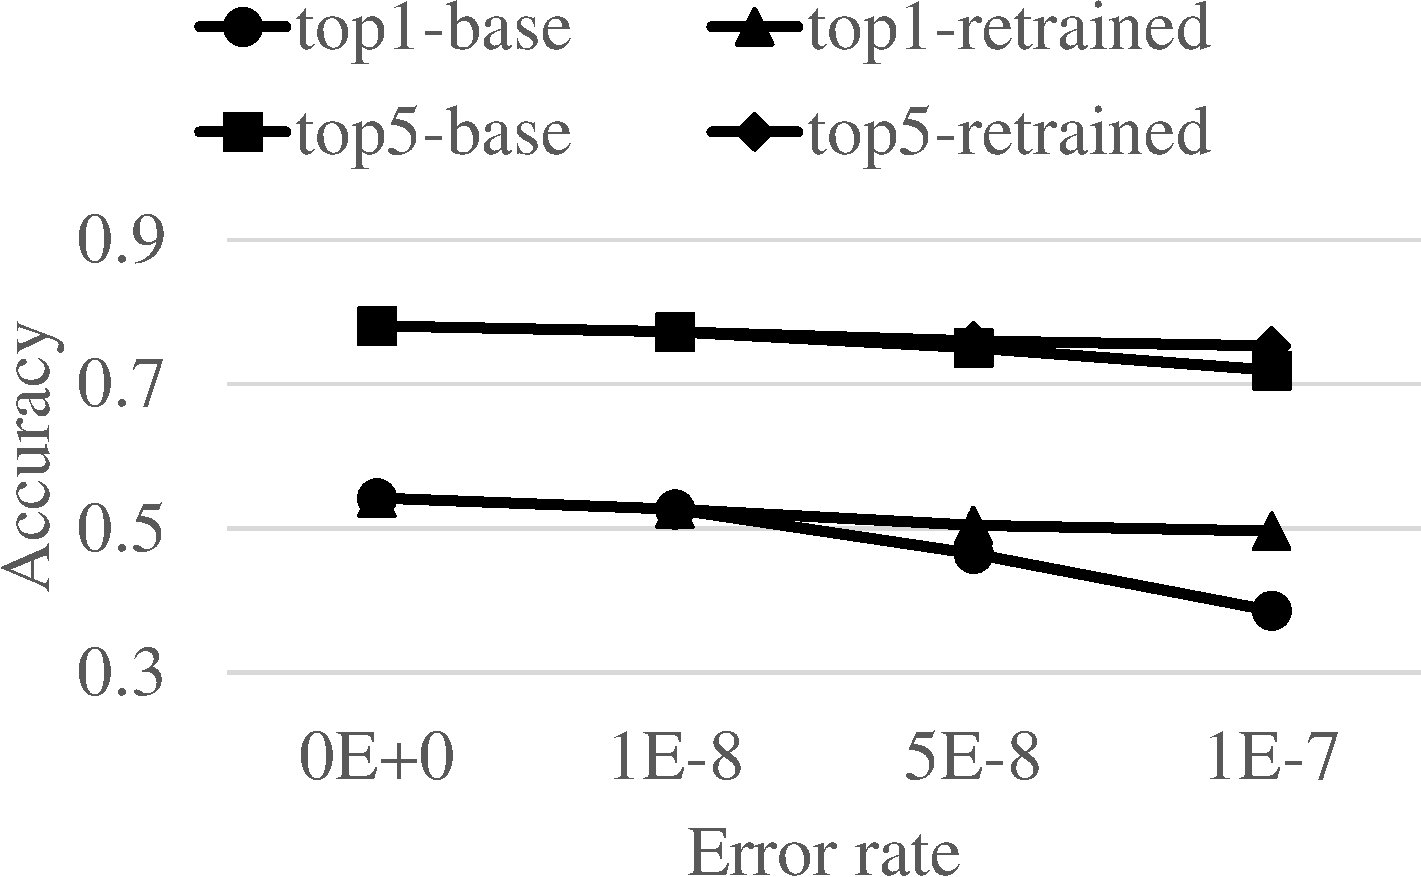
\includegraphics[width=0.7\linewidth]{alexnet-softerror}
        }
        \qquad
        \subfloat[VGG-16]{
                \label{fig:vgg16}
                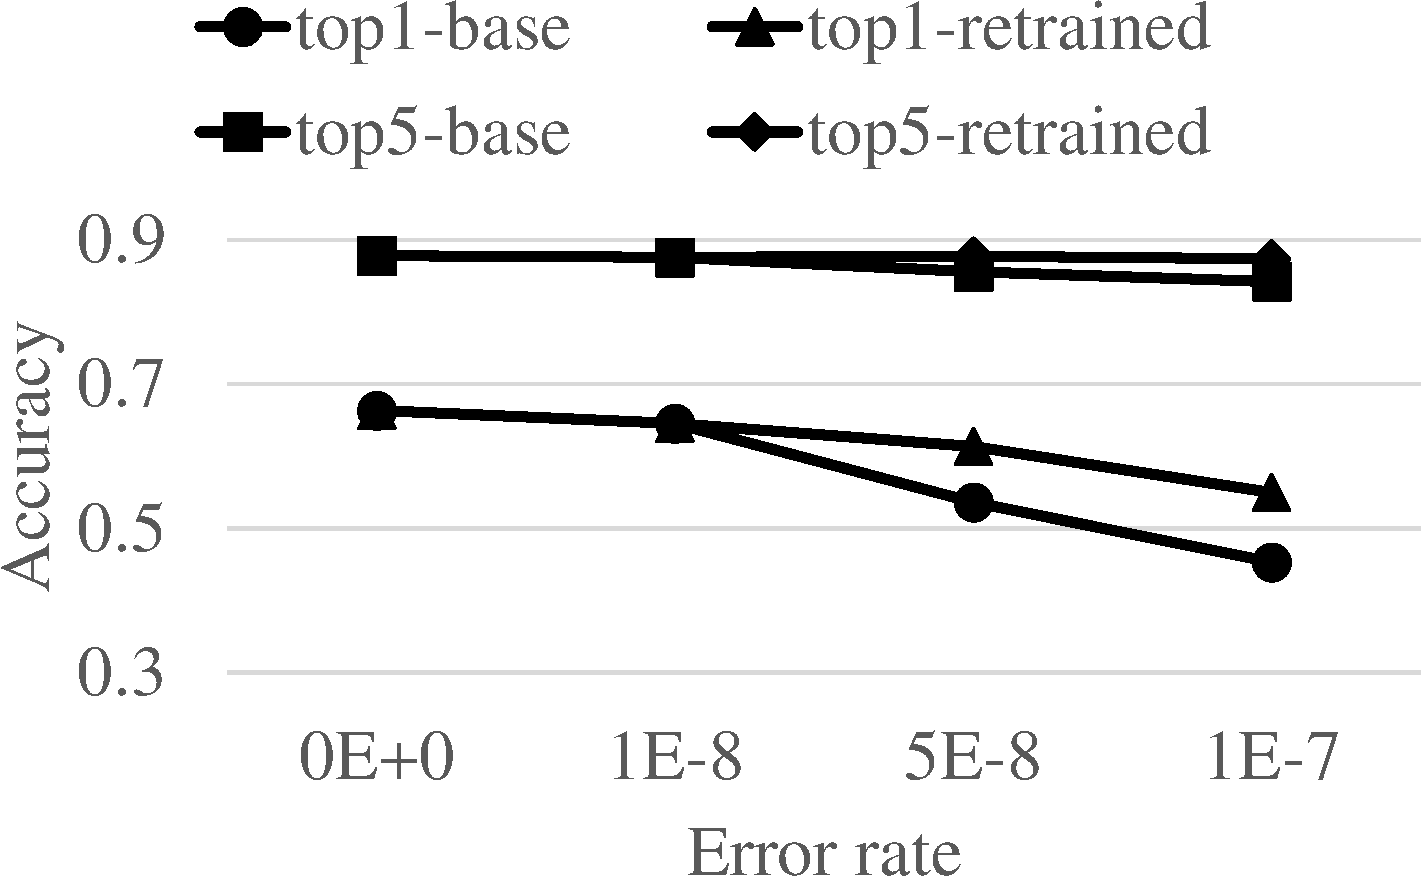
\includegraphics[width=0.7\linewidth]{vgg16-softerror}
        }
        \qquad
        \subfloat[VGG-19]{
                \label{fig:vgg19}
                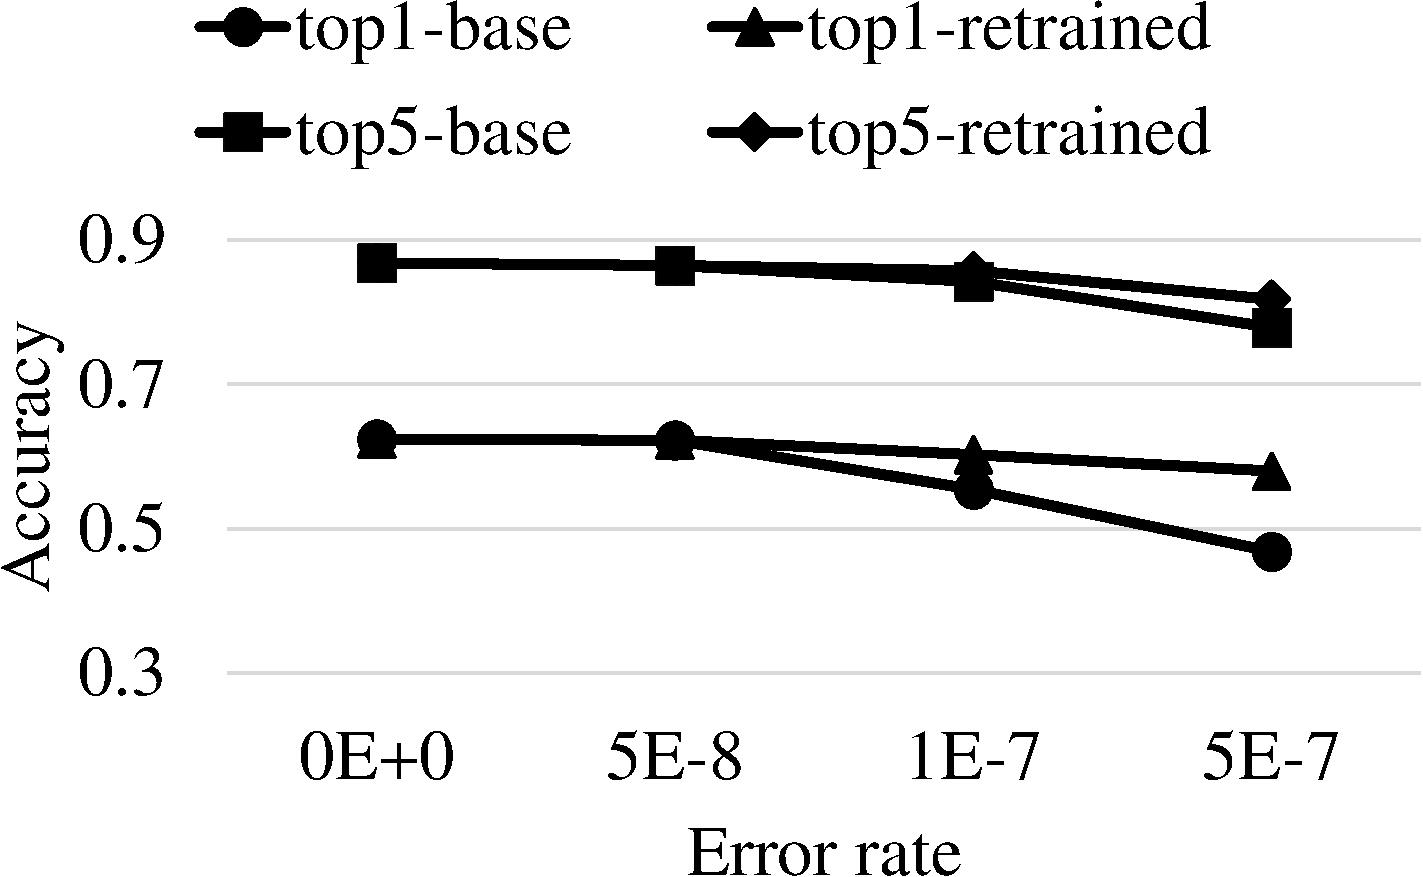
\includegraphics[width=0.7\linewidth]{vgg19-softerror}
        }
        \caption{The precision accuracy of the benchmark neural network models on accelerators with different computing errors}
        \label{fig:softerror-accuracy}
\end{figure}

\begin{figure}
        \center{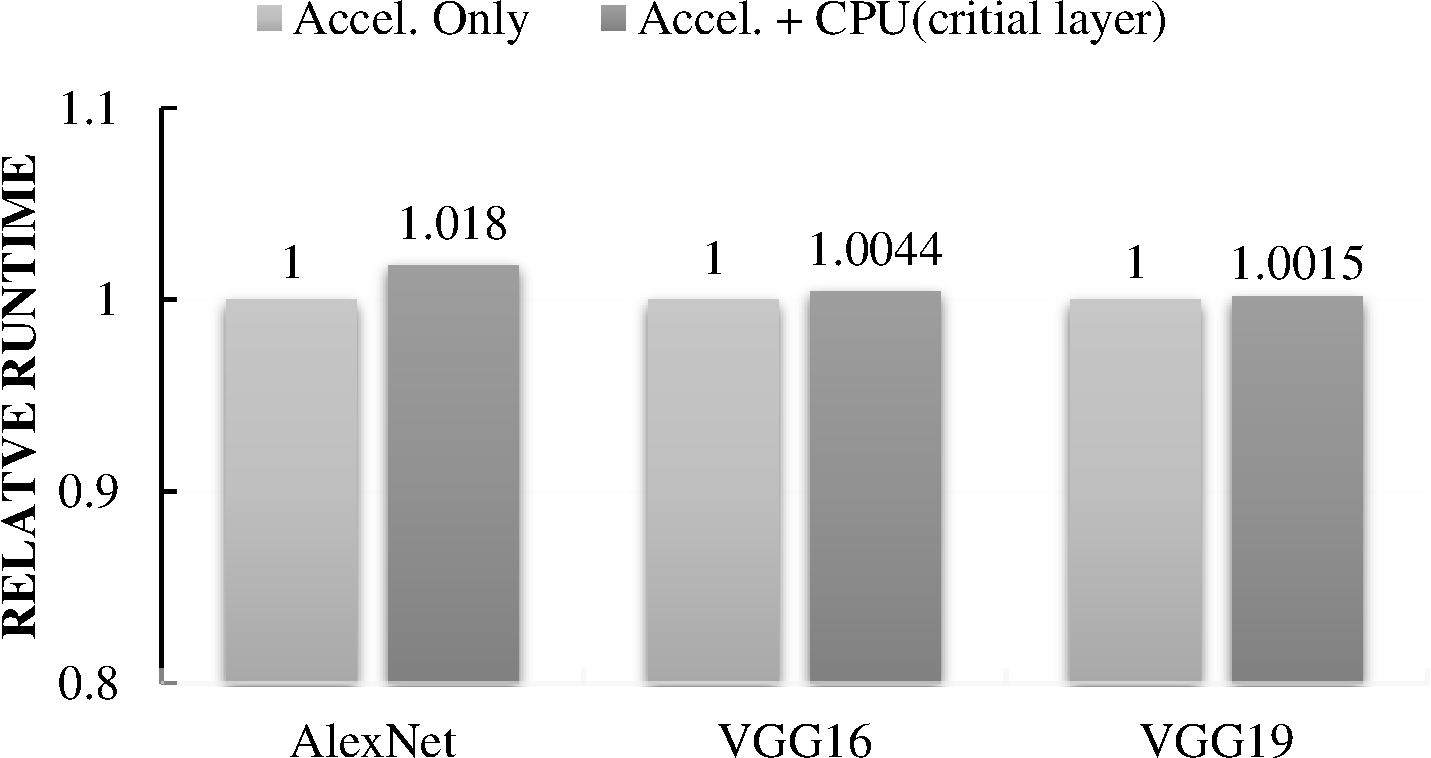
\includegraphics[width=0.7\linewidth]{clp_time}}
        \caption{Relative runtime of neural networks when the critical layer is scheduled to CPU.}
        \label{fig:clp_perf}
\end{figure}

We decide the critical layers using the error distribution as shown in Figure \ref{fig:clp_perf}.
We set the error threshold to be 5 and the experiment reveals that the last FC 
layer has the largest portion of computing errors that are more than 5. Thus, it is considered as 
the most critical layer. The critical layer takes only a small portion of the overall 
neural network computing, so the performance penalty is small even 
when it is scheduled to CPU. The last FC layer in AlexNet takes up higher portion of computing, 
the performance penalty is relatively higher compared to VGG16 and VGG19.
\begin{figure*}
        \center{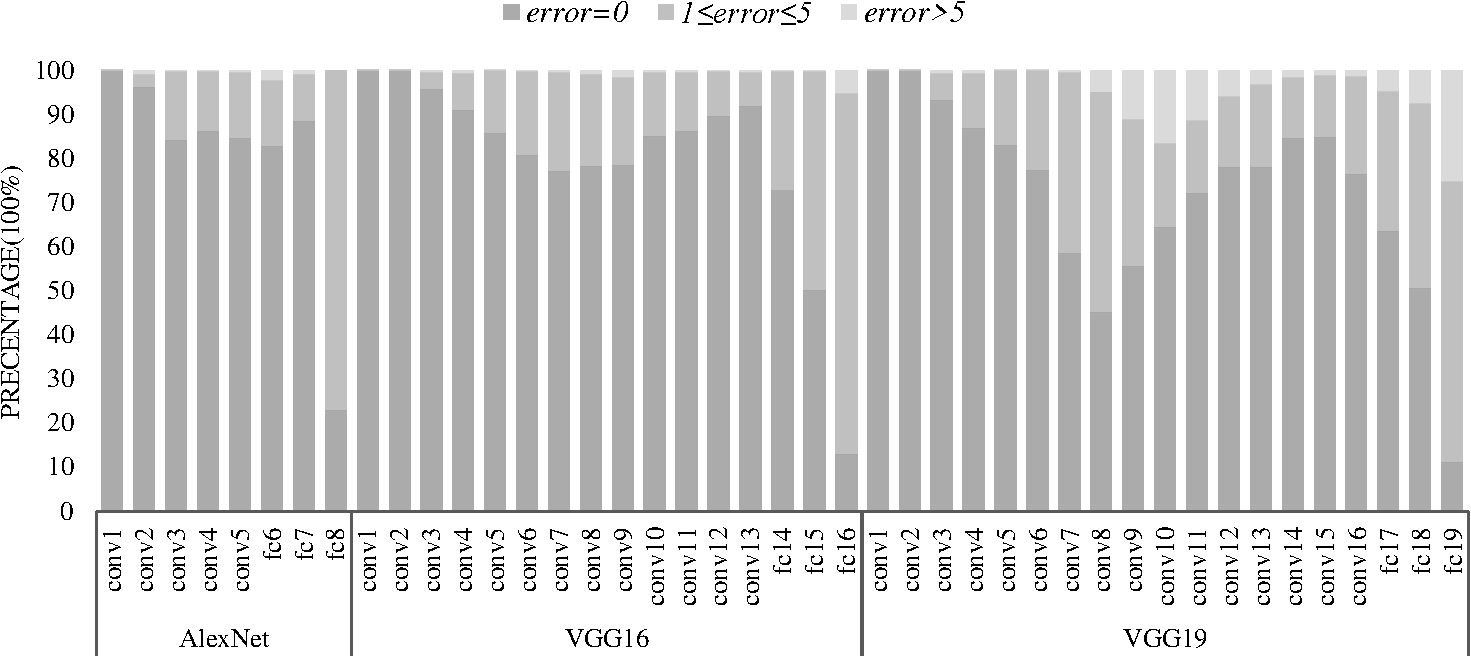
\includegraphics[width=0.8\linewidth]{error_distribute_softerror}}
        \caption{Error distribution across the neural network layers when highest BER is used in AlexNet, VGG16 and VGG19.}
        \label{fig:clp_perf}
\end{figure*}

\subsection{Overclocking case study}
To verify the proposed resilient training, we take overclocked CNN accelerator on KCU1500 as a case 
study in this work. By relaxing the timing constraints, the CNN accelerator can 
run at higher clock frequency with timing violations and computing errors. In PipeCNN, the 
hardware implementation is related to the neural network. For AlexNet, VGG16 and VGG19, the 
default implementation frequency is 210 MHz, 190 MHz and 190 MHz respectively. We then apply overclocking 
on the implementations with 10MHz step. The frequency can be boosted to 
260 MHz MHz, 240 MHz MHz and 240 MHz at most. By retraining the original neural network with 
the proposed approach, the prediction accuracy improvement is evaluated in detail.

With the overclocked CNN accelerators, we compare both the offline 
training and the proposed resilient training as presented in Figure \ref{fig:overclock-accuracy}. 
The prediction accuracy remains unchanged at the beginning and exhibits cliff-like drop 
at a tipping point. Beyond the tipping point, the prediction is no longer interesting 
due to the extremely low accuracy. At the tipping point, the top1 and top5 prediction accuracy of the 
retrained neural networks improves by xxx and xxx respectively.

\begin{figure}
        \center
	\subfloat[AlexNet]{
                \label{fig:alexnet}
                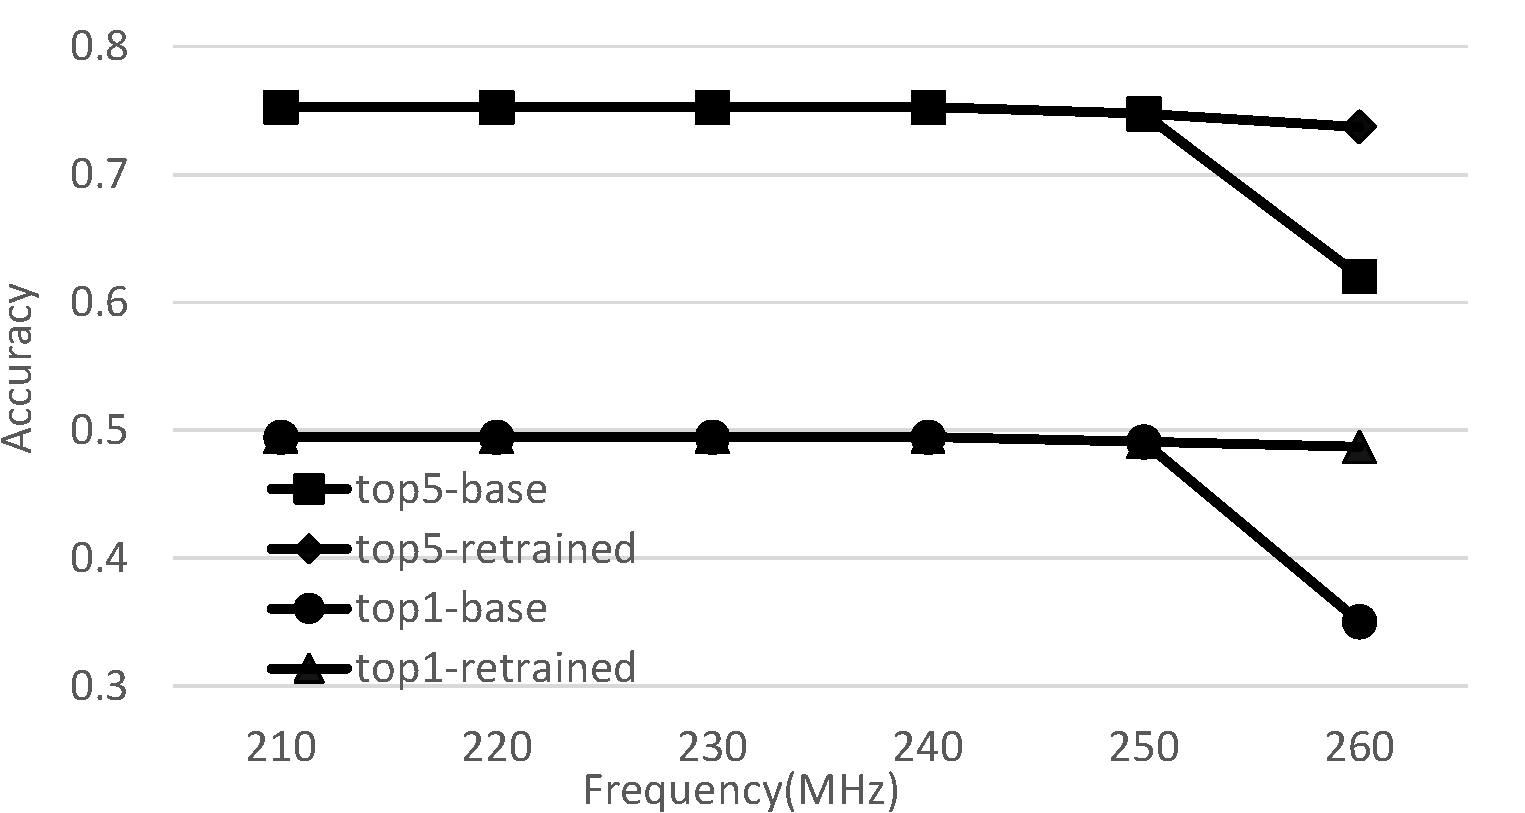
\includegraphics[width=0.6\linewidth]{alexnet-overclock}
        }
	\qquad
	\subfloat[VGG-16]{
                \label{fig:vgg16}
                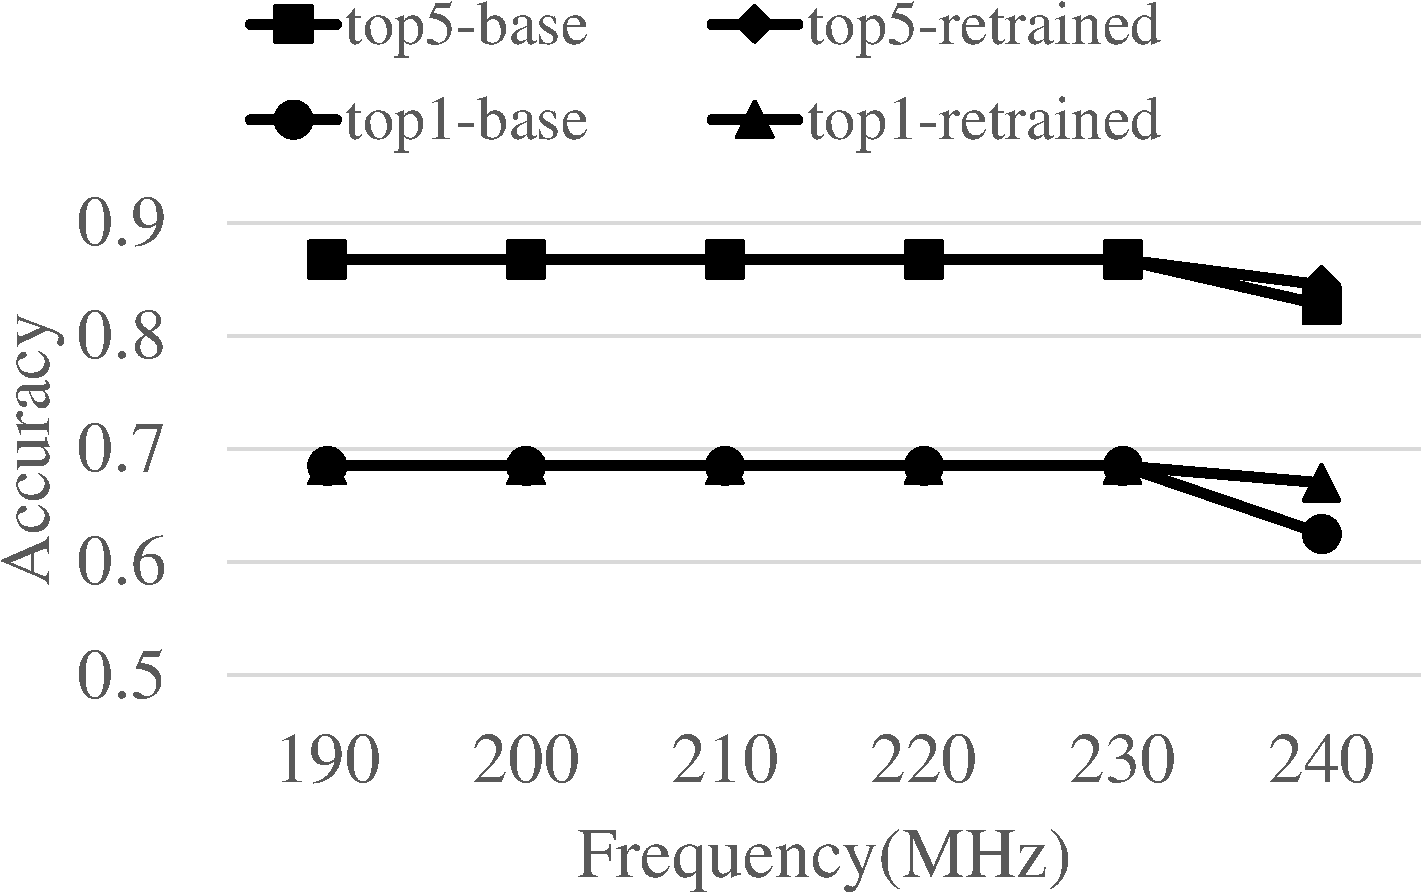
\includegraphics[width=0.6\linewidth]{vgg16-overclock}
        }
        \qquad
	\subfloat[VGG-19]{
                \label{fig:vgg19}
                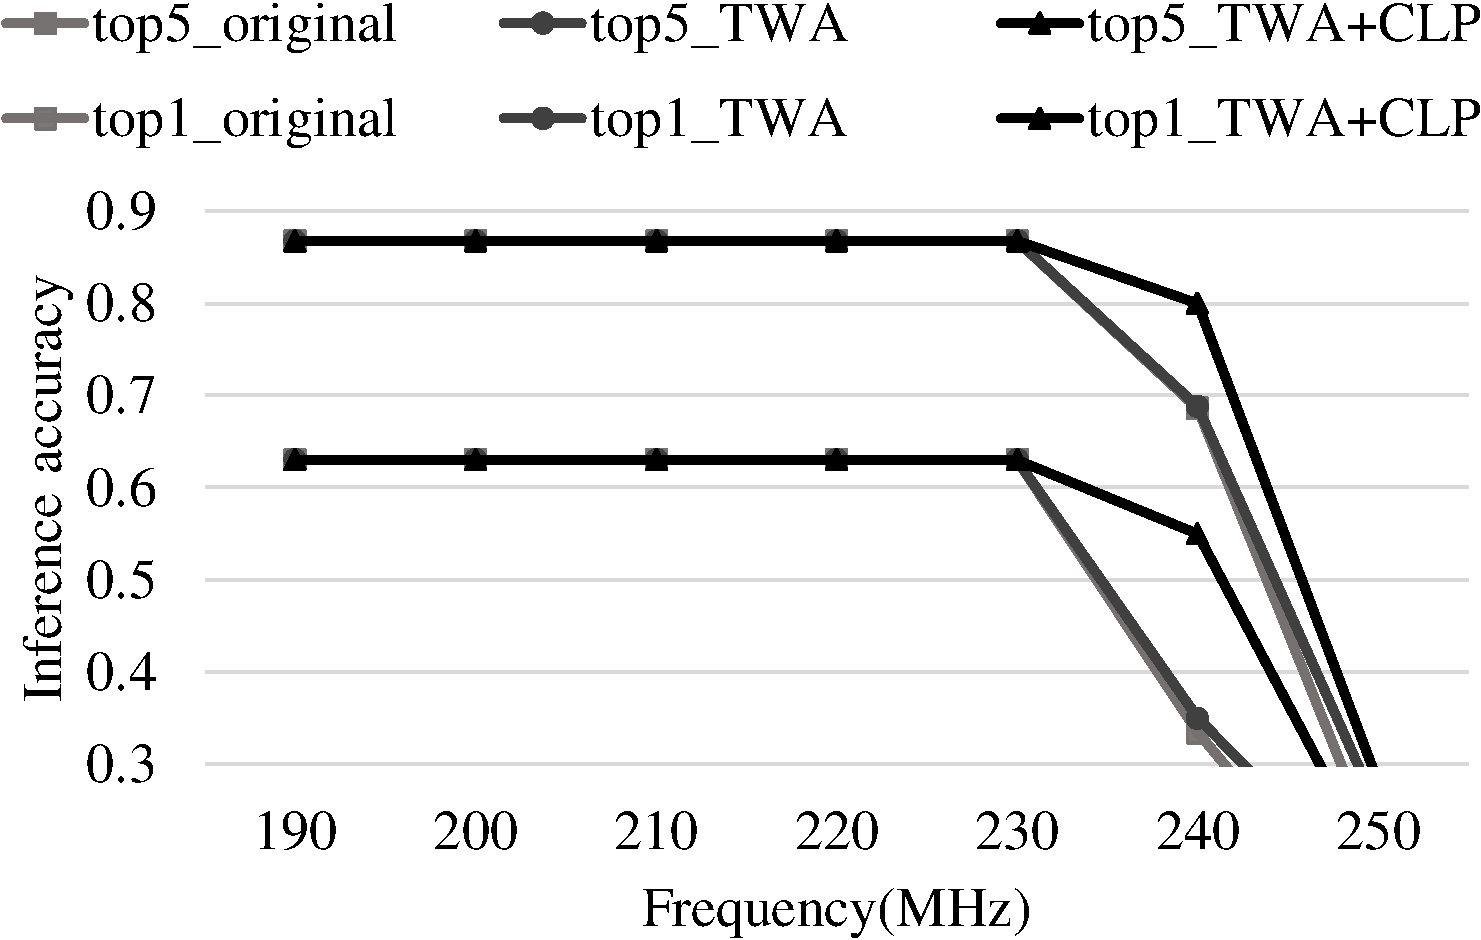
\includegraphics[width=0.6\linewidth]{vgg19-overclock}
        }
	\caption{The prediction accuracy of the benchmark neural networks on accelerators with different overclocking}
        \label{fig:overclock-accuracy}
\end{figure}

Clock frequency is almost proportional to the performance of the CNN accelerator 
especially for large convolution operation which is typically computing bound. 
Figure \ref{fig:overclocking-time} shows the relative inference runtime of the three neural networks at different 
overclocking. On the tipping point which is also the extreme overclocking case, 
the runtime improves by xxx compared to the models running on normal accelerator with 
xxx top1 accuracy loss and xxx top5 accuracy loss on average. 
\begin{figure}
        \center{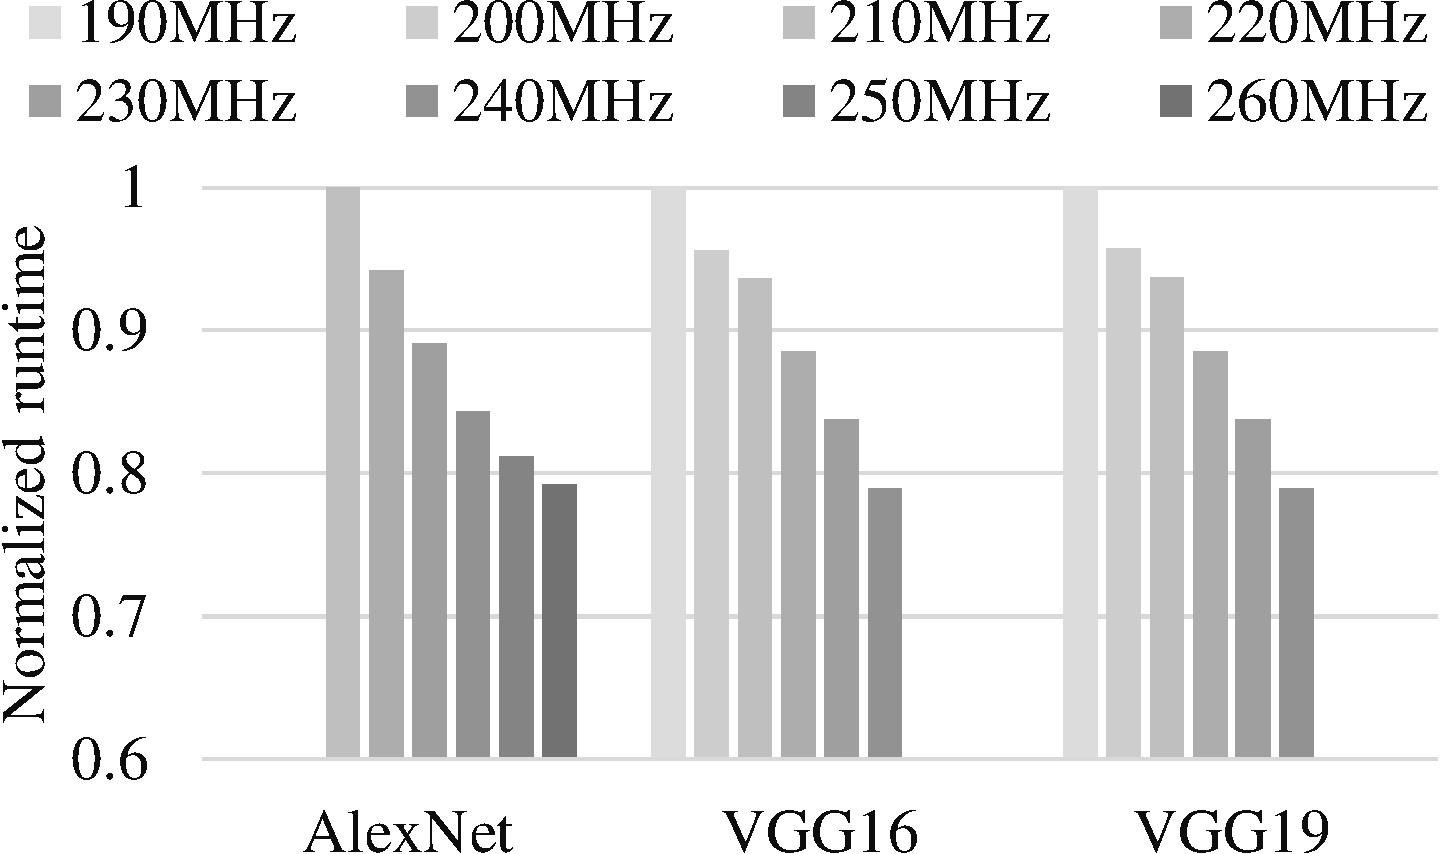
\includegraphics[width=0.6\linewidth]{relative-runtime}}
        \caption{Relative runtime of the neural networks on CNN accelerators with different overclocking. Note that AlexNet runs from 210 MHz to 250 MHz while 
		VGG16 and VGG19 ranges from 190 MHz to 240MHz, so some of the data is left blank.}
        \label{fig:overclocking-time}
\end{figure}

Comparing the experiments with random error simulation and overclocking on realistic FPGAs, we
find that the computing errors may not be uniformly distributed. In the overclocking,  
the prediction accuracy drops with cliff-like style. It indicates the computing errors may 
be quite small with light overclocking, but the amount of errors explodes at certain point.
Fortunately, the general trend is similar and the proposed training produces more resilient 
neural networks. 



As a case study to illustrate how an FPGA overlay works in practice, the design and implementation of the research project QuickDough will be examined in this section.

%%%%%%%%%%%%%%%%%%%%%%%%%%%%%%%%%%%%%%%%%%%%%%%%%%%%%%%%%%%%%%%%%%%%%%%%
% BEGIN QUICKDOUGH.TEX
%%%%%%%%%%%%%%%%%%%%%%%%%%%%%%%%%%%%%%%%%%%%%%%%%%%%%%%%%%%%%%%%%%%%%%%%
%%%
%%
%%
%%
%\section{QuickDough}
In short, QuickDough is a nested loop accelerator generation framework that is able to produce hardware accelerators rapidly~\cite{Lin:2012:EDC:2460216.2460227,Liu:2015:FSP}.
Given a user-designated loop for acceleration, QuickDough automatically generates and optimizes the corresponding hardware accelerator and its associated data I/O facilities with the host software (\figref{fig:qd_overview}).



\begin{figure}
\centering
\includegraphics[width=0.9\linewidth]{qd_overview}
\caption{QuickDough takes a user-designated loop as input and generate the corresponding hardware accelerator system using a soft coarse-grained reconfigurable array overlay.}
\label{fig:qd_overview}
\end{figure}

The overall design goal of QuickDough is to enhance designer's productivity by greatly reducing the hardware generation time and by providing automatic optimization of the data I/O between the host software and the accelerator.
Instead of spending hours on conventional hardware implementation tools, QuickDough is capable of producing the targeted hardware-software system in the order of seconds.
By doing so, it provides a rapid development experience that is compatible with that expected by most software programmers.

To achieve this compilation speed, while maintaining a reasonable accelerator performance, QuickDough avoids the creation of custom hardware directly for each application.
Instead, the compute kernel loop bodies are scheduled to execute on a CGRA overlay, which is selected from a library of pre-implemented hardware library.
By sidestepping the time-consuming low-level hardware implementation tool flow, the time to implementing an accelerator in QuickDough is reduced to essentially just the time spent on overlay selection and scheduling compute operations on the resulting overlay.
In addition, taking advantage of the overlay's softness and regularity, QuickDough allows users to perform tradeoff between compilation time and performance by selecting and customizing the overlay on a per application basis.  The result is a unified design framework that seamlessly produces the entire hardware-software infrastructure with a design experience similar to developing conventional software.

Through these facilities and through carefully partitioning the design process, QuickDough strives to improve design productivity of software programmers utilizing FPGA accelerators in 3 aspects:

\begin{enumerate}[nosep]
\item It automates most of the hardware accelerator generation process, requiring only minimum input from the application designer;
\item It produces functional hardware designs at software compilation speed (order of seconds), greatly increasing the number of debug-edit-implement cycles per day achievable;
\item It allows software programmers to progressively improve performance of the generated accelerator through subsequent optimization phases, essentially separating the functional verification and optimization process of application development.
\end{enumerate}

In the following subsections, an overview of QuickDough is presented to illustrate how it achieves the above goals.  For details, please refer to ~\cite{Lin:2012:EDC:2460216.2460227,Liu:2015:FSP}.

\subsection{Generation Framework}
\figref{fig:framework} shows an overview of the QuickDough compilation flow.
The key to rapid accelerator generation in QuickDough is to partition the complex hardware-software compilation flow into a fast and a slow path. 

\begin{figure}
    \center{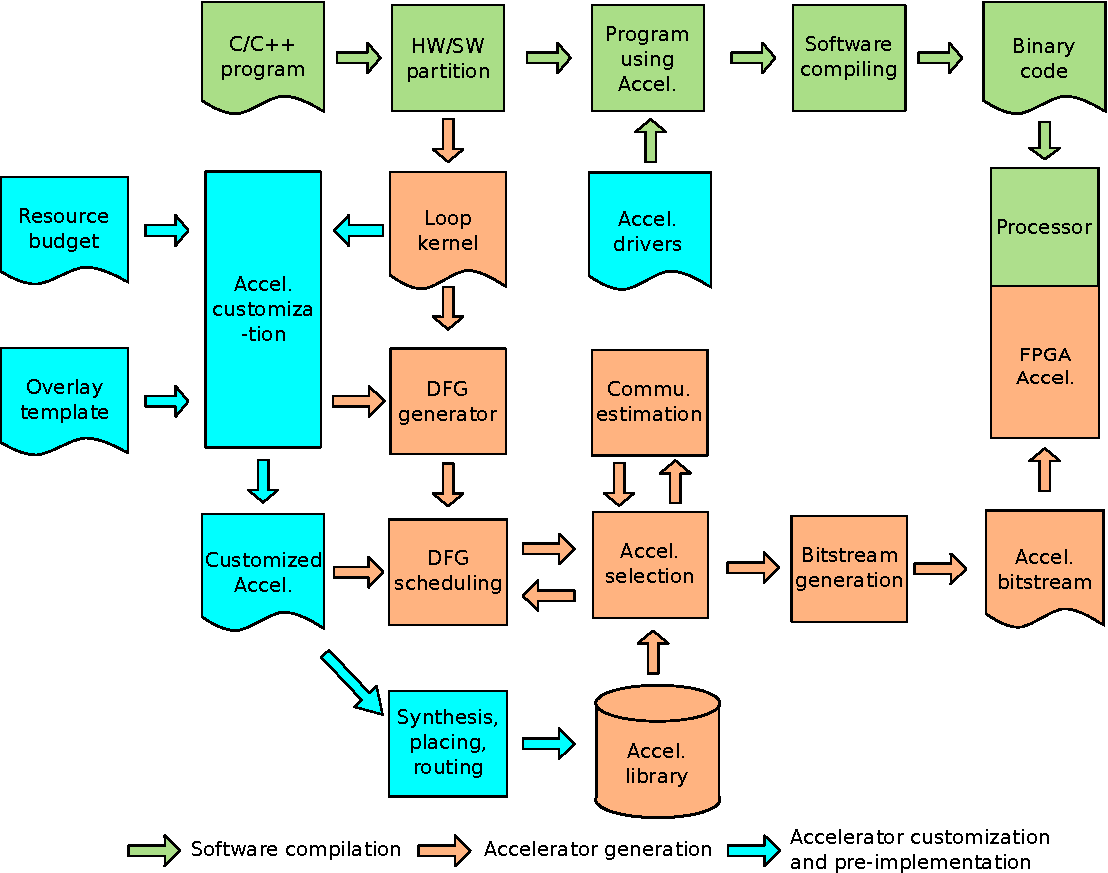
\includegraphics[width=0.8\linewidth]{quickdough_framework}}
    \caption{QuickDough: FPGA loop accelerator design framework using 
        SCGRA overlay. The compute intensive loop kernel of an 
        application is compiled to the SCGRA overlay based FPGA
    accelerator while the rest is compiled to the host processor.}
    \label{fig:framework}
\end{figure}

The fast path of QuickDough consists of the steps necessary to generate a \emph{functional} loop accelerator, which are shown in orange for hardware and in green for software generation in \figref{fig:framework}.
To begin generating a loop accelerator, QuickDough first partially unroll the compute kernel loop and extract the loop body into its corresponding data flow graph (DFG).
Subsequently, a suitable overlay configuration is selected from the pre-built implementation library on which the DFG is scheduled to execute.
Optionally, the user may choose to iteratively refine the selection by feeding back scheduling performance and estimated communication cost at each iteration.
The selected pre-built overlay implementation is then updated with the corresponding scheduling result to create the final FPGA configuration bitstream.
Finally, this updated bitstream is combined with the rest of the software to form the final application that will be executed on the target CPU-FPGA system. 

While there may seem to be a lot of steps involved in this fast path, all of them run relatively quickly.
Furthermore, the only loop in this compilation flow is the accelerator selection process, which as explained is an optional step that can be bypassed if the user opts for speed over quality.
The result is that the run time of this fast path can be kept within the order of tens of seconds.
It allows users to perform rapid design iterations, which is particularly important during early application development phases.

On the other hand, the slow path of QuickDough consists of all the remaining time-consuming steps in the flow from \figref{fig:framework}.
These steps are responsible for implementing the overlay in hardware, optimizing the CGRA to the user application, and updating the overlay library as needed.
Although these steps are slow, they are not necessarily by run for every design compilation.
For example, running through the low-level FPGA implementation is a slow process, however, they are needed only when a new overlay configuration is required.
If a compatible overlay configuration already exists in the pre-built overlay library, then the user may choose to reuse the existing implementation during early developments to facilitate fast design turn-around.
When the user decides that she is ready to spend time optimizing the overlay configuration, she may then instruct QuickDough to execute these slow steps.  With the slower steps, QuickDough will then be able to analyze the user application requirement, customize the overlay accordingly, and finally generate the FPGA configuration bitstream.
Once this bitstream is stored in the overlay library, the user will not need to go through these slow process again.

Throughout the entire application development cycle, most of the time the user will be able to execute only the fast steps, and run through the slow steps only occasionally.
As a result, the overlay compilation speed remains orders of magnitude better than traditional hardware design flow on average.

\subsection{The QuickDough Overlay}
\figref{fig:qd_overlay} shows an overview of the QuickDough overlay together with its data I/O infrastructure.
The QuickDough overlay as shown in the right hand side consists of an array of simple processing elements (PEs) connected by a direct network.
Each PE computes and forwards data to their neighbors synchronously according to a static schedule.
This schedule is stored in the instruction ROM associated with each PE and controls the action of each PE's action in every cycle.
Finally, each PE contains a scratchpad data memory for run-time data that may be reused in the same PE or be forwarded in subsequent steps.

\begin{figure}
    \center{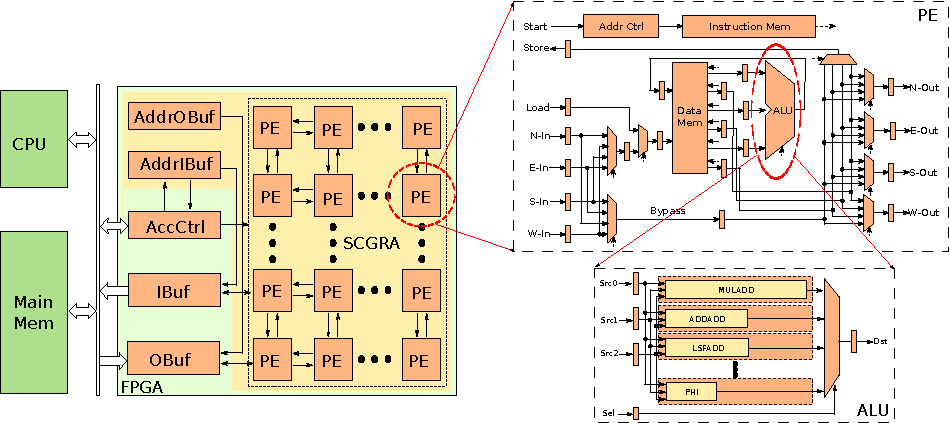
\includegraphics[width=\linewidth]{qd_overlay}}
    \caption{Overview of the QuickDough generated system.  Implemented on the FPGA is the QuickDough overlay, which is an array of PEs connected with a direct network, and the communication infrastructure with the host.}
    \label{fig:qd_overlay}
\end{figure}

Communication between the accelerator and the host processor is carried through a pair of input/output buffers.
Like with the rest of the PE array, accesses to these I/O buffers from the array also take place in lock step with the rest of the system.
The location to access in each cycle is controlled by a pair of address buffers, which contains address information generated from the QuickDough compiler. 

\figref{fig:qd_overlay} also shows the connection within a processing element.
Each PE is constructed surrounding an ALU, with multiplexors connecting the input/output of the ALU to either the internal memory or the neighboring PEs.
In this particular version, the optional load/store path is also shown, which is presented only at dedicated PE connected to the I/O buffer.
Within the PE, the ALU is supported by a multi-port data memory and an instruction memory.
Three of the data memory's read ports are connected to the ALU as inputs, while the remaining ports are sent to the output multiplexors for connection to neighboring PEs and the optional store path to output buffer (\texttt{OBuf}) external to the PE.
At the same time, this data memory takes input from the ALU output, data arriving from neighboring PEs, as well as from the optional loading path from the data input buffer (\texttt{IBuf}).

The ALU itself has a simple design that supports up to 16 fully pipelined operations.
It is constructed also as a template and may be customized to support any user-defined 3-input operations.
Regardless of its function, each operation must have a deterministic pipeline depth.
With that, the QuickDough scheduler will ensure there is never any output conflict and allow the operations to execute in parallel as needed.

Finally, note that the overlay is designed as a soft template.
Many parameters of the overlay, including the SCGRA array size, I/O buffer size, as well as the operations supported by the ALU, are configurable.
They can be optimized for a particular group of application upon user's request as part of the framework's customization steps.






\subsection{Loop Accelerator Generation}
As mentioned, an important goal of QuickDough is to generate high-performance FPGA accelerator systems in software compilation speed.  In this subsection, we will walk through some of the major steps involved and explore the details on how they help generate hardware accelerators very efficiently.


\subsubsection{DFG Generation}
The top-level inputs to QuickDough are loops that the user has designated for acceleration.
To accelerate a loop, the straightforward way is to treat each loop iteration as an individual acceleration target and rely on the host processor for loop control.
However, it is not ideal because (i) the overhead for data and control transfer between the host and FPGA will be too high, (ii) the amount of parallelism encapsulated in a single iteration of the loop body is likely to be too low for acceleration, and (iii) there will be no data reuse between loop iterations to amortize the transfer overhead between the host and the FPGA.

Therefore, just like most other acceleration frameworks, QuickDough begins the accelerator generation process by partially unrolling the input loop $U$ times to increase the amount of parallelism available.
The body of this partially unrolled loop subsequently forms the basic unit $B$ for acceleration in later steps.
This is the unit that is implemented on the FPGA accelerator using the SCGRA overlay.
With a single copy of $B$ implemented in the accelerator, the original loop is completed by executing the accelerator $N/U$ times, where $N$ is the original loop bound.

Furthermore, to amortize the communication cost between the host processor and the accelerator, input/output data are transferred in groups for $G$ invocations unit $B$ as shown in \figref{fig:blocking-and-dfg-gen}.
By buffering I/O and intermediate data on the accelerator, this grouping strategy also allow reusing data between loop iterations, further enhancing performance.

\begin{figure}
\center{\includegraphics[width=0.75\linewidth]{dfg-gen}}
\caption{Loop execution on an SCGRA overlay based FPGA accelerator}
\label{fig:blocking-and-dfg-gen}
\end{figure}

In our current implementation, the unrolling factor $U$ is specified by the user, while the grouping factor $G$ is determined by the framework automatically.
$G$ is determined based the on-chip buffer size

At the end of this process, the unrolled loop body $B$ will form the core of the accelerator and the corresponding data flow graph (DFG) will be extracted, which will drive the rest of the generation flow.



\subsubsection{Accelerator Selection}
As an accelerator generation framework, an important task of QuickDough is without doubt to generate the physical implementation of the accelerator on the FPGA.
With its SCGRA serving as an intermediate layer, this translates into physically implementing the overlay on the FPGA.
Unfortunately, no matter how simple the overlay is, running through the low-level hardware implementation tools is going to be a lengthy process, contradicting the original goal of employing the overlay in the first place.
In order to sidestep this lengthy hardware implementation process, QuickDough instead transform it into a selection process from a library of pre-implemented overlay.

When compared to directly implementing the overlay using standard hardware implementation tools, this accelerator selection process is much faster.
In return, the performance of the resulting overlay configuration may not be optimal for the given user application.
Despite the suboptimal performance, the selected overlay implementation is functionally correct and should give a good sense of the overall hardware-software codesign process to the software programmer, which is necessary for rapid early development.
The user may subsequently opt for the slower optimization and customization steps explained in the next subsection to progressively improve performance.

As such, the goal of this process is to select the \emph{best} and \emph{functional} overlay configuration from the pre-implemented library \emph{rapidly}.
While functionality is easy to determine, QuickDough must also be able to estimate the resulting performance swiftly for this selection process.
Now, the performance of the accelerator depends mainly on two factors: (i) computational latency, and (ii) communication latency.
As the SCGRA overlay is regular and computes with a deterministic schedule, its exact computational latency of carrying out the user DFG can readily be obtained from the scheduler.
Of all the configurable parameters of the overlay, the SCGRA array size is the dominant factor affecting this computational latency.
On the other hand, communication latency depends not only on the scheduling results, but also other factors such as communication pattern, grouping factor, I/O buffer sizes, as well as DMA transfer latency, etc.
These parameters interact with each other to form a large design space.
For rapid estimation, instead of performing a full design space exploration, QuickDough is able to rely on simple analytical model for estimating communication latency based on the overlay SCGRA array size.

Finally, QuickDough leaves this choice of effort in finding the best accelerator configuration to the user as 3 optimization effort levels:
\begin{itemize}[nosep]
\item Level 0 (\texttt{O0}) -- No optimization.  QuickDough selects a feasible accelerator configuration with the smallest SCGRA size.
\item Level 1 (\texttt{O1}) -- QuickDough estimates performances of 3 accelerators with different array sizes and select the one that results in the best performance.
\item Level 2 (\texttt{O2}) -- QuickDough performs an exhaustive search on all accelerators in the library and searches for the best accelerator configuration. 
\end{itemize}

Obviously, the more effort is being put into the selection process, the longer the process will take, and the resulting performance is improved most of the time.
The choice on how much effort to pay is up to the user.

\subsubsection{DFG Scheduling}
This is the step where the DFG extracted from the unrolled loop body is scheduled to execute on the selected SCGRA overlay.
For each operation in the DFG, the scheduler must decide the cycle and the PE in which the operation should be carried out.
The scheduler also determines the routing of data between the producing and consuming PEs, as well as to/from the I/O buffer.

As QuickDough tends to target DFGs with close to thousands of node, to keep the scheduling time short, a classical list scheduling algorithm was adopted~\cite{schutten1996list}.
A scheduling metric proposed in~\cite{Lin:2012:EDC:2460216.2460227} that considers both load balancing and communication cost was used in the scheduler.

At the end of this scheduling step, a schedule with operation of each PE and data I/O buffer in every cycle is produced.
This schedule essentially turns the generic overlay implementation into the specific accelerator for the user application.


\subsubsection{Accelerator Bitstream Generation}
The final step of the accelerator generation process is to produce the instructions for each PE and the address sequences for the I/O buffers according to the scheduler's result.

As a way to reduce area overhead of the overlay, both the instruction memory of each PE as well as the I/O address buffers are implemented as read-only memories (ROMs) on the physical FPGA.
To update the content of these memories, the QuickDough framework must update the FPGA implementation bitstream directly.
%
To do that, the memory organization and placement information of the target overlay implementation is obtained from an \code{XDL} file corresponding to the overlay implementation \cite{beckhoff2011xilinx}.
The resulting memory organization information is encoded in the corresponding \code{BMM} file, which is combined with the scheduler results to update the overlay implementation bitstream with the the \code{data2mem} tool from Xilinx \cite{data2mem}.

While it may sound complicated, the whole process is automated and consumes only a few seconds of tools run time.
The result of this process is an updated bitstream with all application-specific instructions embedded.
This updated bitstream is the final configuration file used to program the physical FPGA, and it concludes the QuickDough flow.


\subsection{Customization \& Optimization}
The true power of utilizing an FPGA overlay rests on that fact that the overlay is virtual, soft, and easily customizable for the need of the application.
In this part, we will examine various ways QuickDough enables user to customize and optimize the overlay to improve power-performance of the generated accelerators.
Unlike the fast generation path explained above, these customization steps are much more time consuming.
As such, these customization steps are considered part of the slow path in QuickDough's design philosophy, and are expected to execute only occasionally as needed.

There are a number of reasons why a user may want to spend the time on customization despite the slow process.
To begin, the user may want to construct a prebuilt implementation library specific to the target application domain. 
It is useful as the result can be memoized in the implementation library and be reused by all other target applications, amortizing the initial implementation effort.
Once the project development has gone through the initial debugging phase, a user may also opt for creating a customized overlay for the particular accelerated application.
This per-application optimization will help improve the performance of the accelerator but the process will undoubtedly be slower than to select a prebuilt implementation.
Luckily, the result of this per-application customization can be stored in the prebuilt library such that it can be reused on subsequent compilations.

\subsubsection{What can be customized?}
For the purpose of customization, the QuickDough overlay was designed from the beginning to be a template from which a family of overlay instances could be generated.
The SCGRA overlay consists of a regular array of simple PEs connected with direct connections.
Depending on the application requirements, a range of design parameters of this overlay can then be customized, including the array size, on-chip scratchpad data memory capacity, instruction memory capacity and I/O buffer capacity.
On top of that, as a hardware-software system generator for loop acceleration, QuickDough may also optimizes the communication between the accelerator and the host software by varying the \emph{grouping factor}, which determines the amount of data transferred between the two in each transaction.
Finally, it may also optionally optimizes the \emph{loop unrolling factor} on behalf of the user depending on the computational capability of the overlay as a function of its array size.

Obviously, a major challenge when optimizing this set of parameters is that they tend to interact with one another in fairly complex ways.
For example, increasing the array size increases the compute capability of the array, potentially improving the accelerator performance.  However, the increased size is beneficial only if the input DFG has enough parallelism presented to take advantage of the increased capability.
To increase the amount of available computation, QuickDough may optionally increase the amount of loop unrolling in the user-supplied kernel.
However, that also increases the amount of data I/O required, as well as the on-chip instruction and data buffer requirement, which in turn limits the size of the array in the first place.
A full discussion of the detailed customization and optimization process is beyond the scope of this chapter.  Yet it is worthwhile to realize the potential of customization here.

As an illustration, \figref{fig:qd_customization_fir} shows the effect of customization on the generated accelerators from QuickDough.
In this example, accelerator for a 49-tap FIR filter was generated on the Zedboard using QuickDough.
Three different customized overlay configurations were generated.
Beginning with the specified array size, the rest of the configuration parameters were determined automatically. 


\begin{figure}
\centering
\subfigure[Performance]{
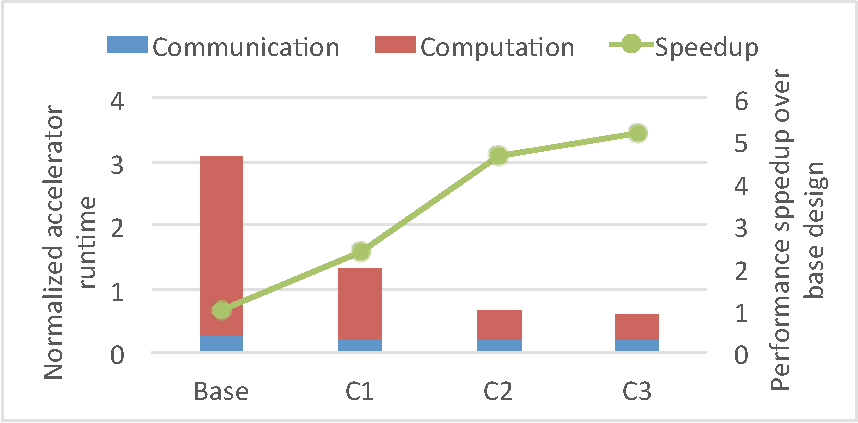
\includegraphics[width=0.47\linewidth]{qd_customization_ex}
\label{fig:qd_customization_ex}
}
\hfill
\subfigure[Resource Consumptions]{
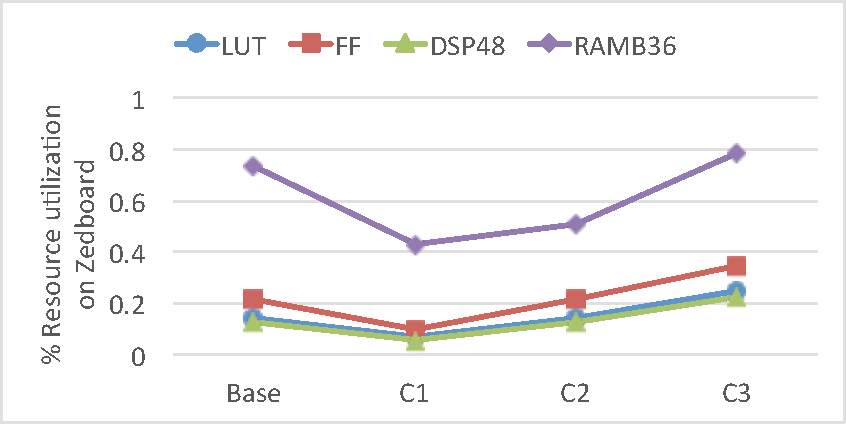
\includegraphics[width=0.47\linewidth]{qd_customization_resource}
\label{fig:qd_customization_resource}
}
\newline
\subfigure[Overlay configuration]{
\begin{minipage}{0.9\linewidth}
\centering
\footnotesize
\begin{tabular}{ccccc}
\toprule
&base&C1&C2&C3\\
\midrule
Loop unrolling factor&10$\times$50&50$\times$50&50$\times$50&50$\times$50\\
Grouping factor&100$\times$50&2500$\times$50&1250$\times$50&5000$\times$50\\
SCGRA size&3$\times$3&2$\times$2&3$\times$3&4$\times$4\\
Inst Mem Depth&4k&4k&2k&1k\\
IO Buffer Depth&1k&4k&2k&8k\\
\bottomrule
\end{tabular}
\end{minipage}
}
\caption{Effect of overlay customization on performance and resource consumption.  Example here shows the result of an FIR filter using QuickDough with 3 different overlay configurations over a base design.}
\label{fig:qd_customization_fir}
\end{figure}

A few interesting observations can be made from the figures.  In terms of performance, comparing to the sub-optimal baseline configuration, the best configuration (\textsc{c3}) results in more than 5 times improvement in performance.
Furthermore, comparing the baseline and \textsc{c2} that feature the same array size ($3\times 3$), $4.7\times$ improvement in performance can be obtained by optimizing the unrolling and grouping factor in combination with the on-chip memory configuration.
Interestingly, looking at the resource consumptions, \textsc{c2} in fact consumes $31\%$ less on-chip memory and the same resource otherwise as the baseline.

\subsection{Summary}
Using QuickDough as a case study, we have illustrated how the use of an FPGA overlay has enabled a very different experience for software programmers when designing hardware-software systems.
The 2-layer approach to hardware design allows for a very rapid design experience that sharply contrasts the lengthy low-level hardware tool flow.
Furthermore, the softness of the overlay provides opportunity for further customization and optimization as the development effort progresses.
Together, it creates for novice users a ``software-like'' way to designing complex accelerator systems while maintaining considerable overall acceleration performance promised by FPGAs.



%%
%%
%%
%%


%%
%%
%%
%%
%\section{QuickDough}
In short, QuickDough is a nested loop accelerator generation framework that is able to produce hardware accelerators rapidly~\cite{Lin:2012:EDC:2460216.2460227,Liu:2015:FSP}.
Given a user-designated loop for acceleration, QuickDough automatically generates and optimizes the corresponding hardware accelerator and its associated data I/O facilities with the host software (\figref{fig:qd_overview}).



\begin{figure}
\centering
\includegraphics[width=0.9\linewidth]{qd_overview}
\caption{QuickDough takes a user-designated loop as input and generate the corresponding hardware accelerator system using a soft coarse-grained reconfigurable array overlay.}
\label{fig:qd_overview}
\end{figure}

The overall design goal of QuickDough is to enhance designer's productivity by greatly reducing the hardware generation time and by providing automatic optimization of the data I/O between the host software and the accelerator.
Instead of spending hours on conventional hardware implementation tools, QuickDough is capable of producing the targeted hardware-software system in the order of seconds.
By doing so, it provides a rapid development experience that is compatible with that expected by most software programmers.

To achieve this compilation speed, while maintaining a reasonable accelerator performance, QuickDough avoids the creation of custom hardware directly for each application.
Instead, the compute kernel loop bodies are scheduled to execute on a CGRA overlay, which is selected from a library of pre-implemented hardware library.
By sidestepping the time-consuming low-level hardware implementation tool flow, the time to implementing an accelerator in QuickDough is reduced to essentially just the time spent on overlay selection and scheduling compute operations on the resulting overlay.
In addition, taking advantage of the overlay's softness and regularity, QuickDough allows users to perform tradeoff between compilation time and performance by selecting and customizing the overlay on a per application basis.  The result is a unified design framework that seamlessly produces the entire hardware-software infrastructure with a design experience similar to developing conventional software.

Through these facilities and through carefully partitioning the design process, QuickDough strives to improve design productivity of software programmers utilizing FPGA accelerators in 3 aspects:

\begin{enumerate}[nosep]
\item It automates most of the hardware accelerator generation process, requiring only minimum input from the application designer;
\item It produces functional hardware designs at software compilation speed (order of seconds), greatly increasing the number of debug-edit-implement cycles per day achievable;
\item It allows software programmers to progressively improve performance of the generated accelerator through subsequent optimization phases, essentially separating the functional verification and optimization process of application development.
\end{enumerate}

In the following subsections, an overview of QuickDough is presented to illustrate how it achieves the above goals.  For details, please refer to ~\cite{Lin:2012:EDC:2460216.2460227,Liu:2015:FSP}.

\subsection{Generation Framework}
\figref{fig:framework} shows an overview of the QuickDough compilation flow.
The key to rapid accelerator generation in QuickDough is to partition the complex hardware-software compilation flow into a fast and a slow path. 

\begin{figure}
    \center{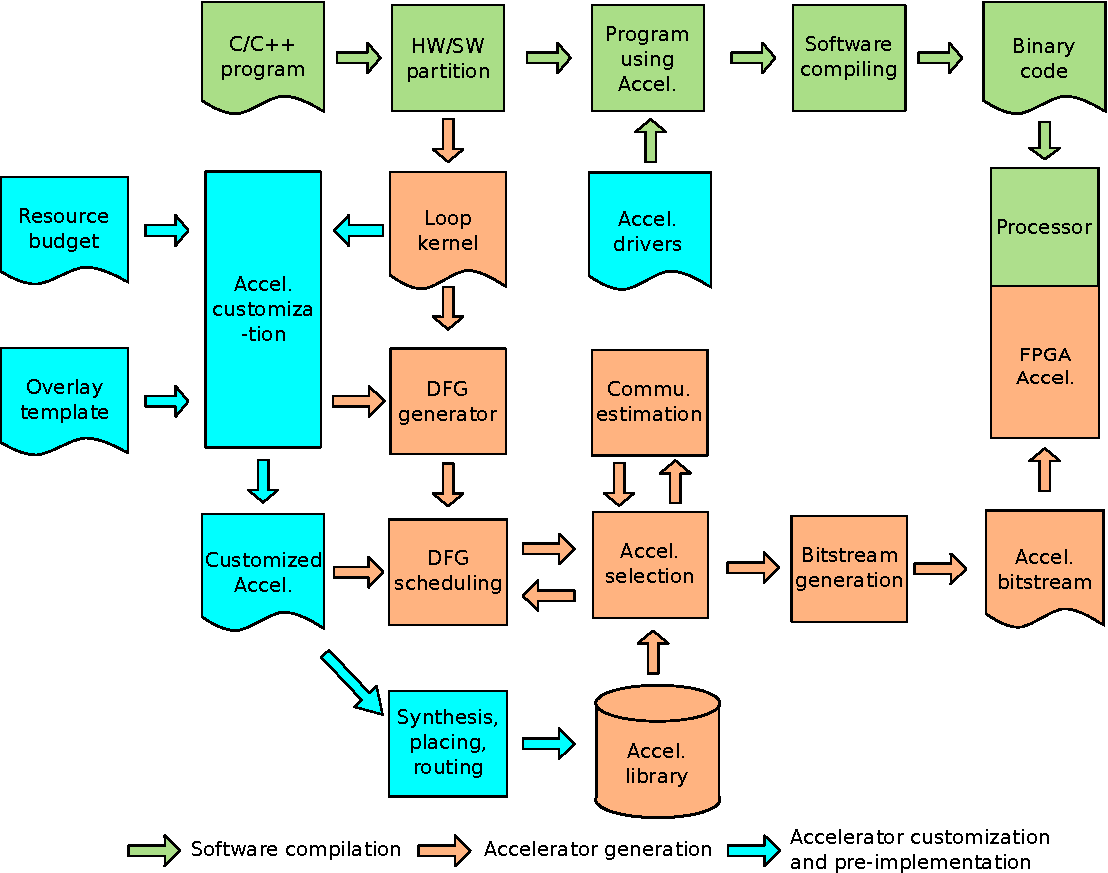
\includegraphics[width=0.8\linewidth]{quickdough_framework}}
    \caption{QuickDough: FPGA loop accelerator design framework using 
        SCGRA overlay. The compute intensive loop kernel of an 
        application is compiled to the SCGRA overlay based FPGA
    accelerator while the rest is compiled to the host processor.}
    \label{fig:framework}
\end{figure}

The fast path of QuickDough consists of the steps necessary to generate a \emph{functional} loop accelerator, which are shown in orange for hardware and in green for software generation in \figref{fig:framework}.
To begin generating a loop accelerator, QuickDough first partially unroll the compute kernel loop and extract the loop body into its corresponding data flow graph (DFG).
Subsequently, a suitable overlay configuration is selected from the pre-built implementation library on which the DFG is scheduled to execute.
Optionally, the user may choose to iteratively refine the selection by feeding back scheduling performance and estimated communication cost at each iteration.
The selected pre-built overlay implementation is then updated with the corresponding scheduling result to create the final FPGA configuration bitstream.
Finally, this updated bitstream is combined with the rest of the software to form the final application that will be executed on the target CPU-FPGA system. 

While there may seem to be a lot of steps involved in this fast path, all of them run relatively quickly.
Furthermore, the only loop in this compilation flow is the accelerator selection process, which as explained is an optional step that can be bypassed if the user opts for speed over quality.
The result is that the run time of this fast path can be kept within the order of tens of seconds.
It allows users to perform rapid design iterations, which is particularly important during early application development phases.

On the other hand, the slow path of QuickDough consists of all the remaining time-consuming steps in the flow from \figref{fig:framework}.
These steps are responsible for implementing the overlay in hardware, optimizing the CGRA to the user application, and updating the overlay library as needed.
Although these steps are slow, they are not necessarily by run for every design compilation.
For example, running through the low-level FPGA implementation is a slow process, however, they are needed only when a new overlay configuration is required.
If a compatible overlay configuration already exists in the pre-built overlay library, then the user may choose to reuse the existing implementation during early developments to facilitate fast design turn-around.
When the user decides that she is ready to spend time optimizing the overlay configuration, she may then instruct QuickDough to execute these slow steps.  With the slower steps, QuickDough will then be able to analyze the user application requirement, customize the overlay accordingly, and finally generate the FPGA configuration bitstream.
Once this bitstream is stored in the overlay library, the user will not need to go through these slow process again.

Throughout the entire application development cycle, most of the time the user will be able to execute only the fast steps, and run through the slow steps only occasionally.
As a result, the overlay compilation speed remains orders of magnitude better than traditional hardware design flow on average.

\subsection{The QuickDough Overlay}
\figref{fig:qd_overlay} shows an overview of the QuickDough overlay together with its data I/O infrastructure.
The QuickDough overlay as shown in the right hand side consists of an array of simple processing elements (PEs) connected by a direct network.
Each PE computes and forwards data to their neighbors synchronously according to a static schedule.
This schedule is stored in the instruction ROM associated with each PE and controls the action of each PE's action in every cycle.
Finally, each PE contains a scratchpad data memory for run-time data that may be reused in the same PE or be forwarded in subsequent steps.

\begin{figure}
    \center{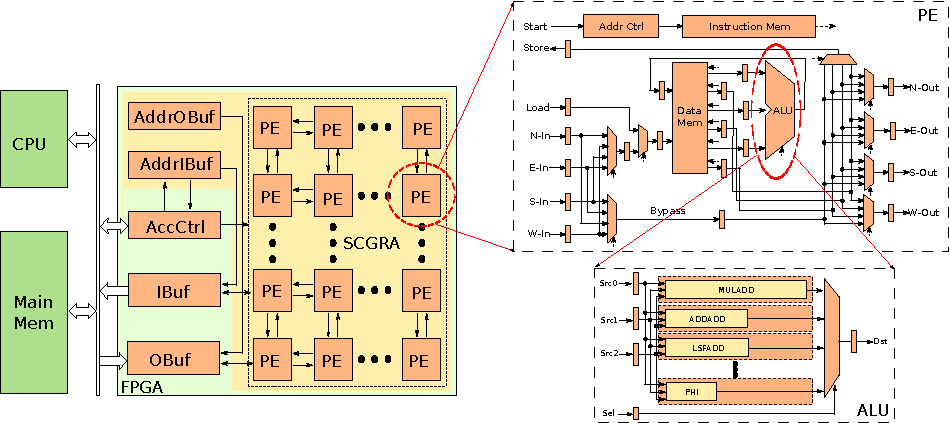
\includegraphics[width=\linewidth]{qd_overlay}}
    \caption{Overview of the QuickDough generated system.  Implemented on the FPGA is the QuickDough overlay, which is an array of PEs connected with a direct network, and the communication infrastructure with the host.}
    \label{fig:qd_overlay}
\end{figure}

Communication between the accelerator and the host processor is carried through a pair of input/output buffers.
Like with the rest of the PE array, accesses to these I/O buffers from the array also take place in lock step with the rest of the system.
The location to access in each cycle is controlled by a pair of address buffers, which contains address information generated from the QuickDough compiler. 

\figref{fig:qd_overlay} also shows the connection within a processing element.
Each PE is constructed surrounding an ALU, with multiplexors connecting the input/output of the ALU to either the internal memory or the neighboring PEs.
In this particular version, the optional load/store path is also shown, which is presented only at dedicated PE connected to the I/O buffer.
Within the PE, the ALU is supported by a multi-port data memory and an instruction memory.
Three of the data memory's read ports are connected to the ALU as inputs, while the remaining ports are sent to the output multiplexors for connection to neighboring PEs and the optional store path to output buffer (\texttt{OBuf}) external to the PE.
At the same time, this data memory takes input from the ALU output, data arriving from neighboring PEs, as well as from the optional loading path from the data input buffer (\texttt{IBuf}).

The ALU itself has a simple design that supports up to 16 fully pipelined operations.
It is constructed also as a template and may be customized to support any user-defined 3-input operations.
Regardless of its function, each operation must have a deterministic pipeline depth.
With that, the QuickDough scheduler will ensure there is never any output conflict and allow the operations to execute in parallel as needed.

Finally, note that the overlay is designed as a soft template.
Many parameters of the overlay, including the SCGRA array size, I/O buffer size, as well as the operations supported by the ALU, are configurable.
They can be optimized for a particular group of application upon user's request as part of the framework's customization steps.






\subsection{Loop Accelerator Generation}
As mentioned, an important goal of QuickDough is to generate high-performance FPGA accelerator systems in software compilation speed.  In this subsection, we will walk through some of the major steps involved and explore the details on how they help generate hardware accelerators very efficiently.


\subsubsection{DFG Generation}
The top-level inputs to QuickDough are loops that the user has designated for acceleration.
To accelerate a loop, the straightforward way is to treat each loop iteration as an individual acceleration target and rely on the host processor for loop control.
However, it is not ideal because (i) the overhead for data and control transfer between the host and FPGA will be too high, (ii) the amount of parallelism encapsulated in a single iteration of the loop body is likely to be too low for acceleration, and (iii) there will be no data reuse between loop iterations to amortize the transfer overhead between the host and the FPGA.

Therefore, just like most other acceleration frameworks, QuickDough begins the accelerator generation process by partially unrolling the input loop $U$ times to increase the amount of parallelism available.
The body of this partially unrolled loop subsequently forms the basic unit $B$ for acceleration in later steps.
This is the unit that is implemented on the FPGA accelerator using the SCGRA overlay.
With a single copy of $B$ implemented in the accelerator, the original loop is completed by executing the accelerator $N/U$ times, where $N$ is the original loop bound.

Furthermore, to amortize the communication cost between the host processor and the accelerator, input/output data are transferred in groups for $G$ invocations unit $B$ as shown in \figref{fig:blocking-and-dfg-gen}.
By buffering I/O and intermediate data on the accelerator, this grouping strategy also allow reusing data between loop iterations, further enhancing performance.

\begin{figure}
\center{\includegraphics[width=0.75\linewidth]{dfg-gen}}
\caption{Loop execution on an SCGRA overlay based FPGA accelerator}
\label{fig:blocking-and-dfg-gen}
\end{figure}

In our current implementation, the unrolling factor $U$ is specified by the user, while the grouping factor $G$ is determined by the framework automatically.
$G$ is determined based the on-chip buffer size

At the end of this process, the unrolled loop body $B$ will form the core of the accelerator and the corresponding data flow graph (DFG) will be extracted, which will drive the rest of the generation flow.



\subsubsection{Accelerator Selection}
As an accelerator generation framework, an important task of QuickDough is without doubt to generate the physical implementation of the accelerator on the FPGA.
With its SCGRA serving as an intermediate layer, this translates into physically implementing the overlay on the FPGA.
Unfortunately, no matter how simple the overlay is, running through the low-level hardware implementation tools is going to be a lengthy process, contradicting the original goal of employing the overlay in the first place.
In order to sidestep this lengthy hardware implementation process, QuickDough instead transform it into a selection process from a library of pre-implemented overlay.

When compared to directly implementing the overlay using standard hardware implementation tools, this accelerator selection process is much faster.
In return, the performance of the resulting overlay configuration may not be optimal for the given user application.
Despite the suboptimal performance, the selected overlay implementation is functionally correct and should give a good sense of the overall hardware-software codesign process to the software programmer, which is necessary for rapid early development.
The user may subsequently opt for the slower optimization and customization steps explained in the next subsection to progressively improve performance.

As such, the goal of this process is to select the \emph{best} and \emph{functional} overlay configuration from the pre-implemented library \emph{rapidly}.
While functionality is easy to determine, QuickDough must also be able to estimate the resulting performance swiftly for this selection process.
Now, the performance of the accelerator depends mainly on two factors: (i) computational latency, and (ii) communication latency.
As the SCGRA overlay is regular and computes with a deterministic schedule, its exact computational latency of carrying out the user DFG can readily be obtained from the scheduler.
Of all the configurable parameters of the overlay, the SCGRA array size is the dominant factor affecting this computational latency.
On the other hand, communication latency depends not only on the scheduling results, but also other factors such as communication pattern, grouping factor, I/O buffer sizes, as well as DMA transfer latency, etc.
These parameters interact with each other to form a large design space.
For rapid estimation, instead of performing a full design space exploration, QuickDough is able to rely on simple analytical model for estimating communication latency based on the overlay SCGRA array size.

Finally, QuickDough leaves this choice of effort in finding the best accelerator configuration to the user as 3 optimization effort levels:
\begin{itemize}[nosep]
\item Level 0 (\texttt{O0}) -- No optimization.  QuickDough selects a feasible accelerator configuration with the smallest SCGRA size.
\item Level 1 (\texttt{O1}) -- QuickDough estimates performances of 3 accelerators with different array sizes and select the one that results in the best performance.
\item Level 2 (\texttt{O2}) -- QuickDough performs an exhaustive search on all accelerators in the library and searches for the best accelerator configuration. 
\end{itemize}

Obviously, the more effort is being put into the selection process, the longer the process will take, and the resulting performance is improved most of the time.
The choice on how much effort to pay is up to the user.

\subsubsection{DFG Scheduling}
This is the step where the DFG extracted from the unrolled loop body is scheduled to execute on the selected SCGRA overlay.
For each operation in the DFG, the scheduler must decide the cycle and the PE in which the operation should be carried out.
The scheduler also determines the routing of data between the producing and consuming PEs, as well as to/from the I/O buffer.

As QuickDough tends to target DFGs with close to thousands of node, to keep the scheduling time short, a classical list scheduling algorithm was adopted~\cite{schutten1996list}.
A scheduling metric proposed in~\cite{Lin:2012:EDC:2460216.2460227} that considers both load balancing and communication cost was used in the scheduler.

At the end of this scheduling step, a schedule with operation of each PE and data I/O buffer in every cycle is produced.
This schedule essentially turns the generic overlay implementation into the specific accelerator for the user application.


\subsubsection{Accelerator Bitstream Generation}
The final step of the accelerator generation process is to produce the instructions for each PE and the address sequences for the I/O buffers according to the scheduler's result.

As a way to reduce area overhead of the overlay, both the instruction memory of each PE as well as the I/O address buffers are implemented as read-only memories (ROMs) on the physical FPGA.
To update the content of these memories, the QuickDough framework must update the FPGA implementation bitstream directly.
%
To do that, the memory organization and placement information of the target overlay implementation is obtained from an \texttt{XDL} file corresponding to the overlay implementation \cite{beckhoff2011xilinx}.
The resulting memory organization information is encoded in the corresponding \texttt{BMM} file, which is combined with the scheduler results to update the overlay implementation bitstream with the the \texttt{data2mem} tool from Xilinx \cite{data2mem}.

While it may sound complicated, the whole process is automated and consumes only a few seconds of tools run time.
The result of this process is an updated bitstream with all application-specific instructions embedded.
This updated bitstream is the final configuration file used to program the physical FPGA, and it concludes the QuickDough flow.


\subsection{Customization \& Optimization}
The true power of utilizing an FPGA overlay rests on that fact that the overlay is virtual, soft, and easily customizable for the need of the application.
In this part, we will examine various ways QuickDough enables user to customize and optimize the overlay to improve power-performance of the generated accelerators.
Unlike the fast generation path explained above, these customization steps are much more time consuming.
As such, these customization steps are considered part of the slow path in QuickDough's design philosophy, and are expected to execute only occasionally as needed.

There are a number of reasons why a user may want to spend the time on customization despite the slow process.
To begin, the user may want to construct a prebuilt implementation library specific to the target application domain. 
It is useful as the result can be memoized in the implementation library and be reused by all other target applications, amortizing the initial implementation effort.
Once the project development has gone through the initial debugging phase, a user may also opt for creating a customized overlay for the particular accelerated application.
This per-application optimization will help improve the performance of the accelerator but the process will undoubtedly be slower than to select a prebuilt implementation.
Luckily, the result of this per-application customization can be stored in the prebuilt library such that it can be reused on subsequent compilations.

\subsubsection{What can be customized?}
For the purpose of customization, the QuickDough overlay was designed from the beginning to be a template from which a family of overlay instances could be generated.
The SCGRA overlay consists of a regular array of simple PEs connected with direct connections.
Depending on the application requirements, a range of design parameters of this overlay can then be customized, including the array size, on-chip scratchpad data memory capacity, instruction memory capacity and I/O buffer capacity.
On top of that, as a hardware-software system generator for loop acceleration, QuickDough may also optimizes the communication between the accelerator and the host software by varying the \emph{grouping factor}, which determines the amount of data transferred between the two in each transaction.
Finally, it may also optionally optimizes the \emph{loop unrolling factor} on behalf of the user depending on the computational capability of the overlay as a function of its array size.

Obviously, a major challenge when optimizing this set of parameters is that they tend to interact with one another in fairly complex ways.
For example, increasing the array size increases the compute capability of the array, potentially improving the accelerator performance.  However, the increased size is beneficial only if the input DFG has enough parallelism presented to take advantage of the increased capability.
To increase the amount of available computation, QuickDough may optionally increase the amount of loop unrolling in the user-supplied kernel.
However, that also increases the amount of data I/O required, as well as the on-chip instruction and data buffer requirement, which in turn limits the size of the array in the first place.
A full discussion of the detailed customization and optimization process is beyond the scope of this chapter.  Yet it is worthwhile to realize the potential of customization here.

As an illustration, \figref{fig:qd_customization_fir} shows the effect of customization on the generated accelerators from QuickDough.
In this example, accelerator for a 49-tap FIR filter was generated on the Zedboard using QuickDough.
Three different customized overlay configurations were generated.
Beginning with the specified array size, the rest of the configuration parameters were determined automatically. 


\begin{figure}
\centering
\subfigure[Performance]{
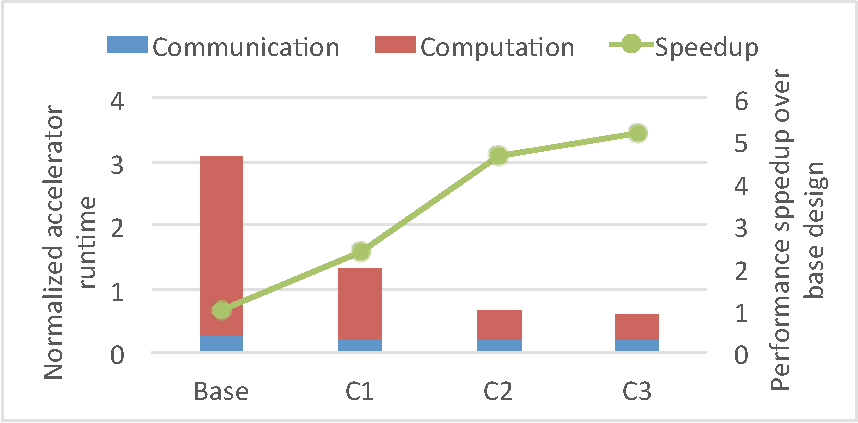
\includegraphics[width=0.47\linewidth]{qd_customization_ex}
\label{fig:qd_customization_ex}
}
\hfill
\subfigure[Resource Consumptions]{
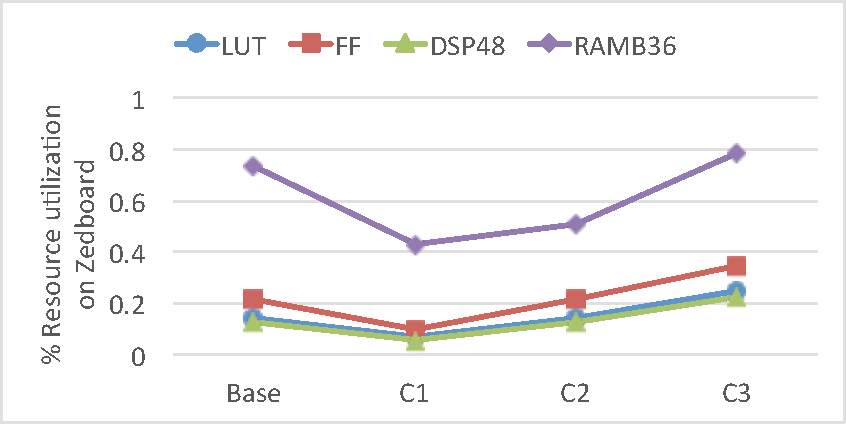
\includegraphics[width=0.47\linewidth]{qd_customization_resource}
\label{fig:qd_customization_resource}
}
\newline
\subfigure[Overlay configuration]{
\begin{minipage}{0.9\linewidth}
\centering
\footnotesize
\begin{tabular}{ccccc}
\toprule
&base&C1&C2&C3\\
\midrule
Loop unrolling factor&10$\times$50&50$\times$50&50$\times$50&50$\times$50\\
Grouping factor&100$\times$50&2500$\times$50&1250$\times$50&5000$\times$50\\
SCGRA size&3$\times$3&2$\times$2&3$\times$3&4$\times$4\\
Inst Mem Depth&4k&4k&2k&1k\\
IO Buffer Depth&1k&4k&2k&8k\\
\bottomrule
\end{tabular}
\end{minipage}
}
\caption{Effect of overlay customization on performance and resource consumption.  Example here shows the result of an FIR filter using QuickDough with 3 different overlay configurations over a base design.}
\label{fig:qd_customization_fir}
\end{figure}

A few interesting observations can be made from the figures.  In terms of performance, comparing to the sub-optimal baseline configuration, the best configuration (\textsc{c3}) results in more than 5 times improvement in performance.
Furthermore, comparing the baseline and \textsc{c2} that feature the same array size ($3\times 3$), $4.7\times$ improvement in performance can be obtained by optimizing the unrolling and grouping factor in combination with the on-chip memory configuration.
Interestingly, looking at the resource consumptions, \textsc{c2} in fact consumes $31\%$ less on-chip memory and the same resource otherwise as the baseline.

\subsection{Summary}
Using QuickDough as a case study, we have illustrated how the use of an FPGA overlay has enabled a very different experience for software programmers when designing hardware-software systems.
The 2-layer approach to hardware design allows for a very rapid design experience that sharply contrasts the lengthy low-level hardware tool flow.
Furthermore, the softness of the overlay provides opportunity for further customization and optimization as the development effort progresses.
Together, it creates for novice users a ``software-like'' way to designing complex accelerator systems while maintaining considerable overall acceleration performance promised by FPGAs.



%%
%%
%%
%%



%%%%%%%%%%%%%%%%%%%%%%%%%%%%%%%%%%%%%%%%%%%%%%%%%%%%%%%%%%%%%%%%%%
% END   QUICKDOUGH.TEX
%%%%%%%%%%%%%%%%%%%%%%%%%%%%%%%%%%%%%%%%%%%%%%%%%%%%%%%%%%%%%%%%%%

\section{Research Challenges \& Opportunities}
%While the early results of using FPGA overlay are encouraging, there remain many challenges that must be overcome before its full potential can be unleashed.
%
%While the potential of FPGA overlay is plentiful, there remain many challenges lying ahead that warrant future research.
In particular, for FPGA overlays to be useful, future research must be able to address two important challenges: reduce overhead and enhance customization.

\subsubsection{Reducing Overhead}
By introducing an additional architectural layer between a user application and the physical fabric, an FPGA overlay inevitably incurs additional performance and area overhead to the system.
It is especially important when the FPGA is used as an accelerator in a processor-based system. 
If the overhead is so large that the FPGA is no longer offering any significant performance enhancement, then software programmers will have little incentive to devote effort into using them.

From a hardware implementation's point of view, the additional layer must also incur additional area overhead.
Such overhead usually manifests as additional usage of configurable fabric and on-chip memory.
In some cases where spare resources are available, the effect of such area overhead may not be apparent.
In fact, as illustrated earlier, researchers have deduced ways to make sure of such spare resources for debugging purposes \cite{Hung:2013:TSO:2435264.2435272}.
However, in other cases where the area of FPGA overlay results in a reduction of resources available to implement a user's design, then it is likely that this area overhead will translate into performance overhead.
On a circuit level, such area overhead may also manifest as additional delays impose on the critical path, resulting in overall performance loss.
Therefore in short, area overhead, if not well controlled, may easily translate into performance overhead.

Luckily, as mentioned in some early works, despite such overhead, the use of an overlay may still be worthwhile from a performance perspective.  For example in \cite{capalijia2013pipelined}, Capalija and Abdelrahman has demonstrated that by taking advantage of the regularity of its overlay and with the help of detailed floor planning, they were able to control the overhead while maintaining reasonable throughput performance when compared to a simple push-button synthesis flow.
The very use of overlay allows amortization of the optimization effort in the long run as the overlay structure may be reused many times.

\subsubsection{Enhancing Customization}
Another major challenge faced by overlay designers is the very notion of using FPGA overlay in the first place:
``If by overlaying a different architecture over an FPGA may provide all sort of nice properties, then why not implement the overlay architecture directly on silicon to enjoy all the benefits instead?''
For example, if a GPU overlay provides good performance and good programmability, then maybe the design should be implemented on an actual GPU instead of a GPU overlaying on top of an FPGA.

Indeed, if the so called ``overlay'' in question is simply a fixed reimplementation of another architecture on an FPGA, then the only incentive to so are probably to provide compatibility through virtualization, or simply to save cost on silicon implementation.
In the latter case, this intermediate architecture may hardly be called an ``overlay'' any more.

However, the true power of FPGA overlays is that they can be adapted to the application through \emph{customization}.
As a virtual architecture, many aspects of an overlay architecture can be customized to the target application to improve power-performance.
In \cite{Lebedev2010}, for example, the computational core in the multi-core overlay may be customized to the specific targeted application.
By customizing the core to their targeted application, almost 10x improvement in the overlay performance can be observed, bring the overlay performance to be within factor of 3 of the reference custom FPGA design.
In \cite{Lin:2012:EDC:2460216.2460227}, the direct connection topology among the process elements in coarse-grained reconfigurable array overlay was customized against the input application. 
When compared to the best predefined topology, the application-specific interconnect provides up to 28\% improvement in resulting energy-delay product.

The improved results should come at no surprise: the extreme case of an overlay customization is simply a full-custom design of the application on the target FPGA, which is supposed to have the best possible performance if designed correctly.
What is challenging is therefore to ability to fine-tune the tradeoff among design productivity, virtualization and performance of the resulting system.
In other word, the research question to ask in the future should therefore be: ``How to improve performance of an overlaying system through customization without significantly sacrificing the benefits of using an overlay?''
The answer to this question is going to open up a wide field of exciting research in FPGA-based reconfigurable systems.

\subsubsection{Closing Thoughts}
FPGA overlay is without doubt going to be an important part of future FPGA-based reconfigurable systems.
The potential is plentiful and we anticipate that overlaying technology will benefit all aspects of future reconfigurable systems, especially on the important aspect of design productivity.
With silicon technologies continue to evolve, the amount of available on-chip configurable resource is going to increase.
The abundance of high-performance configurable resources on FPGA will enable a new generation of systems that relies heavily on advanced overlay architectures for virtualization and to improve design productivity. 


While the early results of using FPGA overlay are encouraging, there remain many challenges that must be overcome before its full potential can be unleashed.
%
%While the potential of FPGA overlay is plentiful, there remain many challenges lying ahead that warrant future research.
In particular, for FPGA overlays to be useful, future research must be able to address two important challenges: reduce overhead and enhance customization.

\subsection{Reducing Overhead}
By introducing an additional architectural layer between a user application and the physical fabric, an FPGA overlay inevitably incurs additional performance and area overhead to the system.
It is especially important when the FPGA is used as an accelerator in a processor-based system. 
If the overhead is so large that the FPGA is no longer offering any significant performance enhancement, then software programmers will have little incentive to devote effort into using them.

From a hardware implementation's point of view, the additional layer must also incur additional area overhead.
Such overhead usually manifests as additional usage of configurable fabric and on-chip memory.
In some cases where spare resources are available, the effect of such area overhead may not be apparent.
In fact, as illustrated earlier, researchers have deduced ways to make sure of such spare resources for debugging purposes \cite{Hung:2013:TSO:2435264.2435272}.
However, in other cases where the area of FPGA overlay results in a reduction of resources available to implement a user's design, then it is likely that this area overhead will translate into performance overhead.
On a circuit level, such area overhead may also manifest as additional delays impose on the critical path, resulting in overall performance loss.
Therefore in short, area overhead, if not well controlled, may easily translate into performance overhead.

Luckily, as mentioned in some early works, despite such overhead, the use of an overlay may still be worthwhile from a performance perspective.  For example in \cite{capalijia2013pipelined}, Capalija and Abdelrahman has demonstrated that by taking advantage of the regularity of its overlay and with the help of detailed floor planning, they were able to control the overhead while maintaining reasonable throughput performance when compared to a simple push-button synthesis flow.
The very use of overlay allows amortization of the optimization effort in the long run as the overlay structure may be reused many times.

\subsection{Enhancing Customization}
Another major challenge faced by overlay designers is the very notion of using FPGA overlay in the first place:
``If by overlaying a different architecture over an FPGA may provide all sort of nice properties, then why not implement the overlay architecture directly on silicon to enjoy all the benefits instead?''
For example, if a GPU overlay provides good performance and good programmability, then maybe the design should be implemented on an actual GPU instead of a GPU overlaying on top of an FPGA.

Indeed, if the so called ``overlay'' in question is simply a fixed reimplementation of another architecture on an FPGA, then the only incentive to so are probably to provide compatibility through virtualization, or simply to save cost on silicon implementation.
In the latter case, this intermediate architecture may hardly be called an ``overlay'' any more.

However, the true power of FPGA overlays is that they can be adapted to the application through \emph{customization}.
As a virtual architecture, many aspects of an overlay architecture can be customized to the target application to improve power-performance.
In \cite{Lebedev2010}, for example, the computational core in the multi-core overlay may be customized to the specific targeted application.
By customizing the core to their targeted application, almost 10x improvement in the overlay performance can be observed, bring the overlay performance to be within factor of 3 of the reference custom FPGA design.
In \cite{Lin:2012:EDC:2460216.2460227}, the direct connection topology among the process elements in coarse-grained reconfigurable array overlay was customized against the input application. 
When compared to the best predefined topology, the application-specific interconnect provides up to 28\% improvement in resulting energy-delay product.

The improved results should come at no surprise: the extreme case of an overlay customization is simply a full-custom design of the application on the target FPGA, which is supposed to have the best possible performance if designed correctly.
What is challenging is therefore to ability to fine-tune the tradeoff among design productivity, virtualization and performance of the resulting system.
In other word, the research question to ask in the future should therefore be: ``How to improve performance of an overlaying system through customization without significantly sacrificing the benefits of using an overlay?''
The answer to this question is going to open up a wide field of exciting research in FPGA-based reconfigurable systems.

\subsection{Closing Thoughts}
FPGA overlay is without doubt going to be an important part of future FPGA-based reconfigurable systems.
The potential is plentiful and we anticipate that overlaying technology will benefit all aspects of future reconfigurable systems, especially on the important aspect of design productivity.
With silicon technologies continue to evolve, the amount of available on-chip configurable resource is going to increase.
The abundance of high-performance configurable resources on FPGA will enable a new generation of systems that relies heavily on advanced overlay architectures for virtualization and to improve design productivity. 



%\dominitoc% Initialization
%\tableofcontents

%\chapter[FPGA Overlay]{Coarse-Grained Architectures and Overlays}
%\minitoc

%\begin{center}
\Large Outline
\end{center}

\begin{raggedleft}
\footnotesize

\begin{itemize}[nosep]
\item Motivation
\begin{itemize}[nosep]
\item Difference in hardware and software design experience
\item Many features trivially expected by modern software designers are not available in hardware -- high design productivity, fast debug cycles, relocatable code, portability, virtualization, etc.
\item  Overlay provides many of such features
\end{itemize} % 1st level
\item FPGA Overlays

\begin{itemize}[nosep] % 2nd level

\item
Definition of overlay
\begin{itemize}[nosep]
\item Definition: A virtual reconfigurable architecture that overlays on top of the physical FPGA configurable fabric.
\end{itemize}

\item
Overlay vs Custom Design vs CGRA
\begin{itemize}[nosep]
\item  Although very similar, overlay $\ne$ custom design
\item Overlays are designed to be somewhat general purpose (or at least compatible with a domain of applications)
\item  Overlay $\ne$ plain, hard, CGRA
\item The use of CGRA is a mean to achieve other goals in the overlay.
\item  The CGRA is ``soft'' by design
\end{itemize}

\item
Benefits of Overlays
\begin{itemize}[nosep]
\item Virtualization
\begin{itemize}
\item Portability
\item Security
\item Compatibility
\end{itemize}
\item Design productivity
\begin{itemize}
\item Compilation time
\item Debugging facilities
\end{itemize}
\item HW/SW Separation of Concerns 
\begin{itemize}
\item SW: map application to overlay, which is more software friendly
\item HW: map overlay to physical hardware
\end{itemize}

\end{itemize}

\item
Short Survey of existing Overlay Designs
\begin{itemize}[nosep]
\item Virtual FPGAs
%\item Hard macro/modular design methodologies
\item CGRAs
\item Multi-core/MPPA/Other processor arrays
\item GPU / OpenCL overlay
\item etc
\end{itemize}
(Questions: maybe we want to categorize overlays according to the intended uses (e.g. security, portability, etc)
(Another way to categorize them will be by their different architecture)
(The work presented at OLAF can be a good starting point on a survey of existing overlay projects.)
\end{itemize} %end 2nd level

\item
Case Studies
Here we show various examples of overlays as “case studies”.

\begin{itemize}[nosep]
\item QuickDough
\item Malibu? Zuma?
\end{itemize}

\item
State-of-the-art and availability/usability for software engineers
\begin{itemize}[nosep]
\item (I don’t think there is any commercially available overlay offer.  Software compatibility layers may be available in some way.
\item e.g. Think of VPR and the “virtual” target FPGA. It can be a compatibility target for different FPGA vendors if needed.)
\item Tools for Overlays?
\end{itemize}
\end{itemize}

\end{raggedleft}
 % delete me later
%\section*{Hayden's Draft}
%=== Hayden's Draft ===

Hardware compilation experience:
slow (minutes vs days for the largest designs)
portable across devices within family only when timing allows
rarely portable across vendor (different memory, different FIFO timing, etc)
Not even portable to different accelerator systems with the same FPGA devices due to different connections.


Overall idea and benefits of using overlays on FPGAs
Definition:


A virtual reconfigurable architecture that overlays on top of the physical FPGA configurable fabric.
	

It is ``virtual'', because the overlay architecture may not necessarily be implemented physically in the final design.  It is ``reconfigurable'', because the overlay has to support customization for more than one applications.


Unfortunately, and also fortunately, because of the flexibility of FPGAs, the exact definition of an overlay can sometimes be difficult to precisely define.  If you implement a Commodore 64 system on an FPGA so you can play your favorite 8-bit games on FPGA, are you implementing a game system or is it already a ``overlay’’ in the form of a CPU system?
What if you now upgrade this classic system to become a massively multi-core processor system for parallel execution of game code?  Would that make it more of an overlay than the simple soft CPU core?


In the straightest sense according to the above definition, a simple soft CPU core implemented on FPGA can be called an overlay -- it is virtual as you can implement the same CPU differently on different FPGAs, providing portability and compatibility.  At the same time, it is also reconfigurable, as you can obviously execute a broad range of applications on this CPU by programming it with different software.


In practice, however, the concept of an FPGA overlay is a lot more far reaching than a simple soft CPU core.  It encompass all sort of compute architectures one can imagine, with many of them designed specifically for the purpose of serving as an overlay.  These overlay are specifically designed for the goal at hand: for virtualization, for efficiency, for power-performance tradeoff, for design productivity.  They are also specially designed for use in FPGA with low overhead.


Sometimes such overlay may not even literally exist in the final physical design.  For example a word-based FPGA may exist only in the form of design constraint or is embedded in the design language, while its architectural features may not necessarily be implemented on the FPGA (e.g. any unused word-mux defined in the architecture doesn't need to be implemented.)  It is as opposed to constructing this word-based FPGA physically on silicon.


== Random Draft ==


What are not overlays?


A custom architecture for a specific problem.  For example, you have designed a new architecture for performing FFT on FPGAs, say it is FFTA, that is very efficient for your own application A.  It works well on your own application, but it may or may not be directly reusable in another application.  I may be reused as a hard IP block, or even a retargetable library component, but it can hardly be called an overlay.  But the line starts to blur if this FFT block is indeed highly parameterizable and is implemented as an intermediate virtual layer in certain design framework.


Similarly, an array of flexible processing element connected in a mesh 


===
RANDOM DRAFT


--
In many ways, an overlay architecture is similar to an overlay network -- An overlay architecture exists be fulfill certain technological requirements.  In the case of an overlay network, it may be designed so as to provide better quality of service, or to provide better security, or even better management domain.  Similarly, researchers have developed a wide range of overlay architectures to improve the FPGA design experience.  


--


The easiest way to understand what an FPGA overlay is, is to consider building a \emph{virtual} FPGA (\textsc{vf}) using the configurable fabric of a physical FPGA (\textsc{pf}).  By doing so, you now have an FPGA overlay architecture in the form of \textsc{vf} overlaying on top of \textsc{pf}.  We say that \textsc{vf} is essentially ``virtual’’ because architectural features of \textsc{vf}, such as its muxes or an I/O blocks, may not necessarily be presence in a \textsc{pf}.  Yet, if the overlay is constructed correctly, any design that was originally targetting \textsc{vf} may now execute unmodified on top of \textsc{pf} without knowing the details of \textsc{pf}.


Now why would you want to overlay \textsc{vf} on top of \textsc{pf}?  The list of reasons is long but essentially similar to the reason why overlay network or architecture virtualization are performed: security, isolation, compatibility, virtualization, etc.  With this, you can imagine running design originally compiled for FPGA from vendor A to run on FPGAs from vendor B, or to allow legacy design to run on newer generations of FPGAs from the same vendor.


The power of FPGA overlay becomes even more apparent when you consider the wide varieties of compute architectures that can be constructed as overlays.  In fact, over the past decade, a wide range of coarse grained reconfigurable architectures have been explored to serve as overlays \cite{}, and has arguably become the de facto definition of many recent overlay designs \cite{}.


Coarse-Grained Architecture
The basic idea of a coarse-grained architecture is to reduce the configuration granularity of an FPGA from its physical fine-grained configurable fabric (LUT, routing) to one with coarser reconfiguration granularity.  The fundamental goal is thus to improve power-performance and design productivity of the resulting fabric by trading off design flexibility.


This notion of reduced granularity works very well in overlay design as a way to improve design productivity.  Coarse-grained architectures improve a designer’s productivity in two fundamental ways.  First, by constraining the flexibility of an FPGA, a coarse-grained architecture reduces the design space significantly, which reduces implementation tool flow run time considerably \cite{quickdough,hmflow}. In addition, many coarse-grained architectures implement a compute models that are more familiar to software designers, considerably lowering the barrier-to-entry to employ such designs.  For instance, many recent overlays are implemented as coarse-grained reconfigurable arrays (CGRAs), where computation is carried out by a connected array of processing elements (PEs) instead of relying on user-generated random logic implemented on the FPGA.  To many software programmer, programming a parallel processor array, while a daunting task in its own right, is still a lot easier than to implement designs on the native FPGA configurable fabric.


--


Different CGRA architectures differ considerably.  At one end of the spectrum, researchers have proposed various configurable coarse grained hardware.  The blocks are in the level of arithmetic units.  Users configure the their design by specifying the static route between these blocks.


On the other end of the spectrum, there are multi-core processors connected with an elaborated on-chip packet switching network, essentially forming a system-on-chip.


---


Imagine, for example, to construct a previous generation FPGA using a newer generation FPGA.  By imposing this hypothetical overlay architecture of another FPGA, user can now experience something new:

\begin{itemize}
\item isolation
\item backward compatibility
\item virtualization
\end{itemize}

These are very similar benefits to that provided through virtualization of conventional CPU-based system.  But just like CPU virtualization, it comes at a price:

\begin{itemize}
\item speed
\item cost
\item power
\end{itemize}


=== RANDOM DRAFT ===


---- From Old Paper ---
To improve the speed of low-level implementation tools, researchers have explored various approaches over the past decades.
Inspired by application specific integrated circuit (ASIC) design flows, researchers and vendors have developed modular design flow and explored the use of pre-compiled hard macros \cite{lavin2010using,lavin2011} as implementation library.
In addition, researchers have also exploited the use of dynamic partial reconfiguration capabilities in FPGAs \cite{Frangieh2010} as a way to improve productivity.
In recent years, there has been an increased interest in applying the concept of \emph{overlay architectures} as a way to address this productivity challenge.  




An overlay architecture is a virtual intermediate architecture that is overlaid on top of the physical configurable fabric of an FPGA.  They are employed during the FPGA application implementation process for purposes such as to improve portability, security, and also productivity.
%Depending on the design goal, overlays have manifested in various forms, including HDL models, pre-synthesized or pre-implemented coarse-grained circuits, or even arrays of processing elements with various granularity.


One of the most familiar categories of overlay consists of virtual FPGAs \cite{zuma2013carl,Grant2011Malibu,Coole2010Intermediate,Koch2013CI}. They are built either virtually or physically on top of off-the-shelf FPGA devices and typically feature coarser configuration granularity than the physical device.
Similar to virtual machines running on a typical computer, such virtual FPGA provides an additional layer that improves application portability and security.
Furthermore, because of the coarser-grained configurable fabric, implementing designs on such overlay is relatively easier than on a fine-grained device.
However, the additional layer imposes restrictions on the underlying fabrics' capability and usually results in moderate hardware overhead and timing degradation.


Another category of overlay architecture commonly employed is in the form of coarse-grained reconfigurable arrays (CGRAs).
The use of CGRAs provides unique advantages of compromising hardware implementation and performance especially for compute intensive applications as demonstrated by numerous ASIC CGRAs \cite{tessier2001reconfigurable} \cite{compton2002reconfigurable}.
Indeed, CGRAs on FPGA and ASIC have many similarities in terms of the scheduling algorithm and array structure.
However, they have quite different trade-offs in terms of configuration flexibility, overhead and performance.
In a nutshell, CGRAs on ASIC emphasize more on configuration capability to cover more applications, while FPGAs' inherent programmability greatly alleviates the concern.
Instead, CGRAs on FPGA may take advantage of the configurability of the underlying fabric to allow more intensive customization tailored to the target application.


The authors in \cite{kissler2006dynamically} developed WPPA (weakly programmable processor array), a VLIW architecture based parameterizable CGRA overlay. It featured an interconnection wrapper unit for each processing element (PE) that could be used for dynamic CGRAs topology customization. Unfortunately, programming and compilation on WPPA were not presented. The authors in \cite{ferreira2011fpga} proposed a heterogeneous CGRA overlay with a global multi-stage interconnection on FPGA. Compiling applications onto the overlay took only milliseconds for smaller DFGs. However, the global multi-stage interconnection required multiple stages for communication between each pair of PEs and resulted in either low implementation frequency or large communication latency in terms of cycles. In addition, there was no intermediate storage except the pipeline registers in the CGRA and it limited the performance of the operation scheduling.
In \cite{shukla2006quku}, a customized CGRA overlay called QUKU was developed for DSP algorithms. It had two-level configuration capability, while the low-speed configuration was used for operator reuse within an application and high-speed reconfiguration was used for optimization between different applications. Nevertheless, the hardware infrastructure was consist of simple operation elements which can only be adapted to a few specified DSP algorithms.
The authors in \cite{capalijia2013pipelined} built a more generic high speed mesh CGRA overlay using the elastic pipeline technique to achieve the maximum throughput. It adopted a data-driven execution flow and was suitable for smaller pipelined DFG execution, while it would be difficult to handle applications with random IO access.


In general, previous CGRA overlays have demonstrated the promising performance acceleration capability for compute intensive applications. They typically take DFG as design entry and focus on hardware infrastructure design as well as corresponding mapping and scheduling. However, they are still lack of consideration on proper loop unrolling for DFG generation, on-chip buffering, the communication with host and even end-to-end performance which are essential for FPGA accelerator design especially from a HW/SW co-design engineer's perspective.




Finally, a third category of overlay features soft-processor-like architectures with high degree of control and data parallelism suitable for FPGA accelerations.  For example, in the work of MARC \cite{Lebedev2010}, a many-core overlay with customizable data path was proposed.  Similarly, a GPU-like overlay was proposed in \cite{Jeffrey2011potential}.

 % draft from Hayden
%\section*{Guy's Draft}
%\input{guy} % draft from Guy


% \noindent
% \begin{minipage}{\linewidth}
% \centering
% \fbox{\Huge\bf Start of Real Content}
% \end{minipage}

%%%% Real Content %%%%
%\section{Motivation}
% \section{Motivation} \label{sec:motivation}
Clock frequency determines the accelerator operation speed 
and directly affects the performance. Accordingly, it also has influence on the 
neural network runtime and energy efficiency. In this section, we take 
an open-sourced CNN accelerator named PipeCNN \cite{pipecnn_2} as an example and analyze its 
influence on the neural network performance and energy efficiency.

The accelerator is implemented on KCU1500 and attached to a desktop computer with 
Intel i7-6700@3.40GHz. The basic convolution structure is shown in Fig \ref{fig:cnn-arch}. The largest computing 
array that can be accommodated by the FPGA device consists of 16 dot production units. 
Each dot production unit allows parallel processing of two 8-data vectors.
The accelerator consumes over 11\% LUT of the FPGA device. The optimized clock frequency 
according to the SDAccel compilation is 200 MHz. 

\begin{figure}
	\center{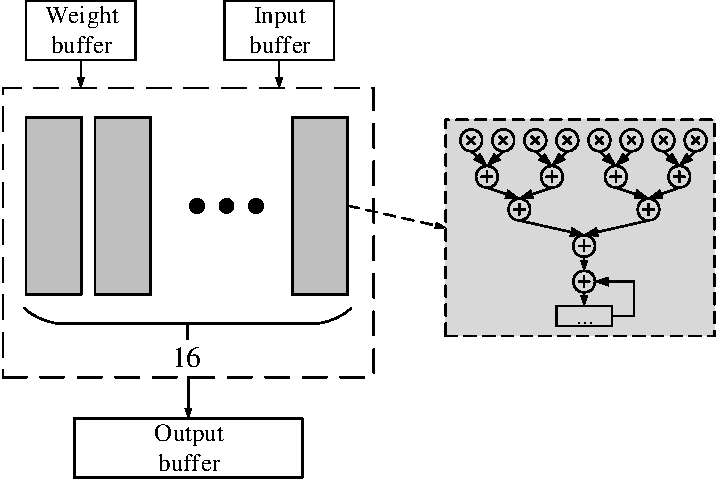
\includegraphics[width=0.75\linewidth]{accelerator}}
    \caption{Baseline CNN accelerator architecture.}
\label{fig:cnn-arch}
\vspace{-1em}
\end{figure}


In order to evaluate the influence of clock 
frequency, we further set the clock to 50 MHz, 100 MHz, and 150 MHz respectively.
A set of neural networks including LeNet, AlexNet, VGG-16 and VGG-19 are used as the benchmark.
Normalized performance the neural network benchmark executed on the accelerators are 
shown in Fig \ref{fig:computing-bound}. It can be found that the 
overall performance of the neural network benchmark
almost increases proportional to the clock frequency. For the larger neural networks, 
the processing remains the computing bound and high frequency design is highly demanded.

\begin{figure}
	\center{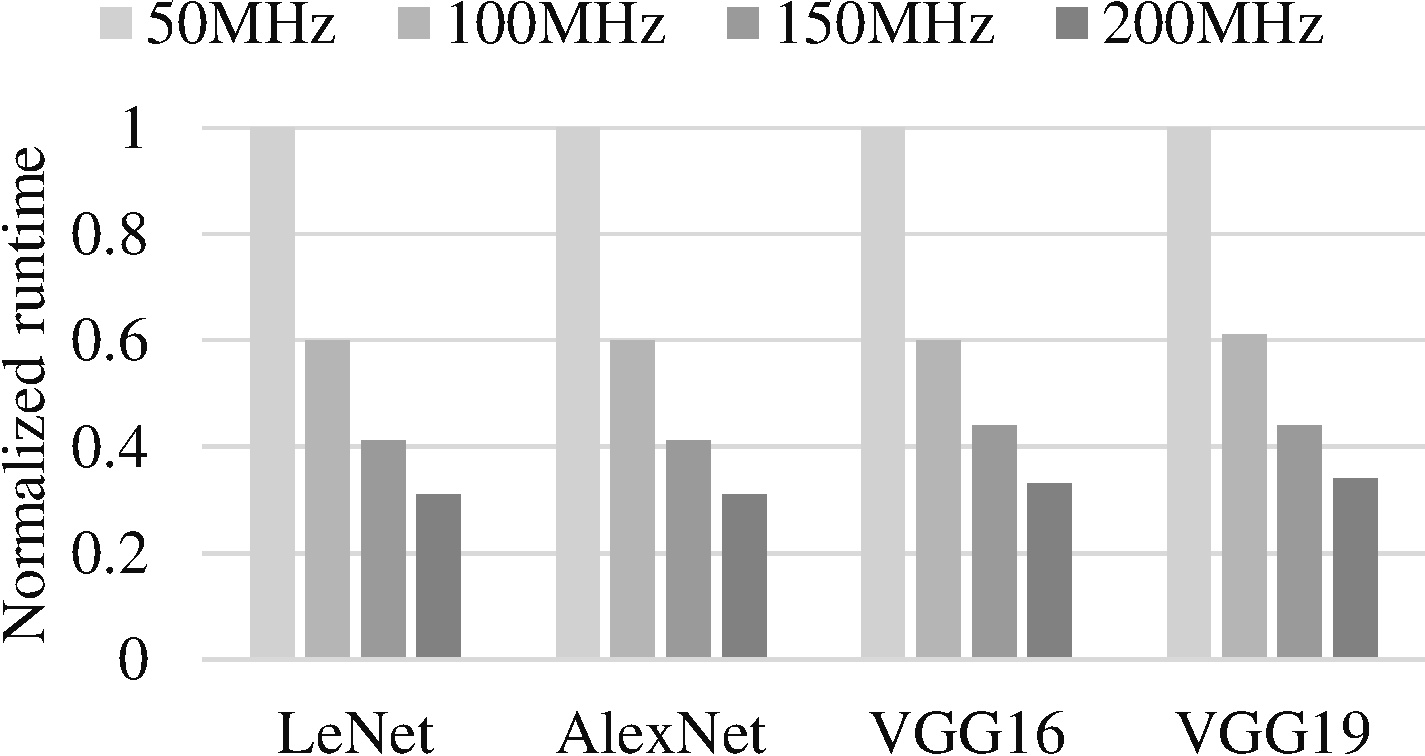
\includegraphics[width=0.75\linewidth]{relative_time}}
    \caption{Normalized performance of neural networks executed on CNN accelerators with different clock frequency.}
\label{fig:computing-bound}
\vspace{-1em}
\end{figure}

In addition, we also obtain the power consumption from SDAccel report. 
The power estimation setup assumes xxxx. Given the power consumption and the performance, 
we calcualted the energy delay product which can be used as an energy efficiency metric.
The energy efficiency is presented in Fig \ref{fig:edp}.
\begin{figure}
	\center{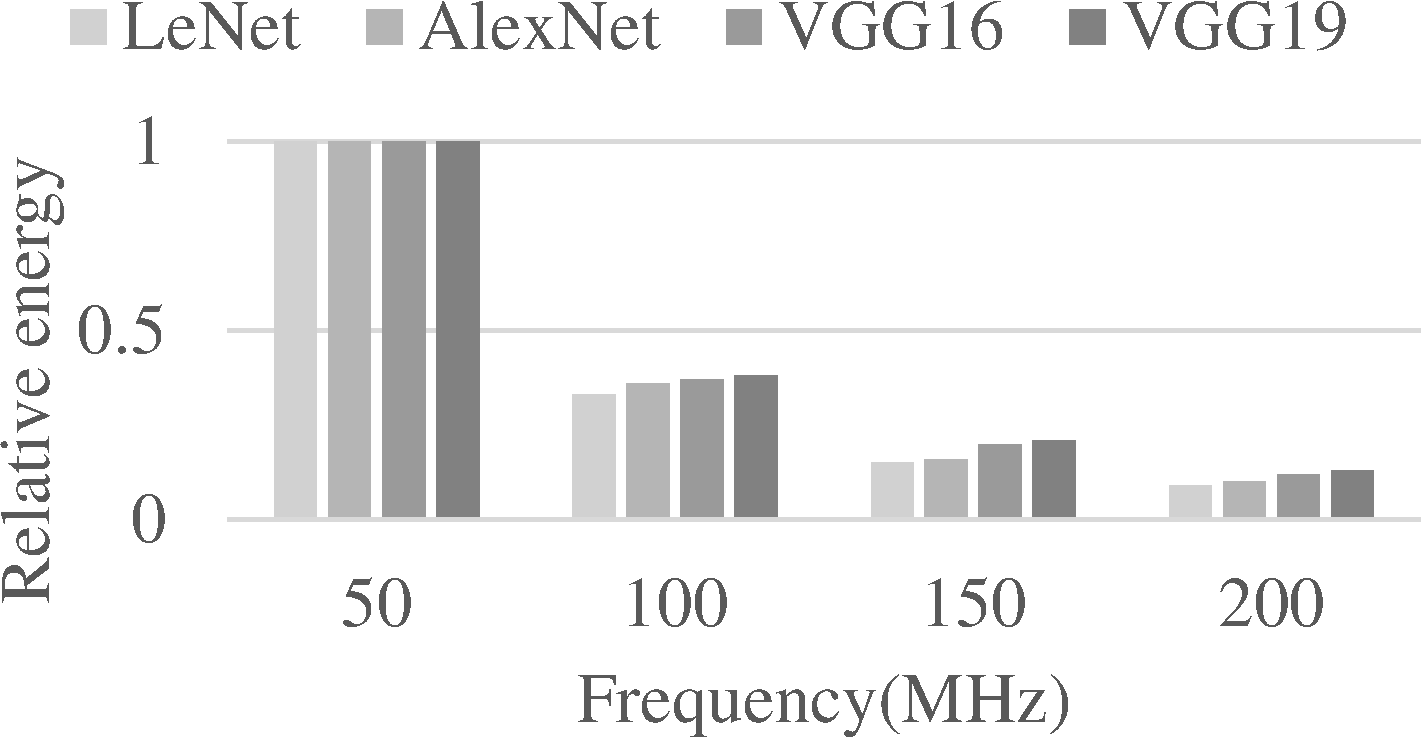
\includegraphics[width=0.75\linewidth]{relative_energy}}
    \caption{Normalized energy-delay product of neural networks executed on CNN accelerators with different clock frequency.}
\label{fig:edp}
\vspace{-1em}
\end{figure}

According to the above experiments, it can be conclcuded that higher clock frequency 
can be beneficial to both the neural network performance and energy efficiency. The 
potential performance and energy efficiency improvement indicates that it is 
worthwhile to boosting the clock of FPGA based CNN accelerators with some minor 
overhead. Detailed overclocking on CNN accelerators will be investigated in 
detail in the rest part of this paper. 

% \section{Overview}
% The concept of overlaying a virtual architecture over a physical system is not entirely new -- in networking, for example, virtual overlay networks are routinely constructed on top of the physical infrastructure in modern systems.
On the other hand, the concept of overlaying a virtual architecture over a physical FPGA is only recently gaining traction among researchers, but is already generating a lot of excitements because of their potentials.


% \begin{center}
% \fbox{\begin{minipage}{\linewidth}
% A virtual reconfigurable architecture that overlays on top of the physical FPGA configurable fabric.
% \end{minipage}}
% \end{center}

So what is an FPGA overlay exactly?
Interestingly, because of the unique nature of FPGAs as a flexible configurable hardware, drawing up a precise definition for an FPGA overlay may not be as straightforward as it may seem. 
In this chapter, we will use the following definition as a starting point.

\begin{quote}
An FPGA overlay is a virtual reconfigurable architecture that overlays on top of the physical FPGA configurable fabric.
\end{quote}

From this definition, we can see that an FPGA overlay is a machine architecture that is able to carry out certain computation.  Furthermore, this architecture is \emph{virtual} because the overlay may not necessarily be implemented physically in the final design.  Finally, it is \emph{reconfigurable} because the overlay must be able to support customization or be reprogrammed to support more than one applications.

In other words, an FPGA overlay is a virtual layer of architecture that conceptually locates between the user application and the underlying physical FPGA similar to that shown in \figref{fig:overlay_overview}.
With this additional layer, user applications will no longer be implemented onto the physical FPGA directly.
Instead, the application will be targeted toward the overlay architecture regardless of what the physical FPGA may be.
A separate step will subsequently translate this overlay architecture, together with the application that runs on it, on to the physical FPGA.

\begin{figure}
\centering
\includegraphics[width=0.5\linewidth]{overlay_overview}
\caption{Using an overlay to form a 2-layer approach to FPGA application development.  Overlay may be designed as a virtual FPGA, or it may implement an entirely different compute architecture such as a coarse-grained reconfigurable array (CGRA), vector processor, multi-core process, or even an GPU.}
\label{fig:overlay_overview}
\end{figure}

The easiest way to understand how an FPGA overlay operates in practice, is to consider building a \emph{virtual} FPGA (\textsc{va}) using the configurable fabric of a physical FPGA (\textsc{pa}).  By doing so, you now have an FPGA overlay architecture in the form of \textsc{va} overlaying on top of \textsc{pa}.  We say that \textsc{va} is essentially ``virtual'' because architectural features of \textsc{va} such as its muxes or I/O blocks may not necessarily be present in \textsc{pa}.  Yet, if the overlay is constructed correctly, any design that was originally targeting \textsc{va} may now execute unmodified on \textsc{pa} without knowing its details.

However, the power of employing FPGA overlay is not limited to making virtual FPGAs only.
On the contrary, taking advantage of FPGA's general-purpose configurable fabric, many researchers have demonstrated the benefits of overlays that implement entirely different computing architectures such as 
multi-core processor system, coarse-grained reconfigurable arrays (CGRAs), or even general-purpose graphic processing units (GPUs).

Now, using a multi-core processor overlay as an example, it should be apparent how overlays are able to improve a software programmer's design productivity.
Instead of working with unfamiliar hardware-centric tools and design methodologies, software programmers are now possible to utilize FPGAs as accelerators simply by writing programs that target a familiar architecture.
In general, one benefit of using FPGA overlay is that it is able to bridge between the often software-inclined user and the low-level FPGA hardware fabric.

Of course, if an application can be readily accelerated on a multi-core processor overlay implemented using FPGAs, then it is understandably begging the question: why not simply run the design on an actual high-performance multi-core processor instead?
The answer to this question, indeed, is the key challenge that will guide the future research on overlay designs --- While an overlay offers many desirable features to software programmable such as improved design productivity, the additional layer on top of the physical FPGA inevitably introduces additional performance penalty to the system.
A good overlay design must therefore ensure that despite the performance penalty introduced, the overall acceleration offered by FPGA must remain competitive for the accelerator system to be worthwhile.
Furthermore, it must provided added value beyond a solution with a fixed general-purpose architecture.
One such added value is the ability to customize the overlay for the particular application or group of applications concerned for sake of performance or power-efficiency.



\iffalse

Unfortunately, and also fortunately, because of the flexibility of FPGAs, the exact definition of an overlay can sometimes be difficult to precisely define.  If you implement a Commodore 64 system on an FPGA so you can play your favorite 8-bit games on FPGA, are you implementing a game system or is it already a ``overlay'' in the form of a CPU system?
What if you now upgrade this classic system to become a massively multi-core processor system for parallel execution of game code?  Would that make it more of an overlay than the simple soft CPU core?


In the straightest sense according to the above definition, a simple soft CPU core implemented on an FPGA can be regarded as an overlay -- it is virtual as you can implement the same CPU differently on different FPGAs, providing portability and compatibility.  At the same time, it is also reconfigurable, as you can obviously execute a broad range of applications on this CPU by programming it with different software.


In practice, however, the concept of an FPGA overlay is a lot far reaching than a simple soft CPU core.  It encompasses all sorts of compute architectures one can imagine, with many of them designed specifically for the purpose of serving as an overlay.  These overlays are specifically designed for the goal at hand: for virtualization, for efficiency, for power-performance tradeoff, for design productivity, etc.  They are also specially designed for use in FPGA with low overhead.

\fi

%Sometimes such overlay may not even literally exist in the final physical design.  For example a word-based FPGA may exist only in the form of design constraint or is embedded in the design language, while its architectural features may not necessarily be implemented on the FPGA (e.g. any unused word-mux defined in the architecture doesn't need to be implemented.)  It is as opposed to constructing this word-based FPGA physically on silicon.

\subsection{Coarse-Grained Architectures}
In most cases, FPGA overlays are essentially coarse-grained architectures that are built on top of the physical fine-grained configurable fabric.
As their names suggest, the basic idea of a coarse-grained architecture is to reduce the configuration granularity of an FPGA from its physical fine-grained configurable fabric such as LUTs to one with coarser reconfiguration granularity.
In some cases, such coarse-grained blocks may refer simply to arithmetic blocks of moderate sizes such as adders, multipliers, or digital signal processing blocks of some sort.
In other cases, such coarse-grained blocks may refer to very complex microprocessors connected with sophisticated network-on-chip.
Regardless of the implementation, the central goal of any coarse-grained architecture remains the same: to improve power-performance of the system by trading off design flexibility.

%From the perspective of overlay design, coarse-grained architectures are very attractive.
%Not only do they have clearly demonstrated power-performance advantages, they are also good candidates to serve as a design productivity improvement choice.

In addition, because of their reduced configuration flexibility, coarse-grained architectures can also enable design methodologies that are more productive than traditional hardware design flow.
In particular, coarse-grained architectures improve a designer's productivity in two important ways.
First, by constraining the flexibility of an FPGA, a coarse-grained architecture reduces the design space significantly, which has a net effect of reducing implementation tool flow run time considerably \cite{lavin2011}. 
In addition, many coarse-grained architectures implement compute models that are more familiar to software designers, considerably lowering the barrier-to-entry to employ such designs.  For instance, many recent overlays are implemented as coarse-grained reconfigurable arrays (CGRAs), where computation is carried out by a connected array of processing elements (PEs).
Instead of implementing the user application using low-level configurable logic of the FPGA, these operations are translated into computational tasks that take place in the PEs.
To many software programmers, programming a parallel processor array, while a daunting task in its own right, is arguably a lot more approachable than to implement designs on the native FPGA configurable fabric.
As such, it is not surprising that many recent overlay designs are built on top of an underlying coarse-grained reconfigurable array \cite{kissler2006dynamically,ferreira2011fpga,shukla2006quku,Lin:2012:EDC:2460216.2460227,capalijia2013pipelined,dspoverlay}.





\section{Benefits of Overlays}
As a virtualization layer that sits between a user application and the physical configurable fabric, an FPGA overlay inherits many of the benefits that software programmers have learned to expect from their CPU virtualization experience --- portability, compatibility, manageability, isolation, etc.  On top of that, employing FPGA overlays has also been demonstrated as a good way to improve a designer's productivity through improved compilation speed and better debugging support.  Along the same line, by carefully partitioning the complex hardware-software design flow around an intermediate overlay layer, it is also possible to provide separation of concerns between software and hardware engineers in the design team.
The overlay essentially acts as a bridge between the two teams, while allowing the overall system to take advantage of the FPGA resources efficiently.

\subsection{Virtualization}
Virtualization of FPGA resources has long been an active area of research since the early days of reconfigurable computing.  These pioneering works have demonstrated many of the possibilities as well as challenges associated with virtualizing hardware resources that are not designed to be time-multiplexed.  A common trend among these early works was that virtualization can be used as a mean to provide the designers and/or tools the illusion of having infinite hardware resources.  Early works by Trimberger et al~\cite{Trimberger97}, virtual wire\cite{virtualwire} and SCORE \cite{score}, for instances, gave the users the illusion of a system with unlimited FPGA resources through carefully structured hardware/CAD system.  Others have studied the problem of time-sharing of FPGA resources from an operating system's perspective as a way to provide shared accelerator resources among users/processes. \cite{Lubbers:2009:RMP:1596532.1596540,SoTECS08,Fu:2005:FCCM}.

As the concept of FPGA overlay continues to mature, the idea of virtualizing FPGAs has taken on a new focus.  As an overlay, virtualizing FPGAs allows an additional benefit of providing a compatibility and portability layer for FPGA designs.  In the work of Zuma~\cite{zuma2012}, for instance, virtual, embedded FPGAs were proposed.  By providing a virtual FPGA layer, the authors demonstrated that it is possible to execute the same netlist on multiple FPGAs from competing vendors using multiple different design tools.

\iffalse
\subsection{Improved Design Productivity}
An important benefit of using FPGA overlays is that they promise to improve designer's productivity in developing FPGA applications.
Design productivity is hard to measure, but has long been regarded as one of the key barrier-to-entry for novice users to start using FPGAs for their applications \cite{SoFpl06}.
In particular, FPGA overlays are particularly helpful in addressing two important aspects of this design productivity challenges: 
\begin{itemize}
\item Reduced compilation time
\item Application debug
\end{itemize}
\fi

\subsection{Reduced Compilation Time}
A key difference in design experience between software compilation and implementing FPGA designs rests on their drastically different run time of the involved tools.
With modern compiler technologies, software compilation has already become a straightforward, predictable, and most importantly, very rapid process.
Compiling even a relatively complex piece of software application rarely take longer than a few minutes on a reasonably fast computer.
On the other hand, implementing applications for FPGAs involves a complex labyrinth of low-level tools that are convoluted, unpredictable, and takes a long time to complete.
Compiling even the smallest design may take tens of minutes, while spending hours or even days on some of the largest designs are not unheard of.
Unfortunately, this 2 orders of magnitude difference in run time, together with the unpredictable nature\footnote{Placing and routing a design on nearly full FPGA, for example, may or may not succeed depending on the random algorithms involved.} and the often-mystical error reporting mechanisms\footnote{To see this, try to explain to a first-time software programmer why a functionally correct design in simulation may end up with an error message about timing violation on a net with an unknown name in the report.  Then, also try to explain to the programmer how to resolve that timing error.}, are all contributing to a very high barrier-to-entry that shies away most first time software programmers.
Technically, this much longer run time of the tools also significantly reduces the number of possible debug-edit-implement cycles per day, causing project delays as well as lowered productivity of the designers.

By using an overlay as intermediate compilation target, together with careful crafting of the design process, researchers have demonstrated how such lengthy hardware development process can be reduced significantly.
For example, in the work of Intermediate Fabric\cite{Coole2010Intermediate}, an intermediate coarse-grained reconfigurable fabric was introduced as an overlay.
With the overlay architecture, the average place and route times for the tested benchmark were significantly reduced by more than 500 times.

Similarly in the work of QuickDough, a coarse-grained reconfigurable array was used as overlay to accelerate compute intensive loop kernels.  Loops are scheduled to execute on the CGRA instead of compiling to the reconfigurable fabric.  As a result, when compared to manually generating custom hardware for the loops using standard hardware tools, up to 3 orders of magnitude reduction in compilation time was demonstrated.

\subsection{Improved Debugging Capabilities}
Unlike many software development frameworks where a range of debugging facilities and methodologies are readily available, tools for debugging applications that target FPGA-based systems are still in their infancy.
Traditional FPGA design methodologies rely heavily on cycle-accurate simulations for application development and debugging.
While such simulations are invaluable to understand the low-level operation of the FPGA, they are slow, tedious and provide only limited information about the run-time behavior of the design.
To monitor run-time behavior of a design, users must rely on even more complex in-system emulation facilities or even external testing hardware.
Taking advantage of FPGA overlays, researchers have demonstrated some promising results addressing the need for better debugging tools.

For instance, in a series of work by Hung and Wilton \cite{Hung:2014:VLSI,Hung:2013:TSO:2435264.2435272}, an overlay network was incorporated into FPGA design to facilitate insertion of trace buffers after a design has been placed and routed.
By carefully controlling the signal routes to utilize only unoccupied resources in the FPGA, they have demonstrated efficient ways to dynamically select and monitor signals during run time.

In other cases, since the overlay layer enables a virtual computing paradigm for the application developer that is different from the underlying FPGA, they also enable new debugging strategies that are more suitable to the designer. For instance in MARC, debugging the user-specified OpenCL applications that run on the generated multi-core architecture can follow traditional software debugging methodologies instead of relying on low level FPGA tools.
Not only can it greatly increase the abstraction level, but it can also allow a debugging strategy that matches the user's expectation.

\subsection{Separation of Hardware and Software Concerns}
With careful planning, it is also possible to take advantage of the 2-layer design approach offered by FPGA overlays as a natural division point between hardware and software development efforts.
Recall from \figref{fig:overlay_overview} that implementing designs via an FPGA overlay involves 2 steps: user applications must first be mapped to the overlay architecture, which is subsequently implemented to the physical fabric in a second step.
In many cases, the overlay architectures are designed so they can efficiently support the computational model expected by the model.
As a result, mapping of software applications to the overlay is usually more intuitive to software programmers than to map the same application to the physical FPGA fabric in one step.
On the other hand, mapping the overlay and the user application to the physical fabric involves intimate knowledge about the FPGA hardware implementation process.
This task is best left to a separate hardware team.
Consequently, one benefit of having an overlay is that the hardware team may now devote their efforts exclusively on implementing the relatively well-structured overlay on the fabric, rather than to implement many individual applications.
The hardware team can be more focused, and can perceivably create a better, highly optimized hardware design.

For example in the work of MARC\cite{lavin2011}, a multi-core processor-like architecture was used as an intermediate compilation target.
In this project, user applications are expressed as OpenCL programs.
To implement these applications, they are first compiled as an application-specific multi-core processor, which is subsequently implemented on the physical FPGA in a separate process.
With this set up, users no longer need to understand the detailed implementation of their algorithm on FPGAs.
Instead, they write essentially standard OpenCL programs, and focuses exclusively on writing the best code for the accelerated architecture assumed.
The task to map their OpenCL code into custom core on the target overlay, and to implement that overlay on the FPGA fabric, was left to a separate team.

In their case studies, the resulting application achieves about one third of the speedup when compared to fully custom designs.
Yet with the 2-layer approach using OpenCL, the design effort with MARC is significantly lower when compared to making a custom design of the same application.





% \section{Types of Overlays}
% Over the years, quite a few works on FPGA overlays have been developed.
In this section, we will take a quick walk through some of them and also look at various types of FPGA overlays that have been explored in the past decade.

\subsection{Virtual FPGAs}
To begin, one of the most easiest to understand categories of overlay are virtual FPGAs\cite{vFPGA,zuma2012,Grant2011Malibu,Coole2010Intermediate,Koch2013CI}. They are built either virtually or physically on top of off-the-shelf FPGA devices. These overlays have different configuration granularity but typically feature coarser configuration granularity than a typical FPGA device. Similar to virtual machines running on a typical computer, such virtual FPGA provides an additional layer that improves application portability and compatibility. Furthermore, because of the coarser-grained configurable fabric, implementing designs on such overlay is relatively easier than on a fine-grained device. However, the additional layer imposes restrictions on the underlying fabrics' capability and usually results in moderate hardware overhead and timing degradation.

In one of the earlier works, Lysecky et al. developed a relatively fine-grained virtual FPGA as firm cores expressed as structural VHDL \cite{vFPGA}. The virtual layer provides effective portability yet incurs relatively high performance and hardware overhead.
In \cite{Grant2011Malibu}, Grant et al. proposed a time-multiplexed virtual FPGA CAD framework MALIBU. The virtual FPGA used in MALIBU has both fine-grain and coarse-grain processing elements integrated into each logic cluster and can be used to reduce the compilation time significantly with moderate timing penalty. Around the same time, Coole and Stitt also proposed another island-style coarse-grained overlay called Intermediate Fabric \cite{Coole2010Intermediate}. It uses coarse-grained operators such as adders instead of logic clusters and routes data through 8 to 32 bit buses achieving both portability and fast compilation. Finally, Koch et al. developed a fine-grained FPGA overlay in \cite{Koch2013CI} to implement customized instructions on FPGAs from different vendors providing a portable application consisting of a program binary and an overlay configuration in a completely heterogeneous environment.

\subsection{Coarse-Grained Reconfigurable Arrays}
Another category of overlay architecture commonly employed is in the form of coarse-grained reconfigurable arrays (CGRAs) \cite{kissler2006dynamically, ferreira2011fpga, shukla2006quku, Lin:2012:EDC:2460216.2460227,capalijia2013pipelined, dspoverlay}. The use of CGRAs provides an efficient tradeoff between flexibility of software and performance of hardware especially for compute intensive applications as demonstrated by numerous earlier works \cite{tessier01reconfigurable,compton02reconfigurable}.
%Indeed, CGRAs on FPGA and ASIC have many similarities in terms of the scheduling algorithm and array structure. However, they have quite different trade-offs between flexibility and performance. In a nutshell, CGRAs on ASIC emphasize more on flexibility to cover more applications or at least a domain of applications, while FPGAs' inherent programmability greatly alleviates the concern. Instead, CGRAs on FPGA may take advantage of the configurability of the underlying fabric to allow more intensive customization tailored to the target application for better performance and lower hardware overhead.

In one of the earlier works in the area, Kissler et al. developed WPPA (weakly programmable processor array), a VLIW architecture based parameterizable CGRA overlay~\cite{kissler2006dynamically}. It featured an interconnection wrapper unit for each processing element (PE) that could be used for dynamic CGRAs topology customization. 
%Unfortunately, programming and compilation on WPPA were not presented. 
Around the same time in \cite{shukla2006quku}, a customized CGRA overlay called QUKU was developed for DSP algorithms. It had a two-level configuration capability, while the high-speed configuration was used for operator reuse within an application and low-speed reconfiguration was used for optimization between different applications. 
%Nevertheless, the hardware infrastructure was consist of simple operation elements which can only be adapted to a few specified DSP algorithms.
In \cite{ferreira2011fpga}, Ferreira et al. proposed a heterogeneous CGRA overlay with a global multi-stage interconnection on FPGA. Compiling applications onto the overlay took only milliseconds for smaller DFGs. 
%However, the global multi-stage interconnection required multiple stages for communication between each pair of PEs and resulted in either low implementation frequency or large communication latency in terms of cycles. In addition, there was no intermediate storage except the pipeline registers in the CGRA and it limited the performance of the operation scheduling.
In \cite{Lin:2012:EDC:2460216.2460227}, Lin and So also proposed a soft CGRA overlay for rapid compilation.  In addition, they demonstrated that by customizing the overlay connection between PEs on a per-application basis, improvement in energy-efficiency could be obtained in the expense of longer tool run time.
The authors in \cite{capalijia2013pipelined} built a generic high speed mesh CGRA overlay using the elastic pipeline technique to achieve the maximum throughput. It adopted a data-driven execution flow and was suitable for smaller pipelined DFG execution.
%, while it would be difficult to handle applications with random IO access.
Recently in \cite{dspoverlay}, Jain et al. also proposed an overlay that is constructed around the primitive FPGA DSP blocks to achieve high-frequency implementation and high throughput result.
Also, in \cite{adjustable2015}, Coole and Stitt proposed to provide the overlay with limited flexibility instead of full configurability specifically to a group of design. With this customization, the area overhead was reduced significantly.




%In general, previous CGRA overlays have demonstrated the promising performance acceleration capability for compute intensive applications. They typically take DFG as design entry and focus on hardware infrastructure design as well as corresponding mapping and scheduling. However, they are still lack of consideration on proper loop unrolling for DFG generation, on-chip buffering, the communication with host and even end-to-end performance which are essential for FPGA accelerator design especially from a HW/SW co-design engineer's perspective.

\subsection{Processor-Like Overlays}
A third category of overlay moves away from the traditional FPGA architectures and instead explores using processor-like designs as an intermediate layer.
The main concern for works in this category are usually compatibility and usability of the overlay from a user's perspective.  To provide the necessary performance, these overlay architectures usually feature a high degree of control and provide ample of data parallelism to make them suitable for FPGA accelerations.
As an early attempt, Yiannacouras et al. explored the use of a fine-grained scalable vector processor for code acceleration in embedded systems \cite{Yiannacouras2009FPS}.
Later in \cite{Guy2012VENICE}, Severance and Lemieux proposed a soft vector processor named VENICE to allow easy FPGA application development.  It accepts simple C program as input and execute the code on the highly optimized vector processor on the FPGA for performance.
%
%Various processor architectures have been implemented as overlays on top of FPGAs and have been demonstrated to be efficient solutions in many occasions. Soft general purpose processors and soft vector processors are presented in \cite{microblaze, nios} and \cite{Yiannacouras2009FPS, Guy2012VENICE} respectively. 
%
In the work of MARC, Lebedev et al. explored the use of a many-core processor template as an intermediate compilation target \cite{Lebedev2010}.  In that work, they have demonstrated improved usability with the model while also highlighting the need for customizing computational cores for sake of performance.
To explore the integration between processor and FPGA accelerators, a portable machine model with multiple computing architectures called MURAC was explored in \cite{Hamilton:14:FPL}.
Finally, a GPU-like overlay was proposed in \cite{Jeffrey2011potential} that demonstrate good performance while maintaining a compatible programming model for the users.


\iffalse
\subsection{Other Related Works}
It is worth noting that the concept of FPGA overlay has been evolved out of many related earlier works in related areas.  Some of them are listed below.

To address the lengthy tool run time, researchers and tool vendors have been exploring the use of macro-based techniques for a while.  In the work of HMFlow \cite{lavin2010, lavin2011}, Lavin et al. explored the tradeoffs between implementation flexibility and compilation by incorporating hard macros into the design flow.  In the same work, they also 

On top of the various overlay architectures, there are techniques that are complementary to the FPGA
overlays. First of all, Macros based compilation techniques \cite{lavin2010, lavin2011} help to
improve both design portability and improve design productivity. 

Particularly, the authors in
\cite{ROB2015} proposed a rapid FPGA overlay builder by using techniques including module
relocation, module stitching and module variants. 

\fi

% \section{Case Studies}
% \section{Experiments} \label{sec:casestudy}
In this section, we evaluate the proposed resilient neural network training 
framework for accelerators with computing errors. The errors can be caused by 
various relaxed design constraints and we use random computing errors in 
the experiments for general analysis. Then we use overclocking on FPGA based 
CNN accelerators as the case study and demonstrate the usefulness of the 
proposed resilient training on realistic system.

\subsection{Experiment setup}
We experiment on 8bit fixed-point PipeCNN \cite{pipecnn_2} accelerators on Xilinx KCU1500.
The FPGA board is attached to Intel(R) Core(TM) i7-6700 CPU @3.40GHz with 32GB memory.
To simulate general hardware errors caused by relaxed design constraints, we 
inject random bit errors to input/output data including 
input/intermediate/output features and weights as well as 
hidden layer status of neural networks. The error injection is measured with 
bit error rate (BER) which is also utilized in xxx. Compared to xxx,
we also have random errors injected to the internal computing results. 
To evaluate the training, we take three representative convolution 
neural networks including AlexNet, VGG-16 and VGG-19 as the benchmark. 
The neural network benchmark is summarized in Table \ref{tab:CNN-table}. 
The analysis can be applied to more neural networks.

\begin{table}[h]
        \centering
        \vspace{-0.3em}
        \caption{Neural network benchmark}
        \label{tab:CNN-table}
        \vspace{-0.3em}
        \begin{tabular}{c|c|c|c}
		\toprule
		  & Dataset & Layers & Total weights \\
		\midrule
		AlexNet & ImageNet & 8 & 61M \\
		\midrule
		VGG-16 & ImageNet & 16 & 138M \\
		\midrule
		VGG-19 & ImageNet & 19 & 143M \\
		\bottomrule
        \end{tabular}
        \vspace{-1em}
\end{table}

\subsection{Neural network resilience analysis}
To explore the resilience of the proposed neural network training, we
compare the prediction accuracy of neural networks in three scenarios.
In the first case, we have offline trained neural network models deployed on 
CNN accelerators with computing errors directly as denoted as 'original'.
In the second case, we have the neural network models retrained on the 
accelerator with computing errors. It is represented as training with 
accelerator (TWA). In the third case, we have the critical layers 
protected on top of the second case. Basically, we schedule the critical layers to 
GPPs to ensure precise computing during both retraining and inference.
It is denoted as critical layer protected(TWA+CLP).

The comparison of the three cases is presented in Figure \ref{fig:softerror-accuracy}.
When the BER goes up, the prediction accuracy of the original neural network drops 
considerably despite the resilience of the neural networks. 
With the proposed training i.e. TWA+CLP, the top1 and top5 precision accuracy 
of the retrained models improves by xxx and xxx on average respectively 
compared to the offline trained model under the highest error injection rate. 
The great prediction accuracy improvement indicates that the resilience 
of the retrained neural network models is improved targeting at the 
specific computing error pattern. Therefore, more aggressive design trade-offs 
between prediction accuracy and performance or energy efficiency can be performed. 

Comparing the second case and the third case, we find that the critical layer 
that suffers more computing errors can be viewed as the 'shortest 
wooden bar' of the overall neural network in terms of resilience. When it is protected, 
the overall neural network resilience gets improved significantly.
While scheduling the critical layers to GPPs may lead to additional computing overhead 
due to the computing gap between GPP and the accelerators, we need to evaluate the 
performance overhead. The relative performance of the second case and the third case 
is shown in Figure \ref{fig:clp_perf}. The performance penalty is less than two percent 
in the three neural networks. Considering the gains of relaxed design constraints, 
it is usually beneficial to schedule the small neural network computing layers to GPPs. 

\begin{figure}
        \center
		\subfloat[AlexNet]{
                \label{fig:alexnet}
                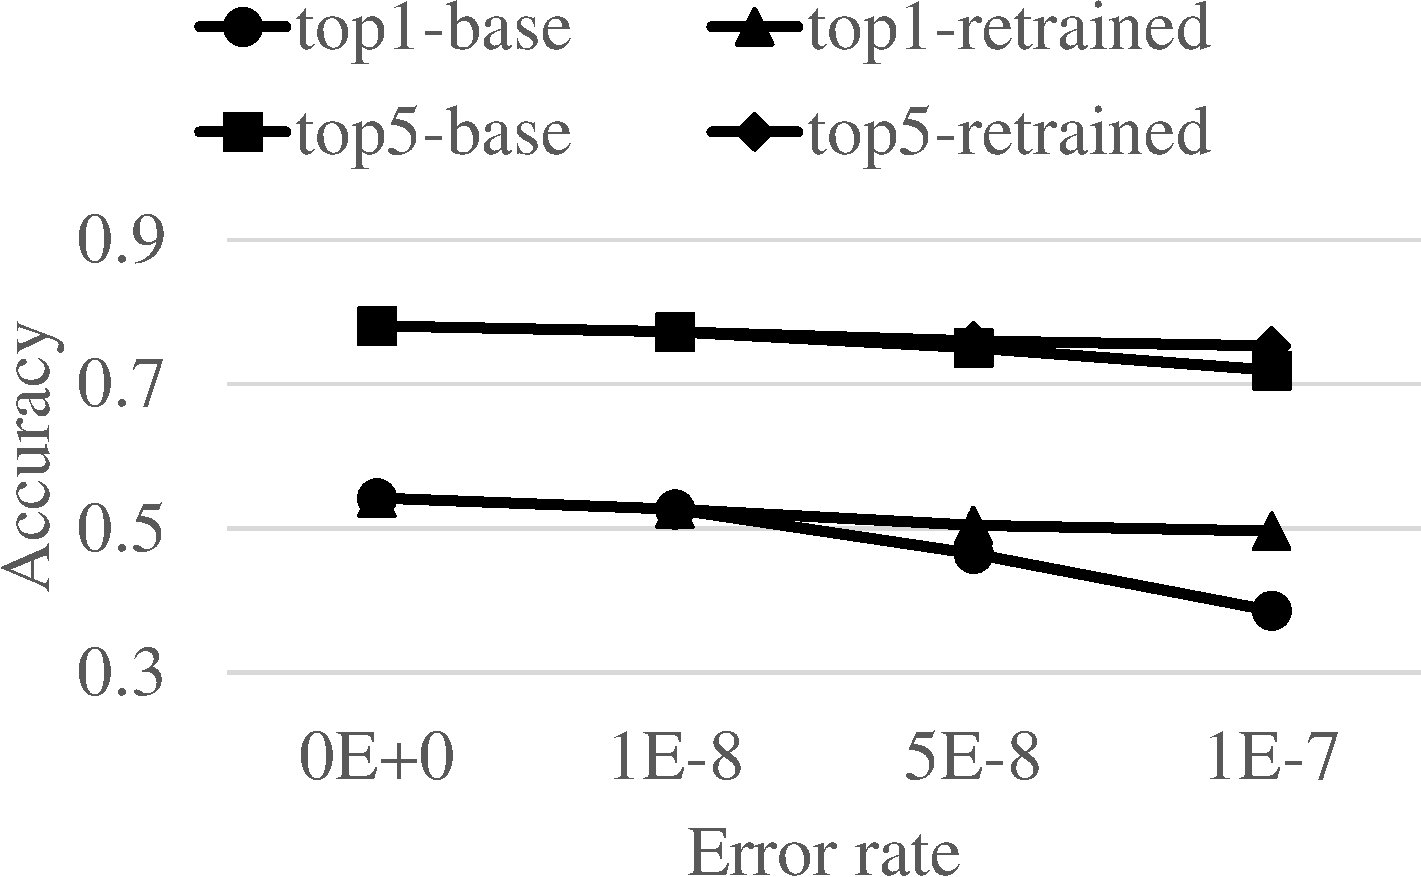
\includegraphics[width=0.7\linewidth]{alexnet-softerror}
        }
        \qquad
        \subfloat[VGG-16]{
                \label{fig:vgg16}
                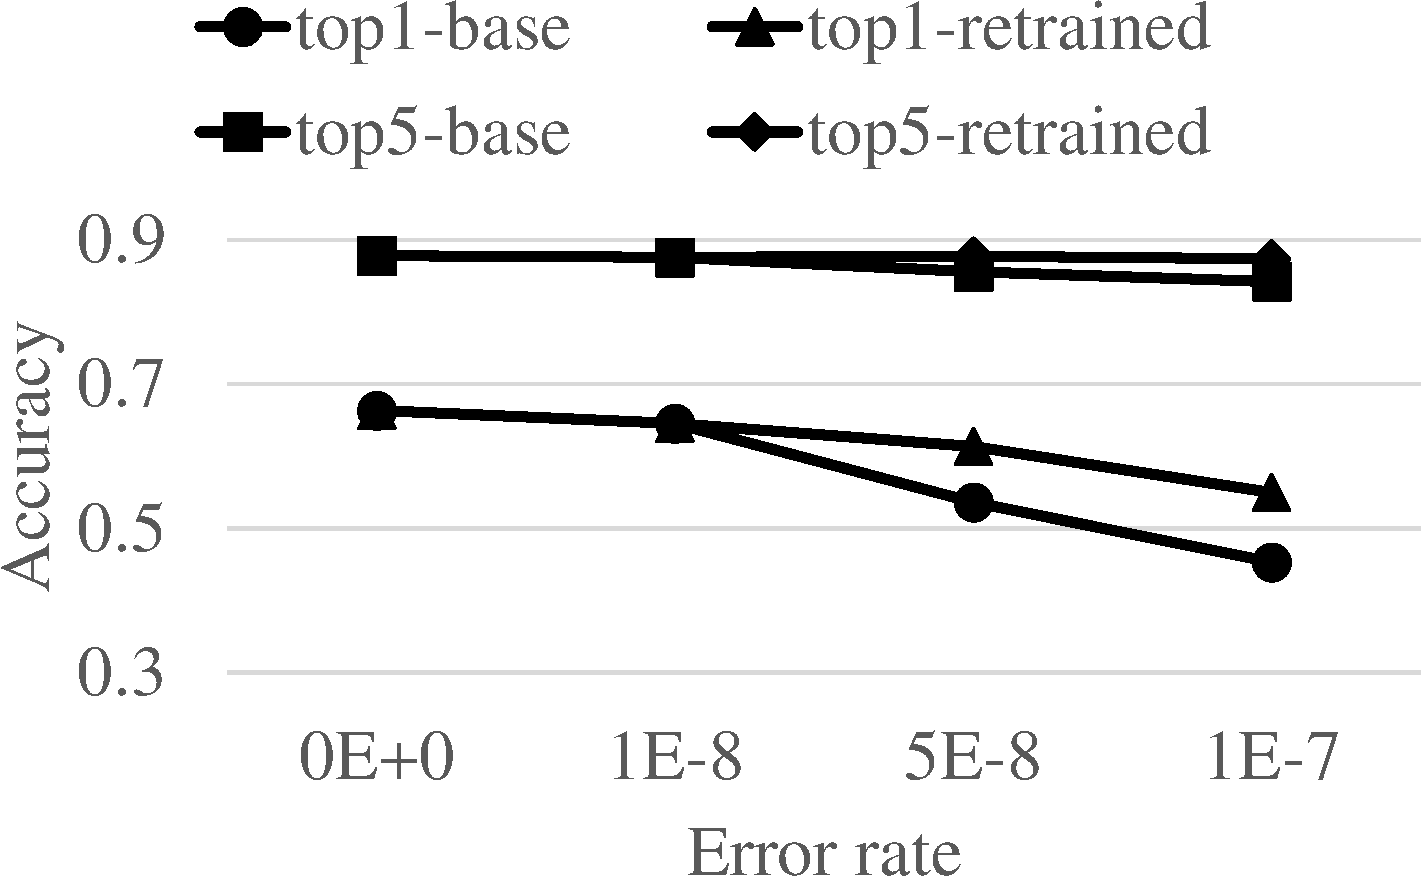
\includegraphics[width=0.7\linewidth]{vgg16-softerror}
        }
        \qquad
        \subfloat[VGG-19]{
                \label{fig:vgg19}
                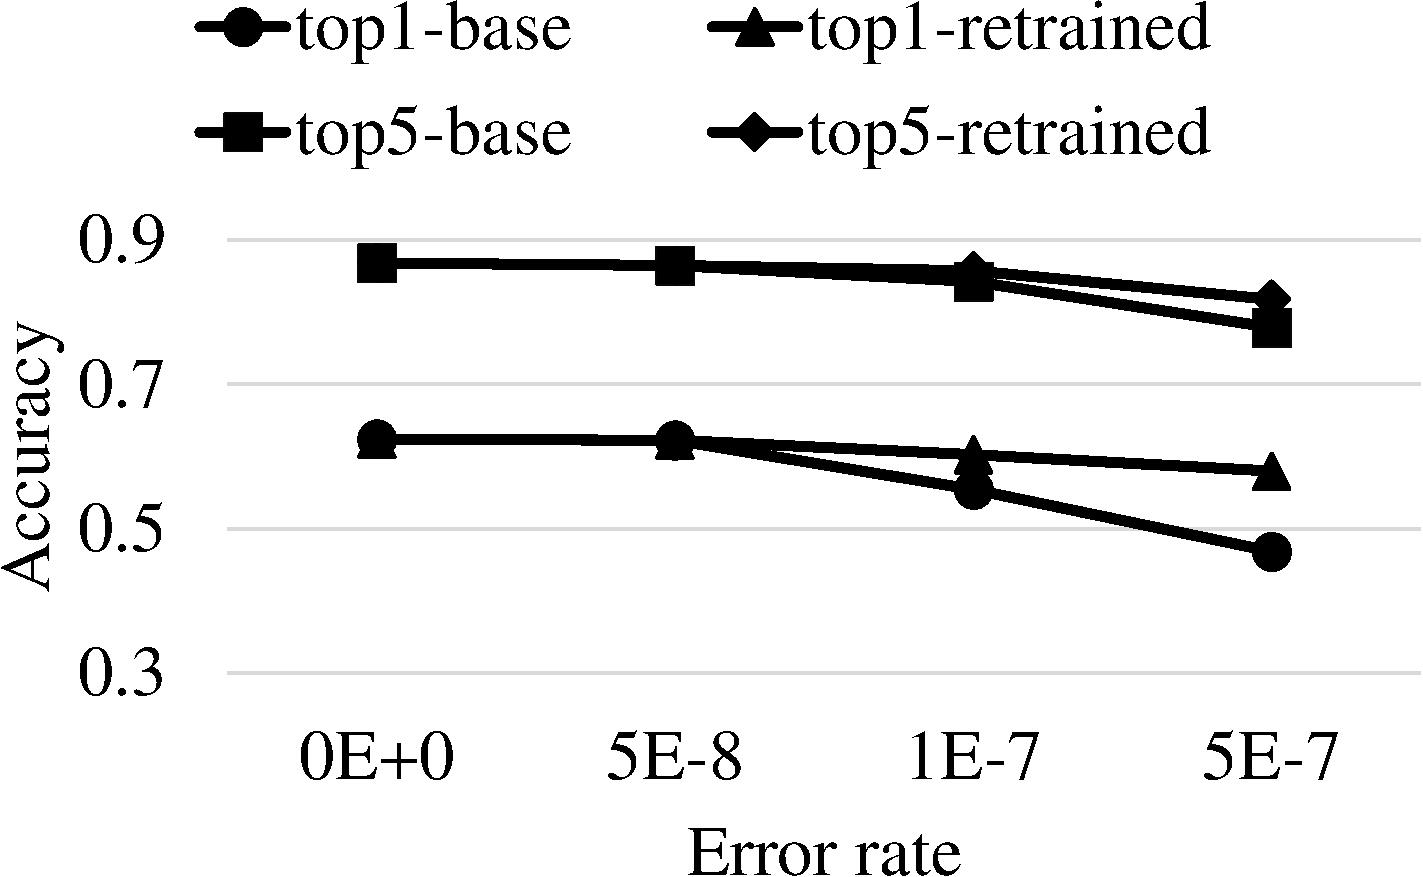
\includegraphics[width=0.7\linewidth]{vgg19-softerror}
        }
        \caption{The precision accuracy of the benchmark neural network models on accelerators with different computing errors}
        \label{fig:softerror-accuracy}
\end{figure}

\begin{figure}
        \center{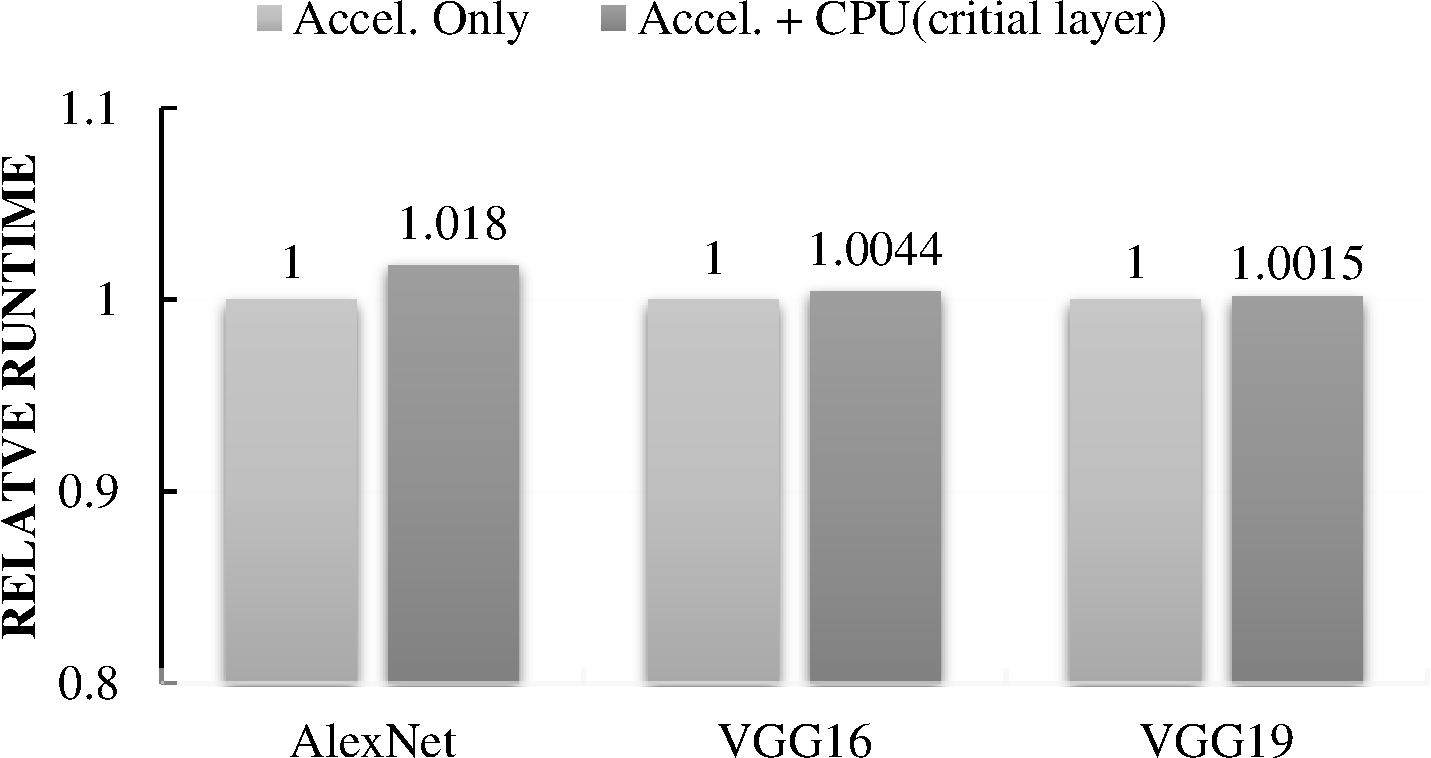
\includegraphics[width=0.7\linewidth]{clp_time}}
        \caption{Relative runtime of neural networks when the critical layer is scheduled to CPU.}
        \label{fig:clp_perf}
\end{figure}

We decide the critical layers using the error distribution as shown in Figure \ref{fig:clp_perf}.
We set the error threshold to be 5 and the experiment reveals that the last FC 
layer has the largest portion of computing errors that are more than 5. Thus, it is considered as 
the most critical layer. The critical layer takes only a small portion of the overall 
neural network computing, so the performance penalty is small even 
when it is scheduled to CPU. The last FC layer in AlexNet takes up higher portion of computing, 
the performance penalty is relatively higher compared to VGG16 and VGG19.
\begin{figure*}
        \center{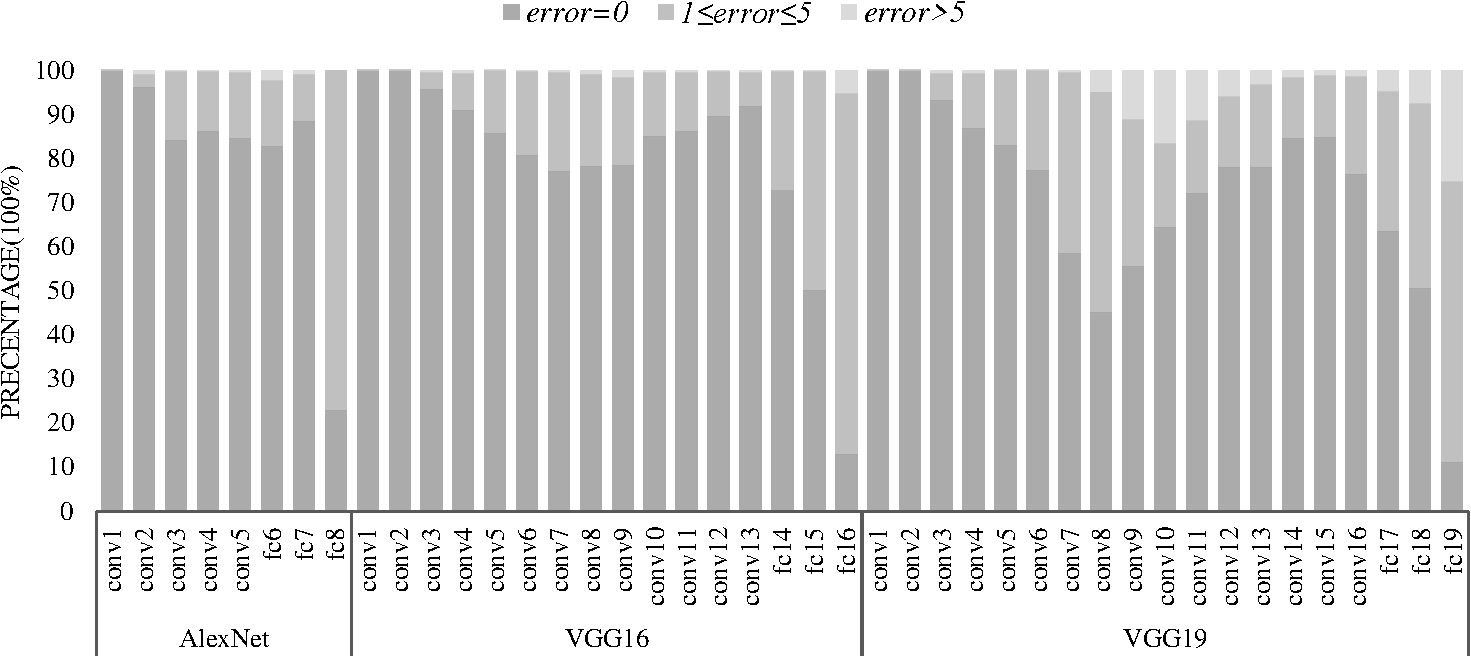
\includegraphics[width=0.8\linewidth]{error_distribute_softerror}}
        \caption{Error distribution across the neural network layers when highest BER is used in AlexNet, VGG16 and VGG19.}
        \label{fig:clp_perf}
\end{figure*}

\subsection{Overclocking case study}
To verify the proposed resilient training, we take overclocked CNN accelerator on KCU1500 as a case 
study in this work. By relaxing the timing constraints, the CNN accelerator can 
run at higher clock frequency with timing violations and computing errors. In PipeCNN, the 
hardware implementation is related to the neural network. For AlexNet, VGG16 and VGG19, the 
default implementation frequency is 210 MHz, 190 MHz and 190 MHz respectively. We then apply overclocking 
on the implementations with 10MHz step. The frequency can be boosted to 
260 MHz MHz, 240 MHz MHz and 240 MHz at most. By retraining the original neural network with 
the proposed approach, the prediction accuracy improvement is evaluated in detail.

With the overclocked CNN accelerators, we compare both the offline 
training and the proposed resilient training as presented in Figure \ref{fig:overclock-accuracy}. 
The prediction accuracy remains unchanged at the beginning and exhibits cliff-like drop 
at a tipping point. Beyond the tipping point, the prediction is no longer interesting 
due to the extremely low accuracy. At the tipping point, the top1 and top5 prediction accuracy of the 
retrained neural networks improves by xxx and xxx respectively.

\begin{figure}
        \center
	\subfloat[AlexNet]{
                \label{fig:alexnet}
                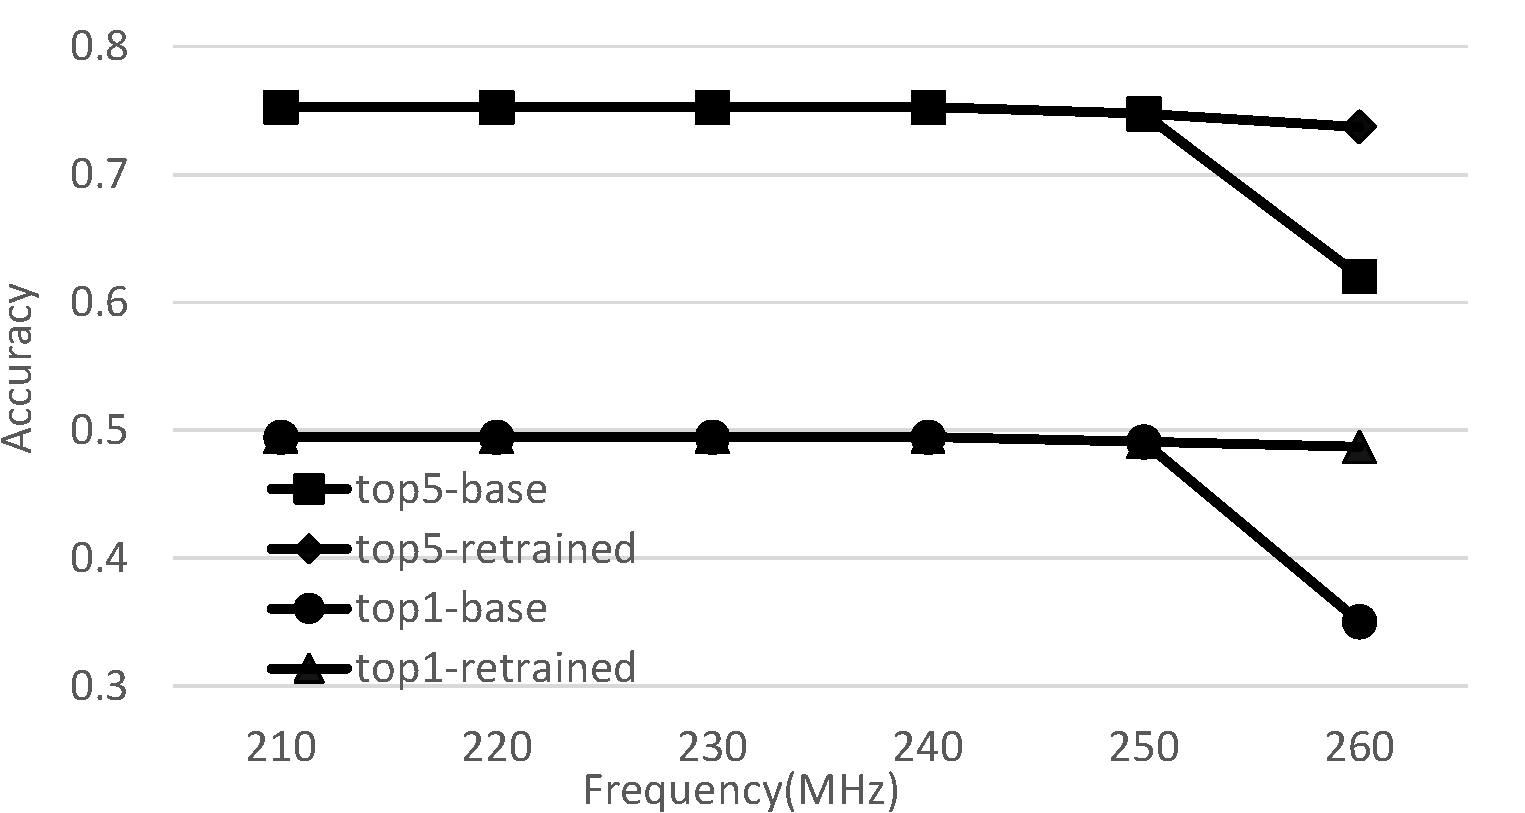
\includegraphics[width=0.6\linewidth]{alexnet-overclock}
        }
	\qquad
	\subfloat[VGG-16]{
                \label{fig:vgg16}
                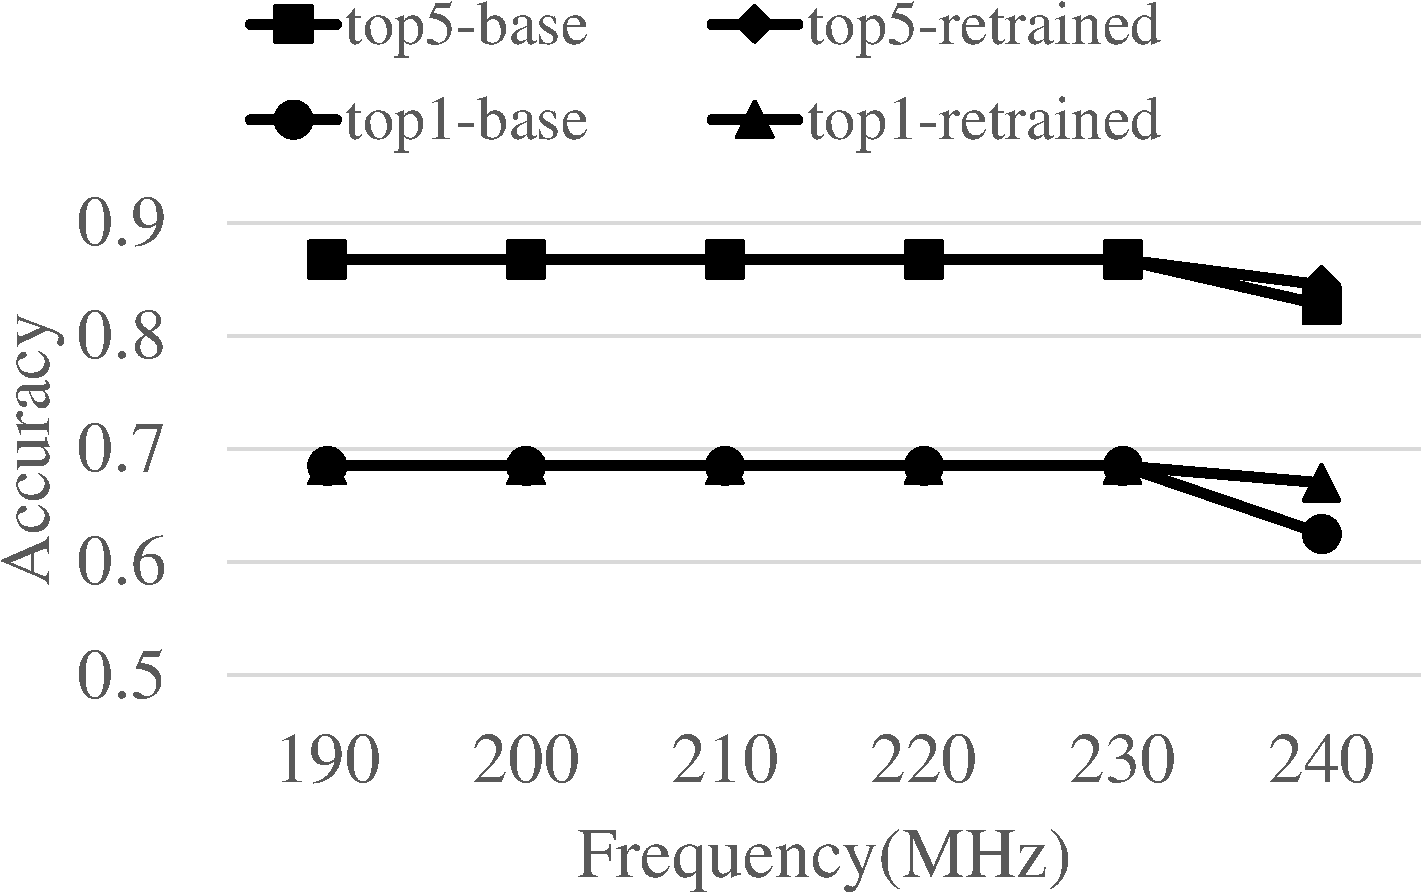
\includegraphics[width=0.6\linewidth]{vgg16-overclock}
        }
        \qquad
	\subfloat[VGG-19]{
                \label{fig:vgg19}
                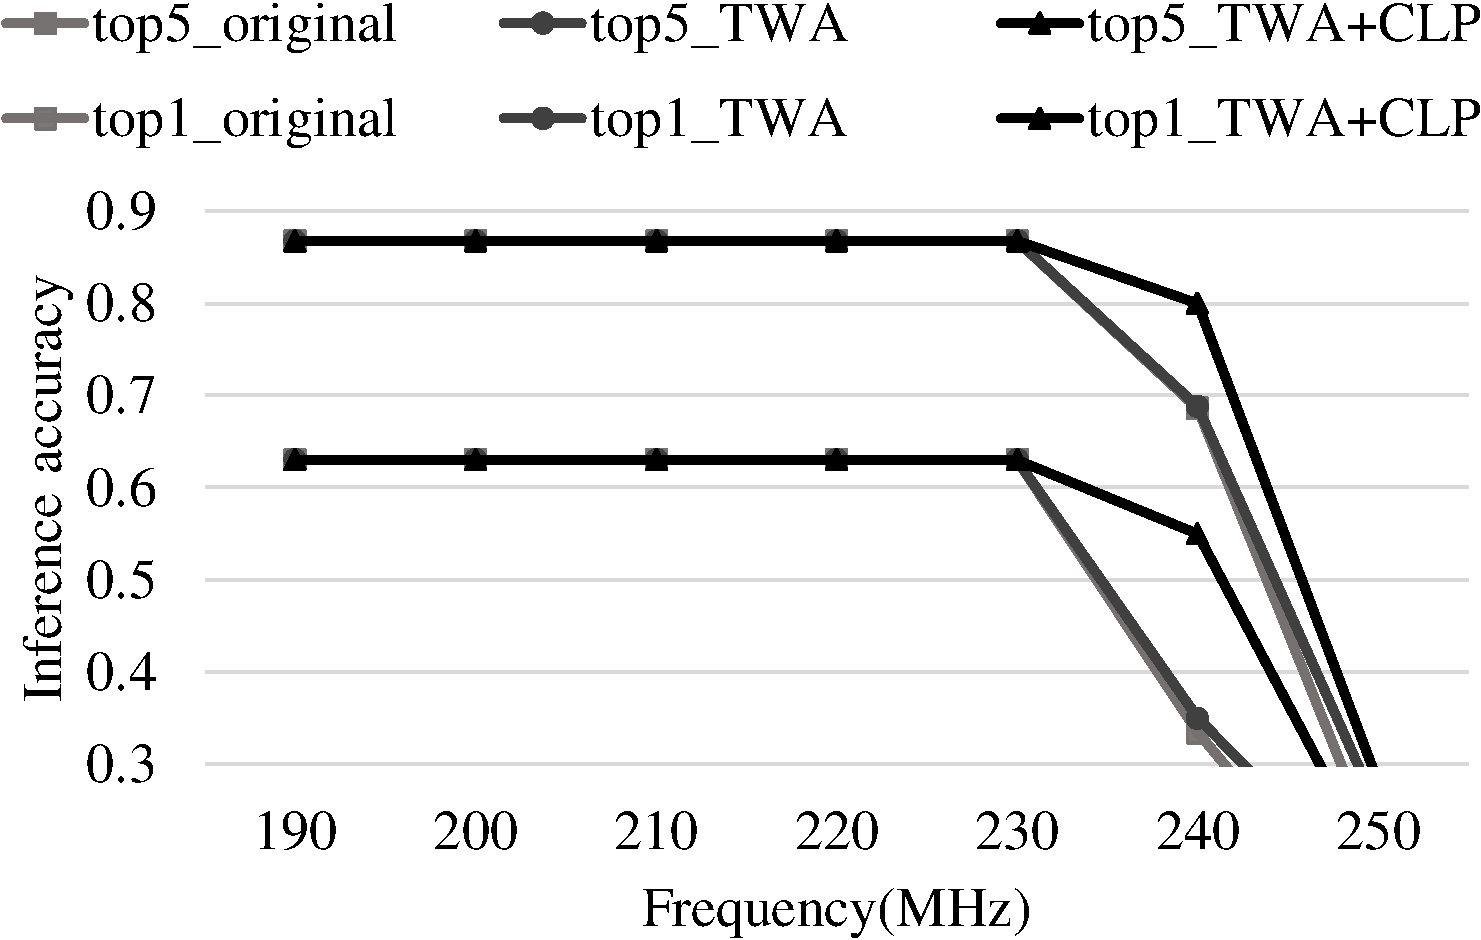
\includegraphics[width=0.6\linewidth]{vgg19-overclock}
        }
	\caption{The prediction accuracy of the benchmark neural networks on accelerators with different overclocking}
        \label{fig:overclock-accuracy}
\end{figure}

Clock frequency is almost proportional to the performance of the CNN accelerator 
especially for large convolution operation which is typically computing bound. 
Figure \ref{fig:overclocking-time} shows the relative inference runtime of the three neural networks at different 
overclocking. On the tipping point which is also the extreme overclocking case, 
the runtime improves by xxx compared to the models running on normal accelerator with 
xxx top1 accuracy loss and xxx top5 accuracy loss on average. 
\begin{figure}
        \center{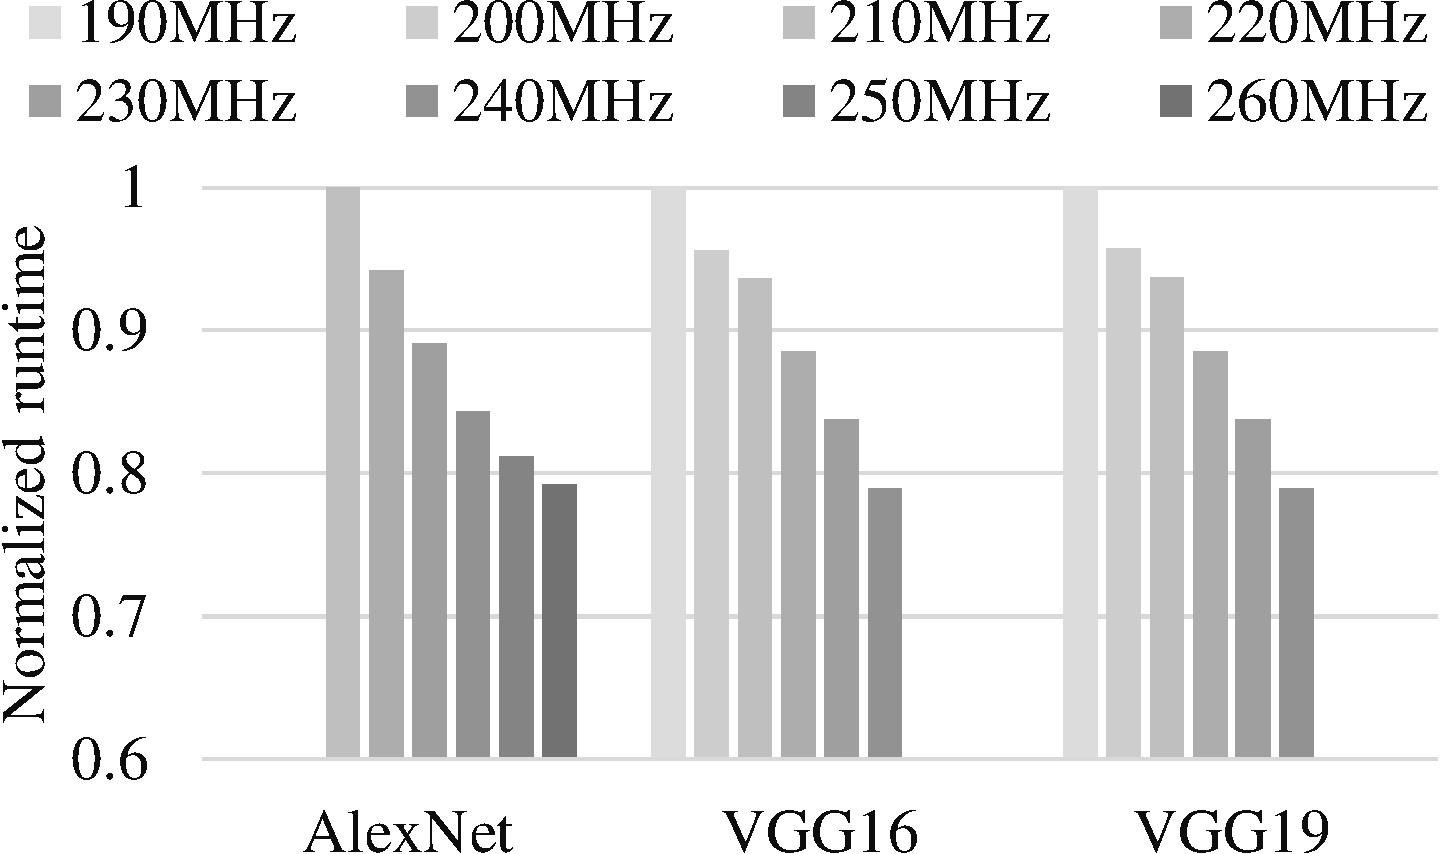
\includegraphics[width=0.6\linewidth]{relative-runtime}}
        \caption{Relative runtime of the neural networks on CNN accelerators with different overclocking. Note that AlexNet runs from 210 MHz to 250 MHz while 
		VGG16 and VGG19 ranges from 190 MHz to 240MHz, so some of the data is left blank.}
        \label{fig:overclocking-time}
\end{figure}

Comparing the experiments with random error simulation and overclocking on realistic FPGAs, we
find that the computing errors may not be uniformly distributed. In the overclocking,  
the prediction accuracy drops with cliff-like style. It indicates the computing errors may 
be quite small with light overclocking, but the amount of errors explodes at certain point.
Fortunately, the general trend is similar and the proposed training produces more resilient 
neural networks. 



% \section{Challenges \& Looking Forward}
% While the early results of using FPGA overlay are encouraging, there remain many challenges that must be overcome before its full potential can be unleashed.
%
%While the potential of FPGA overlay is plentiful, there remain many challenges lying ahead that warrant future research.
In particular, for FPGA overlays to be useful, future research must be able to address two important challenges: reduce overhead and enhance customization.

\subsubsection{Reducing Overhead}
By introducing an additional architectural layer between a user application and the physical fabric, an FPGA overlay inevitably incurs additional performance and area overhead to the system.
It is especially important when the FPGA is used as an accelerator in a processor-based system. 
If the overhead is so large that the FPGA is no longer offering any significant performance enhancement, then software programmers will have little incentive to devote effort into using them.

From a hardware implementation's point of view, the additional layer must also incur additional area overhead.
Such overhead usually manifests as additional usage of configurable fabric and on-chip memory.
In some cases where spare resources are available, the effect of such area overhead may not be apparent.
In fact, as illustrated earlier, researchers have deduced ways to make sure of such spare resources for debugging purposes \cite{Hung:2013:TSO:2435264.2435272}.
However, in other cases where the area of FPGA overlay results in a reduction of resources available to implement a user's design, then it is likely that this area overhead will translate into performance overhead.
On a circuit level, such area overhead may also manifest as additional delays impose on the critical path, resulting in overall performance loss.
Therefore in short, area overhead, if not well controlled, may easily translate into performance overhead.

Luckily, as mentioned in some early works, despite such overhead, the use of an overlay may still be worthwhile from a performance perspective.  For example in \cite{capalijia2013pipelined}, Capalija and Abdelrahman has demonstrated that by taking advantage of the regularity of its overlay and with the help of detailed floor planning, they were able to control the overhead while maintaining reasonable throughput performance when compared to a simple push-button synthesis flow.
The very use of overlay allows amortization of the optimization effort in the long run as the overlay structure may be reused many times.

\subsubsection{Enhancing Customization}
Another major challenge faced by overlay designers is the very notion of using FPGA overlay in the first place:
``If by overlaying a different architecture over an FPGA may provide all sort of nice properties, then why not implement the overlay architecture directly on silicon to enjoy all the benefits instead?''
For example, if a GPU overlay provides good performance and good programmability, then maybe the design should be implemented on an actual GPU instead of a GPU overlaying on top of an FPGA.

Indeed, if the so called ``overlay'' in question is simply a fixed reimplementation of another architecture on an FPGA, then the only incentive to so are probably to provide compatibility through virtualization, or simply to save cost on silicon implementation.
In the latter case, this intermediate architecture may hardly be called an ``overlay'' any more.

However, the true power of FPGA overlays is that they can be adapted to the application through \emph{customization}.
As a virtual architecture, many aspects of an overlay architecture can be customized to the target application to improve power-performance.
In \cite{Lebedev2010}, for example, the computational core in the multi-core overlay may be customized to the specific targeted application.
By customizing the core to their targeted application, almost 10x improvement in the overlay performance can be observed, bring the overlay performance to be within factor of 3 of the reference custom FPGA design.
In \cite{Lin:2012:EDC:2460216.2460227}, the direct connection topology among the process elements in coarse-grained reconfigurable array overlay was customized against the input application. 
When compared to the best predefined topology, the application-specific interconnect provides up to 28\% improvement in resulting energy-delay product.

The improved results should come at no surprise: the extreme case of an overlay customization is simply a full-custom design of the application on the target FPGA, which is supposed to have the best possible performance if designed correctly.
What is challenging is therefore to ability to fine-tune the tradeoff among design productivity, virtualization and performance of the resulting system.
In other word, the research question to ask in the future should therefore be: ``How to improve performance of an overlaying system through customization without significantly sacrificing the benefits of using an overlay?''
The answer to this question is going to open up a wide field of exciting research in FPGA-based reconfigurable systems.

\subsubsection{Closing Thoughts}
FPGA overlay is without doubt going to be an important part of future FPGA-based reconfigurable systems.
The potential is plentiful and we anticipate that overlaying technology will benefit all aspects of future reconfigurable systems, especially on the important aspect of design productivity.
With silicon technologies continue to evolve, the amount of available on-chip configurable resource is going to increase.
The abundance of high-performance configurable resources on FPGA will enable a new generation of systems that relies heavily on advanced overlay architectures for virtualization and to improve design productivity. 




%\section{State-of-the-art and availability/usability for software engineers}
%\input{current}

\bibliographystyle{alpha}
\bibliography{literature}

\end{document}
